%%% On-going present
%%
%% Beginning of file 'sample.tex'
%%
%% Modified 2005 December 5
%%
%% This is a sample manuscript marked up using the
%% AASTeX v5.x LaTeX 2e macros.

%% The first piece of markup in an AASTeX v5.x document
%% is the \documentclass command. LaTeX will ignore
%% any data that comes before this command.

%% The command below calls the preprint style  
%% which will produce a one-column, single-spaced document.
%% Examples of commands for other substyles follow. Use
%% whichever is most appropriate for your purposes.
%%
%%\documentclass[12pt,preprint]{aastex}

%% manuscript produces a one-column, double-spaced document:

%%\documentclass[manuscript]{aastex}

%% preprint2 produces a double-column, single-spaced document:

 %\documentclass[preprint2]{aastex}
%\documentclass[preprint2]{aastex}
%\documentclass[manuscript]{aastex}
\documentclass[iop]{emulateapj}
\renewcommand{\baselinestretch}{0.95}
%% Sometimes a paper's abstract is too long to fit on the
%% title page in preprint2 mode. When that is the case,
%% use the longabstract style option.

%% \documentclass[preprint2,longabstract]{aastex}

%% If you want to create your own macros, you can do so
%% using \newcommand. Your macros should appear before
%% the \begin{document} command.
%%
%% If you are submitting to a journal that translates manuscripts
%% into SGML, you need to follow certain guidelines when preparing
%% your macros. See the AASTeX v5.x Author Guide
%% for information.

\usepackage{enumitem} 

\newcommand{\hMsun}{{\ifmmode{h^{-1}{\rm
        {M_{\odot}}}}\else{$h^{-1}{\rm{M_{\odot}}}$~}\fi}} 
\newcommand{\hMpc}{{\ifmmode{h^{-1}{\rm Mpc}}\else{$h^{-1}$Mpc }\fi}}
\def\be{\begin{equation}}
\def\ee{\end{equation}}
\def\ba{\begin{eqnarray}}
\def\ea{\end{eqnarray}}


%% You can insert a short comment on the title page using the command below.

%\slugcomment{Not to appear in Nonlearned J., 45.}

%% If you wish, you may supply running head information, although
%% this information may be modified by the editorial offices.
%% The left head contains a list of authors,
%% usually a maximum of three (otherwise use et al.).  The right
%% head is a modified title of up to roughly 44 characters.
%% Running heads will not print in the manuscript style.

%\title[]
%{}

\shorttitle{Significantly improved dark energy figure of merit from reshift dependence of AP effect}
\shortauthors{X.-D. Li, C.G. Sabiu, C. Park, Y. Wang, G.-B. Zhao, H. Park, A. Shafieloo, J. Kim, S.E. Hong}

%% This is the end of the preamble.  Indicate the beginning of the
%% paper itself with \begin{document}.

\begin{document}

%% LaTeX will automatically break titles if they run longer than
%% one line. However, you may use \\ to force a line break if
%% you desire.

\title{Cosmological constraints from the redshift dependence of the Alcock-Paczynski effect: 
significant improvement in the dark energy figure of merit}


%\author{Xiao-Dong~Li\altaffilmark{1}, Changbom~Park\altaffilmark{1}, J.~E.~Forero-Romero\altaffilmark{2} and Juhan Kim%\altaffilmark{3}}
%\affil{\altaffilmark{1}School of Physics, Korea Institute for Advanced Study, Heogiro 85, Seoul 130-722, Korea }
%\affil{\altaffilmark{2}Departamento de F\'{i}sica, Universidad de los Andes, Cra. 1 No. 18A-10, Edificio Ip, Bogot\'a, %Colombia}
%\affil{\altaffilmark{3}Center for Advanced Computation, Korea Institute for Advanced Study, 85 Hoegi-ro, Dongdaemun-%gu, Seoul 130-722, Korea }
%\affil{\it (xiaodongli@kias.re.kr, cbp@kias.re.kr, je.forero@uniandes.edu.co, kjhan@kias.re.kr)}

%\author[Xiao-Dong~Li, Changbom~Park, Cristiano G. Sabiu, Juhan Kim and Sungwook E. Hong]
%{ Xiao-Dong Li$^{1,\dagger}$, Changbom Park$^{1}$, Cristiano G. Sabiu$^{2}$, Juhan Kim$^{3,1,\star}$, Sungwook E. Hong$^{1}$\\
%$^1$School of Physics, Korea Institute for Advanced Study, 85 Heogi-ro, Dongdaemun-gu, Seoul 130-722, Korea\\
%$^2$Korea Astronomy and Space Science Institute, 776, Daedeokdae-ro, Yuseong-gu, Daejeon, 305-348, Korea\\
%$^3$Center for Advanced Computation, Korea Institute for Advanced Study, 85 Hoegi-ro, Dongdaemun-gu, Seoul 130-722, Korea\\
%$^{\dagger}$xiaodongli@kias.re.kr\\
%$\star$Corresponding Author: ***@kasi.re.kr}

%[Xiao-Dong~Li, Cristiano G. Sabiu, Yuting Wang, Changbom~Park, Gong-bo Zhao, Hyunbae Park, Arman Shafieloo, Juhan Kim and Sungwook E. Hong]
\author{Xiao-Dong~Li$^{1,2}$, Cristiano G. Sabiu$^3$, Yuting Wang$^4$, Changbom~Park$^2$, Gong-bo Zhao$^4$, Hyunbae Park$^3$, Arman Shafieloo$^3$, Juhan Kim$^5$ and Sungwook E. Hong$^3$}
%{ Xiao-Dong Li$^{1,2,\dagger}$, Changbom Park$^{1}$, Cristiano G. Sabiu$^{2}$, Juhan Kim$^{3,1,\star}$, Sungwook E. Hong$^{1}$\\
\affil{$^1$School of Physics and Astronomy, Sun Yat-Sen University, Guangzhou 510297, P.R.China}
\affil{$^2$School of Physics, Korea Institute for Advanced Study, 85 Heogiro, Dongdaemun-gu, Seoul 02455, Korea}
\affil{$^3$Korea Astronomy and Space Science Institute, 776, Daedeokdae-ro, Yuseong-gu, Daejeon, 34055, Korea}
\affil{$^4$National Astronomy Observatories, Chinese Academy of Science, Beijing, 100012, P.R.China}
\affil{$^5$Center for Advanced Computation, Korea Institute for Advanced Study, 85 Hoegi-ro, Dongdaemun-gu, Seoul 02455, Korea}

%\author{Xiao-Dong Li,}
%\affil{School of Physics and Astronomy, SYSU TBA}
%\affil{School of Physics, Korea Institute for Advanced Study, 85 Heogiro, Dongdaemun-gu, Seoul 02455, Korea}
%\author{Cristiano G. Sabiu,}
%\affil{Korea Astronomy and Space Science Institute, 776, Daedeokdae-ro, Yuseong-gu, Daejeon, 34055, Korea}
%\author{Changbom Park,}
%\affil{School of Physics, Korea Institute for Advanced Study, 85 Heogiro, Dongdaemun-gu, Seoul 02455, Korea}
%\author{Yuting Wang, Gong-bo Zhao}
%\affil{National Astronomy Observatories, Chinese Academy of Science, Beijing, 100012, P.R.China}
%\author{Hyunbae Park, Arman Shafieloo,}
%\affil{Korea Astronomy and Space Science Institute, 776, Daedeokdae-ro, Yuseong-gu, Daejeon, 34055, Korea}
%\author{Juhan Kim,}
%\affil{Center for Advanced Computation, Korea Institute for Advanced Study, 85 Hoegi-ro, Dongdaemun-gu, Seoul 02455, Korea}
%\author{and Sungwook E. Hong}
%\affil{Korea Astronomy and Space Science Institute, 776, Daedeokdae-ro, Yuseong-gu, Daejeon, 34055, Korea}

%\altaffiltext{1}{xiaodongli@kias.re.kr}
%\altaffiltext{2}{cbp@kias.re.kr}
%\altaffiltext{3}{csabiu@kasi.re.kr}
%\altaffiltext{4}{\bf Hyunbae: your email}
%\altaffiltext{1}{Corresponding Author: kjhan@kias.re.kr}

% \email{xiaodongli@kias.re.kr}
% \email{cbp@kias.re.kr}
% \email{je.forero@uniandes.edu.co}



% \author{S. Djorgovski\altaffilmark{1,2,3} and Ivan R. King\altaffilmark{1}}
% \affil{Astronomy Department, University of California,
%     Berkeley, CA 94720}
%
% \author{C. D. Biemesderfer\altaffilmark{4,5}}
% \affil{National Optical Astronomy Observatories, Tucson, AZ 85719}
% \email{aastex-help@aas.org}
%
% \and
%
% \author{R. J. Hanisch\altaffilmark{5}}
% \affil{Space Telescope Science Institute, Baltimore, MD 21218}
%
% %% Notice that each of these authors has alternate affiliations, which
% %% are identified by the \altaffilmark after each name.  Specify alternate
% %% affiliation information with \altaffiltext, with one command per each
% %% affiliation.
%
% \altaffiltext{1}{Visiting Astronomer, Cerro Tololo Inter-American Observatory.
% CTIO is operated by AURA, Inc.\ under contract to the National Science
% Foundation.}
% \altaffiltext{2}{Society of Fellows, Harvard University.}
% \altaffiltext{3}{present address: Center for Astrophysics,
%     60 Garden Street, Cambridge, MA 02138}
% \altaffiltext{4}{Visiting Programmer, Space Telescope Science Institute}
% \altaffiltext{5}{Patron, Alonso's Bar and Grill}

%% Mark off your abstract in the ``abstract'' environment. In the manuscript
%% style, abstract will output a Received/Accepted line after the
%% title and affiliation information. No date will appear since the author
%% does not have this information. The dates will be filled in by the
%% editorial office after submission.

\begin{abstract}
We derive tight constraints on dynamical dark energy 
from the Alcock-Paczynski (AP) test via the redshift dependence of clustering on scales of 6 -- 40 $h^{-1}\rm Mpc$
to place constraints on the expansion history of the Universe.
We use the 1,133,326 galaxies from the Sloan Digital Sky Survey Data Release 12, 
spanning the redshift range $0.15<z<0.69$.
%Concentrating on the Chevallier-Polarski-Linder parametrization of dark energy, $w=w_0+w_a\frac{z}{1+z}$,
%while improving upon earlier works \citep{Li2016},
%we present a novel use of the Alcock-Paczynski (AP) test via clustering difference between redshift bins on scales of 6-40 $h^{-1}\rm Mpc$.
%This differential measure is shown to be a robust statistical tool that mitigates many systematic effects, 
%allowing for competitive and unbiased constrains to be placed on cosmological parameters.
We improve the methodology of Li et al. to enable efficient exploring of three or more cosmological parameters,
and apply it to the Chevallier-Polarski-Linder parametrization of dark energy, $w=w_0+w_a{z}/({1+z})$.
In combination with the CMB, BAO, SNIa and $H_0$ from Cepheid data, we obtain
$\Omega_m = 0.301 \pm 0.008,\ w_0 = -1.042 \pm 0.067,\ $ and $w_a = -0.07 \pm 0.29$ (68.3\% CL). 
Adding our new AP measurements to the aforementioned results 
reduces the error bars by $\sim$30 -- 40\%
%and reduces the area of $w_0-w_a$ contour by 50\%.
and improves the dark energy figure of merit by a factor of 2. 
We check the robustness of the results.
%The AP method may %be combined with the standard BAO method,
%greatly increase the power of ongoing and future galaxy surveys in probing dark energy.
\end{abstract}

%% Keywords should appear after the \end{abstract} command. The uncommented
%% example has been keyed in ApJ style. See the instructions to authors
%% for the journal to which you are submitting your paper to determine
%% what keyword punctuation is appropriate.

\keywords{large-scale structure of Universe --- dark energy --- cosmological parameters}

%% From the front matter, we move on to the body of the paper.
%% In the first two sections, notice the use of the natbib \citep
%% and \citet commands to identify citations.  The citations are
%% tied to the reference list via symbolic KEYs. The KEY corresponds
%% to the KEY in the \bibitem in the reference list below. We have
%% chosen the first three characters of the first author's name plus
%% the last two numeral of the year of publication as our KEY for
%% each reference.


%% Authors who wish to have the most important objects in their paper
%% linked in the electronic edition to a data center may do so by tagging
%% their objects with \objectname{} or \object{}.  Each macro takes the
%% object name as its required argument. The optional, square-bracket
%% argument should be used in cases where the data center identification
%% differs from what is to be printed in the paper.  The text appearing
%% in curly braces is what will appear in print in the published paper.
%% If the object name is recognized by the data centers, it will be linked
%% in the electronic edition to the object data available at the data centers
%%
%% Note that for sources with brackets in their names, e.g. [WEG2004] 14h-090,
%% the brackets must be escaped with backslashes when used in the first
%% square-bracket argument, for instance, \object[\[WEG2004\] 14h-090]{90}).
%%  Otherwise, LaTeX will issue an error.

\section{Introduction}

\begin{figure*}
   \centering{
   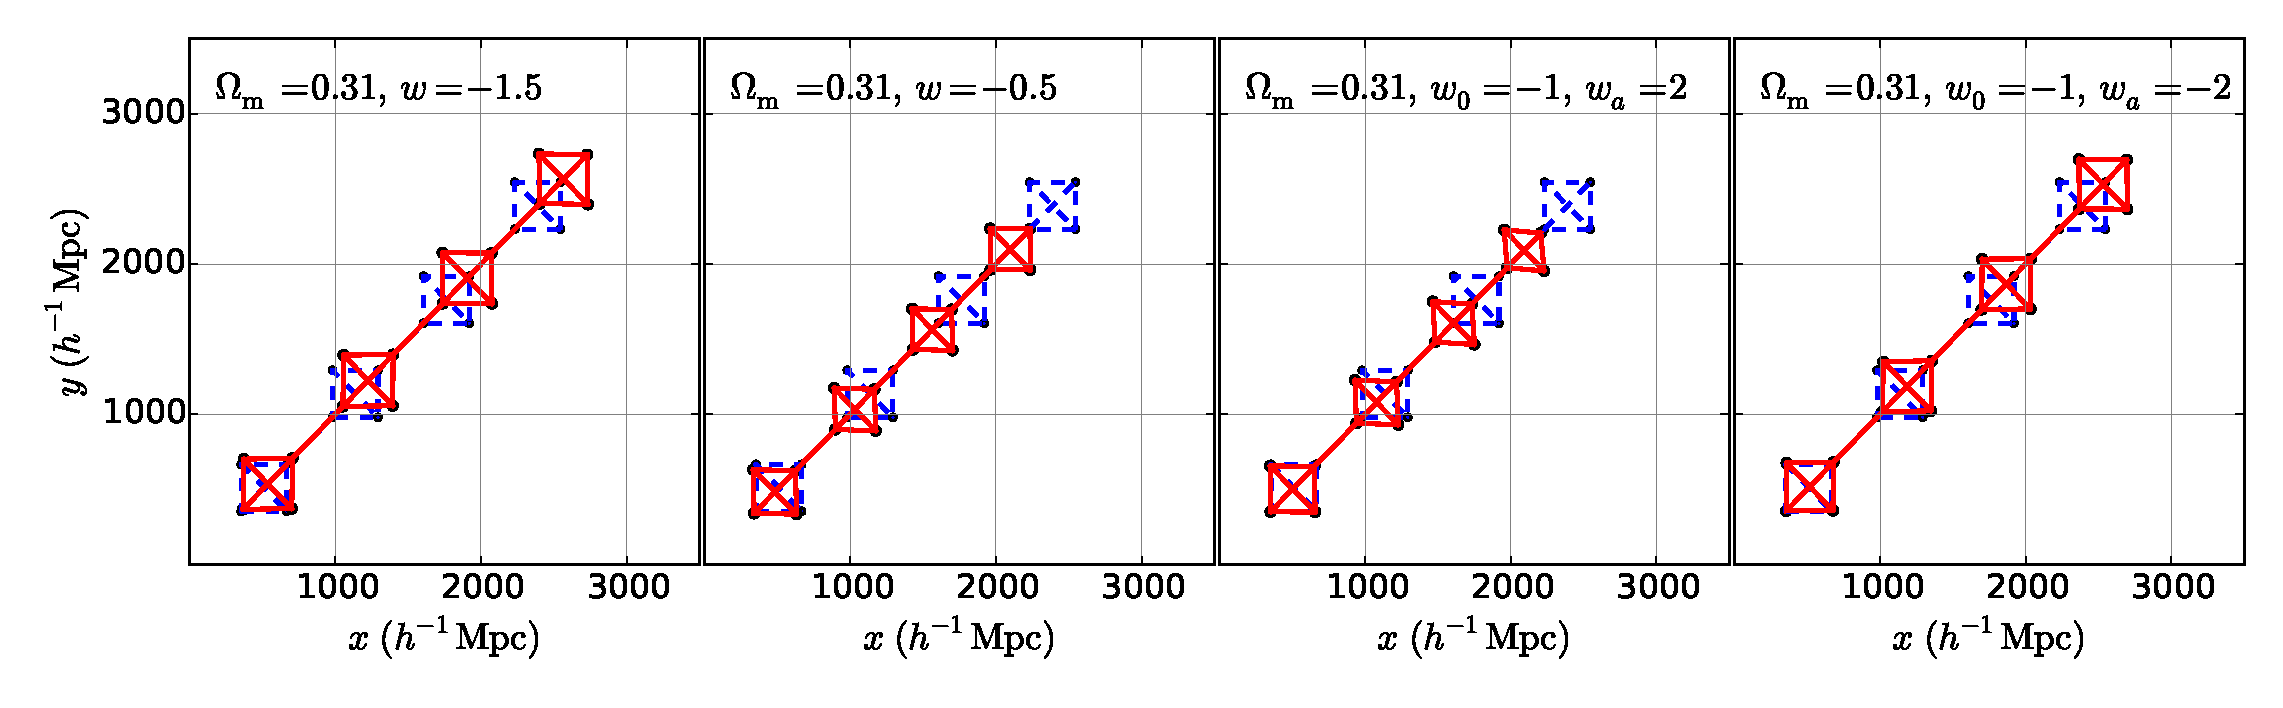
\includegraphics[height=5cm]{fig_xy.eps}
   %\includegraphics[height=8cm]{fig4_1.eps}
   %\includegraphics[height=7cm]{FVol.eps}
   %\includegraphics[height=8cm]{xy.eps}
   %\includegraphics[height=8cm]{smu.eps}
   }
   \caption{\label{fig_xy}
   %The distance dependence of the shape distortion in four wrongly assumed cosmologies,
   %assuming a true cosmology of $\Omega_m=0.26$, $w=-1$.
   %There are four perfect squares with their true shapes plotted in blue dashed lines.
   %They are measured by an observer located at the origin, and the distances are reprojected in the four wrong cosmologies.
   %The apparently distorted shapes are plotted in red solid lines.
   Examples of the rectangular shape distorted by assuming incorrect 
   cosmologies compared to the true fiducial cosmology $\Omega_m=0.26$ and $w=-1$.
   The blue dashed boxes mark the reference rectangular shape
   and the red distorted boxes are the shapes observed at the coordinate origin.
   }
\end{figure*}


%\begin{figure*}
%   \centering{
%   %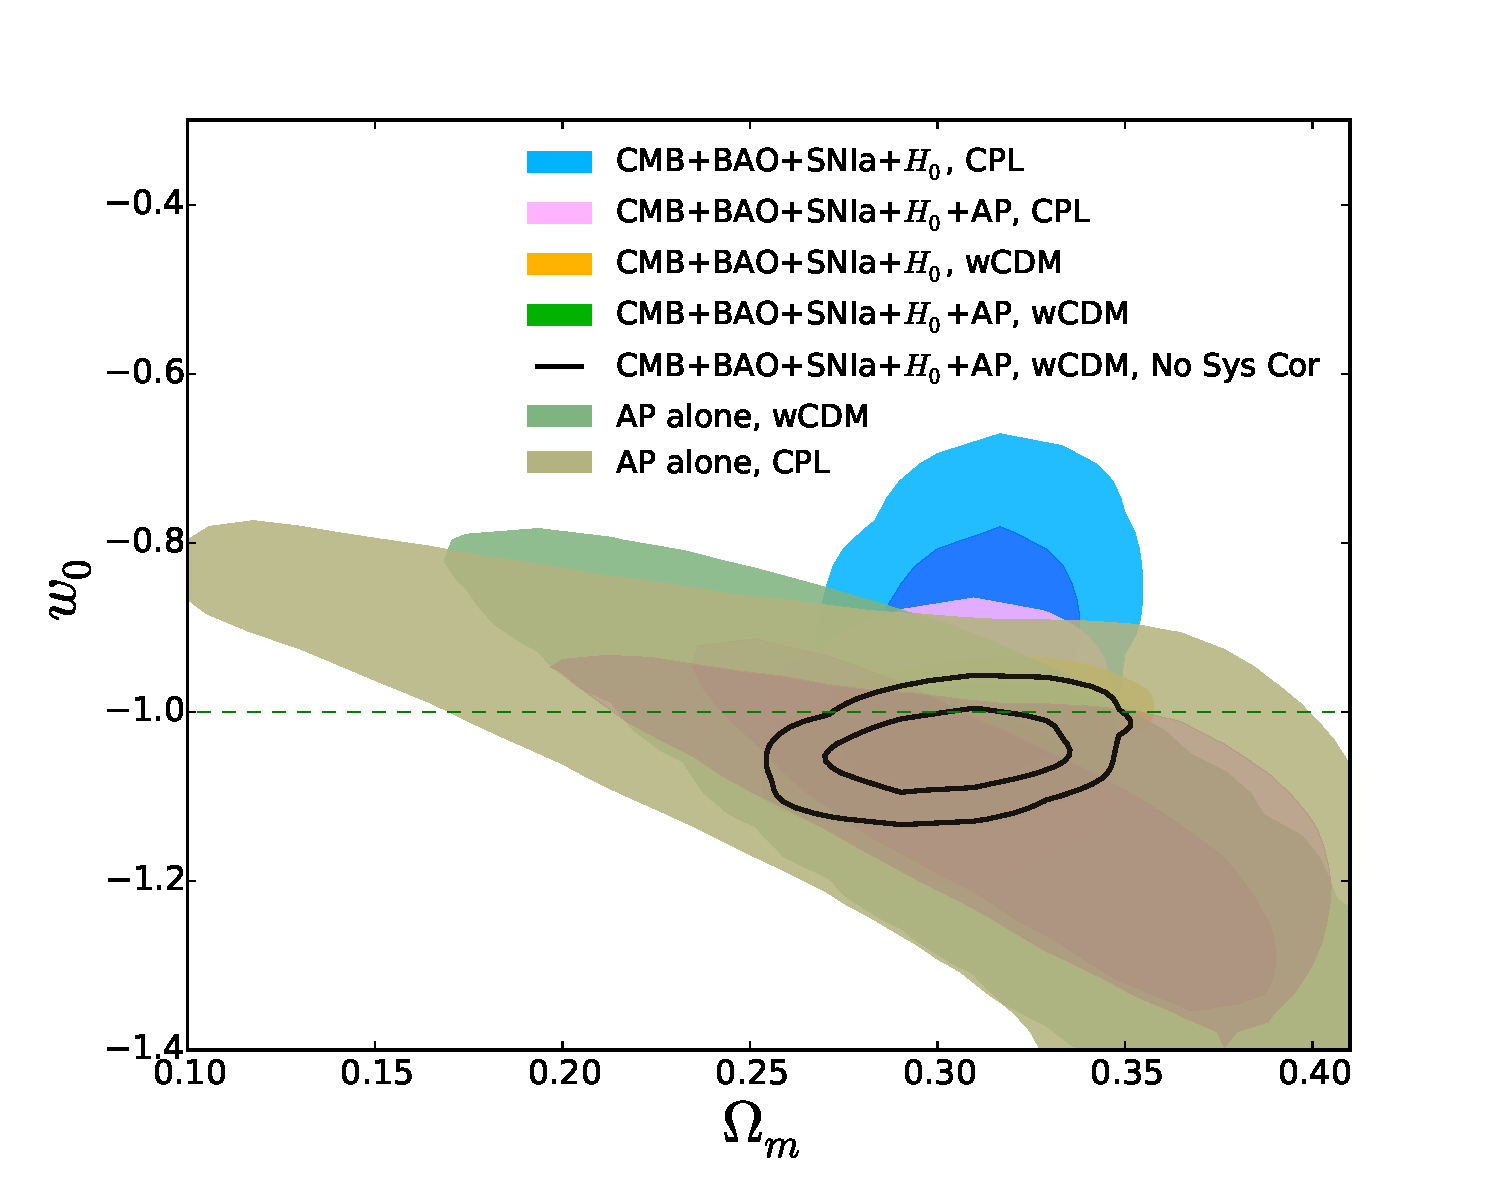
\includegraphics[width=9cm,natwidth=4,natheight=4]{figCPL_a.pdf}
%   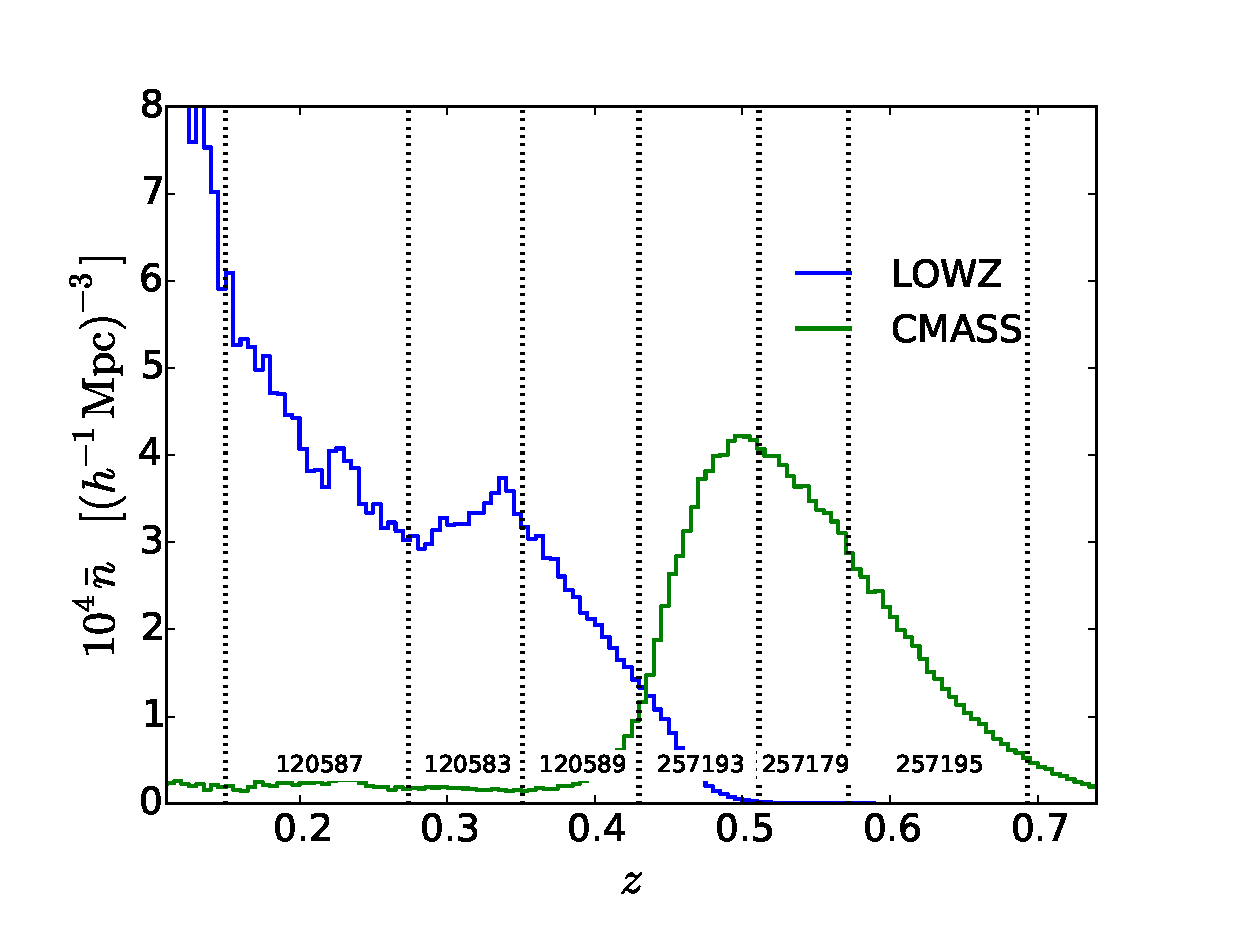
\includegraphics[height=6.5cm]{fig_nbar.eps}
%   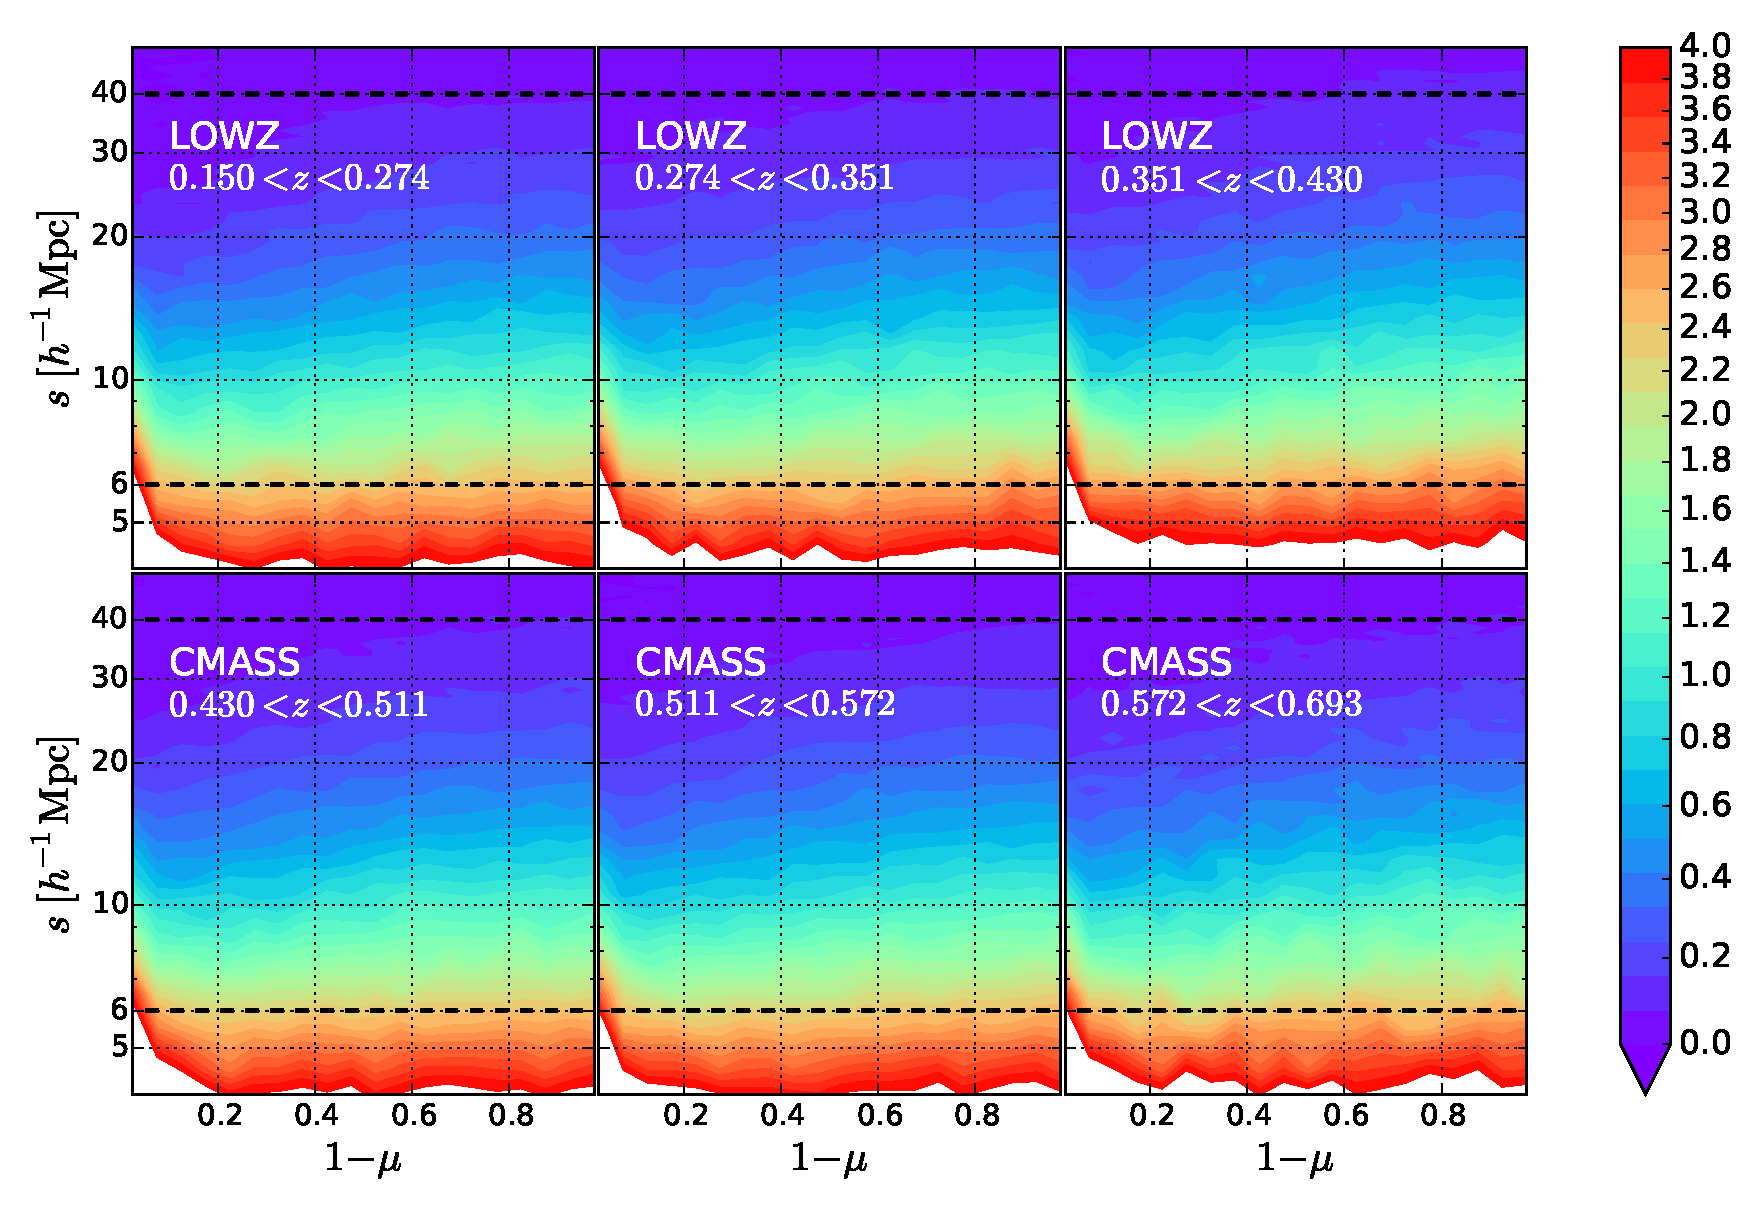
\includegraphics[width=9.0cm,]{fig_2pcf.eps}
%   }
%   \caption{\label{fig_TpCF}
%   Splitting the SDSS galaxies into six redshift bins, and measuring the correlation function
%   (similar figures already presented in \cite{Li2016}).
%   Left panel: We split the BOSS DR12 galaxies into six redshift bins to measure the evolution of shape distortion.
%   The blue and green solid histograms show the redshift density distribution of LOWZ and CMASS galaxies in the $\Omega_m=0.31$ $\Lambda$CDM. 
%   The vertical dashed lines define the six redshift bins that are used to cut the samples.
%   The number of LOWZ/CMASS galaxies in the three low/high redshift bins are listed.
%   Right panel: 2D contour map of measured $\xi$ as a function of $\mu$ and $s$, from the six redshift bins of LOWZ and CMASS samples, 
%      in the cosmology of $\Omega_m=0.31$ $\Lambda$CDM model.
%    The black dashed lines mark the clustering region 6-40\ Mpc/h studied in the AP method.
%    The six contour maps have rather similar appearance, implying small redshift evolution of $\xi$ from RSD.
%   }
%\end{figure*}

\begin{figure*}
   \centering{
   %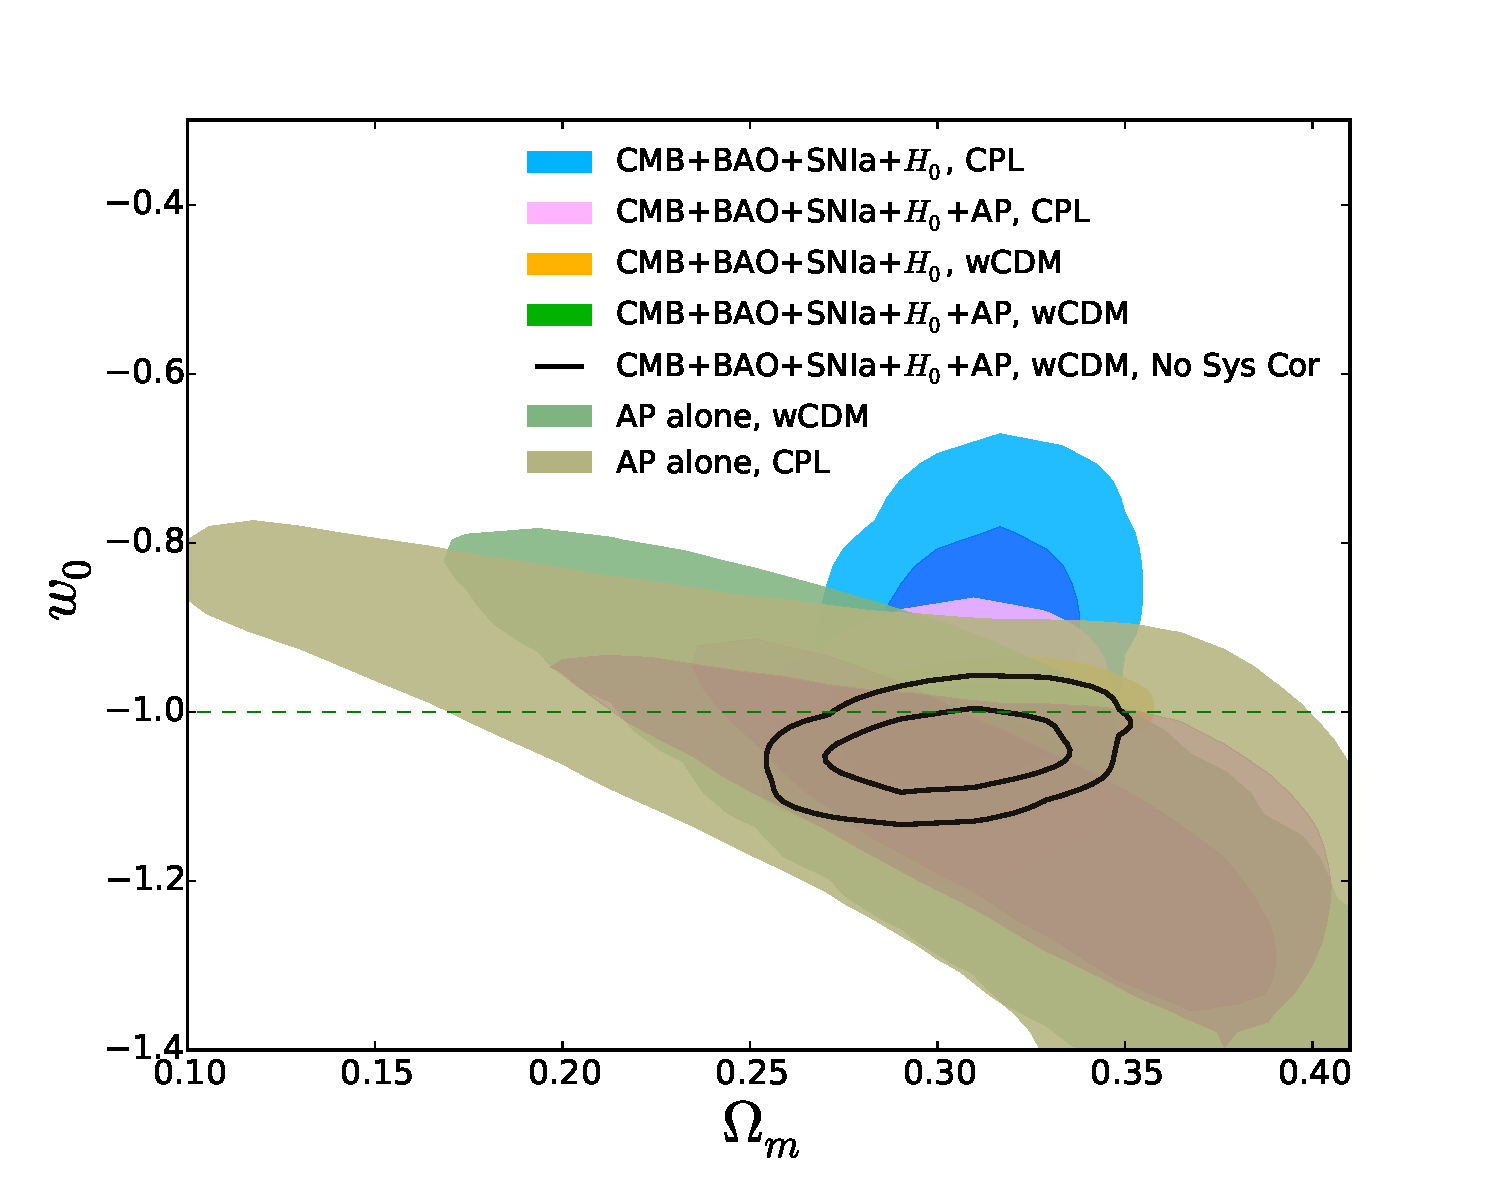
\includegraphics[width=9cm,natwidth=4,natheight=4]{figCPL_a.pdf}
   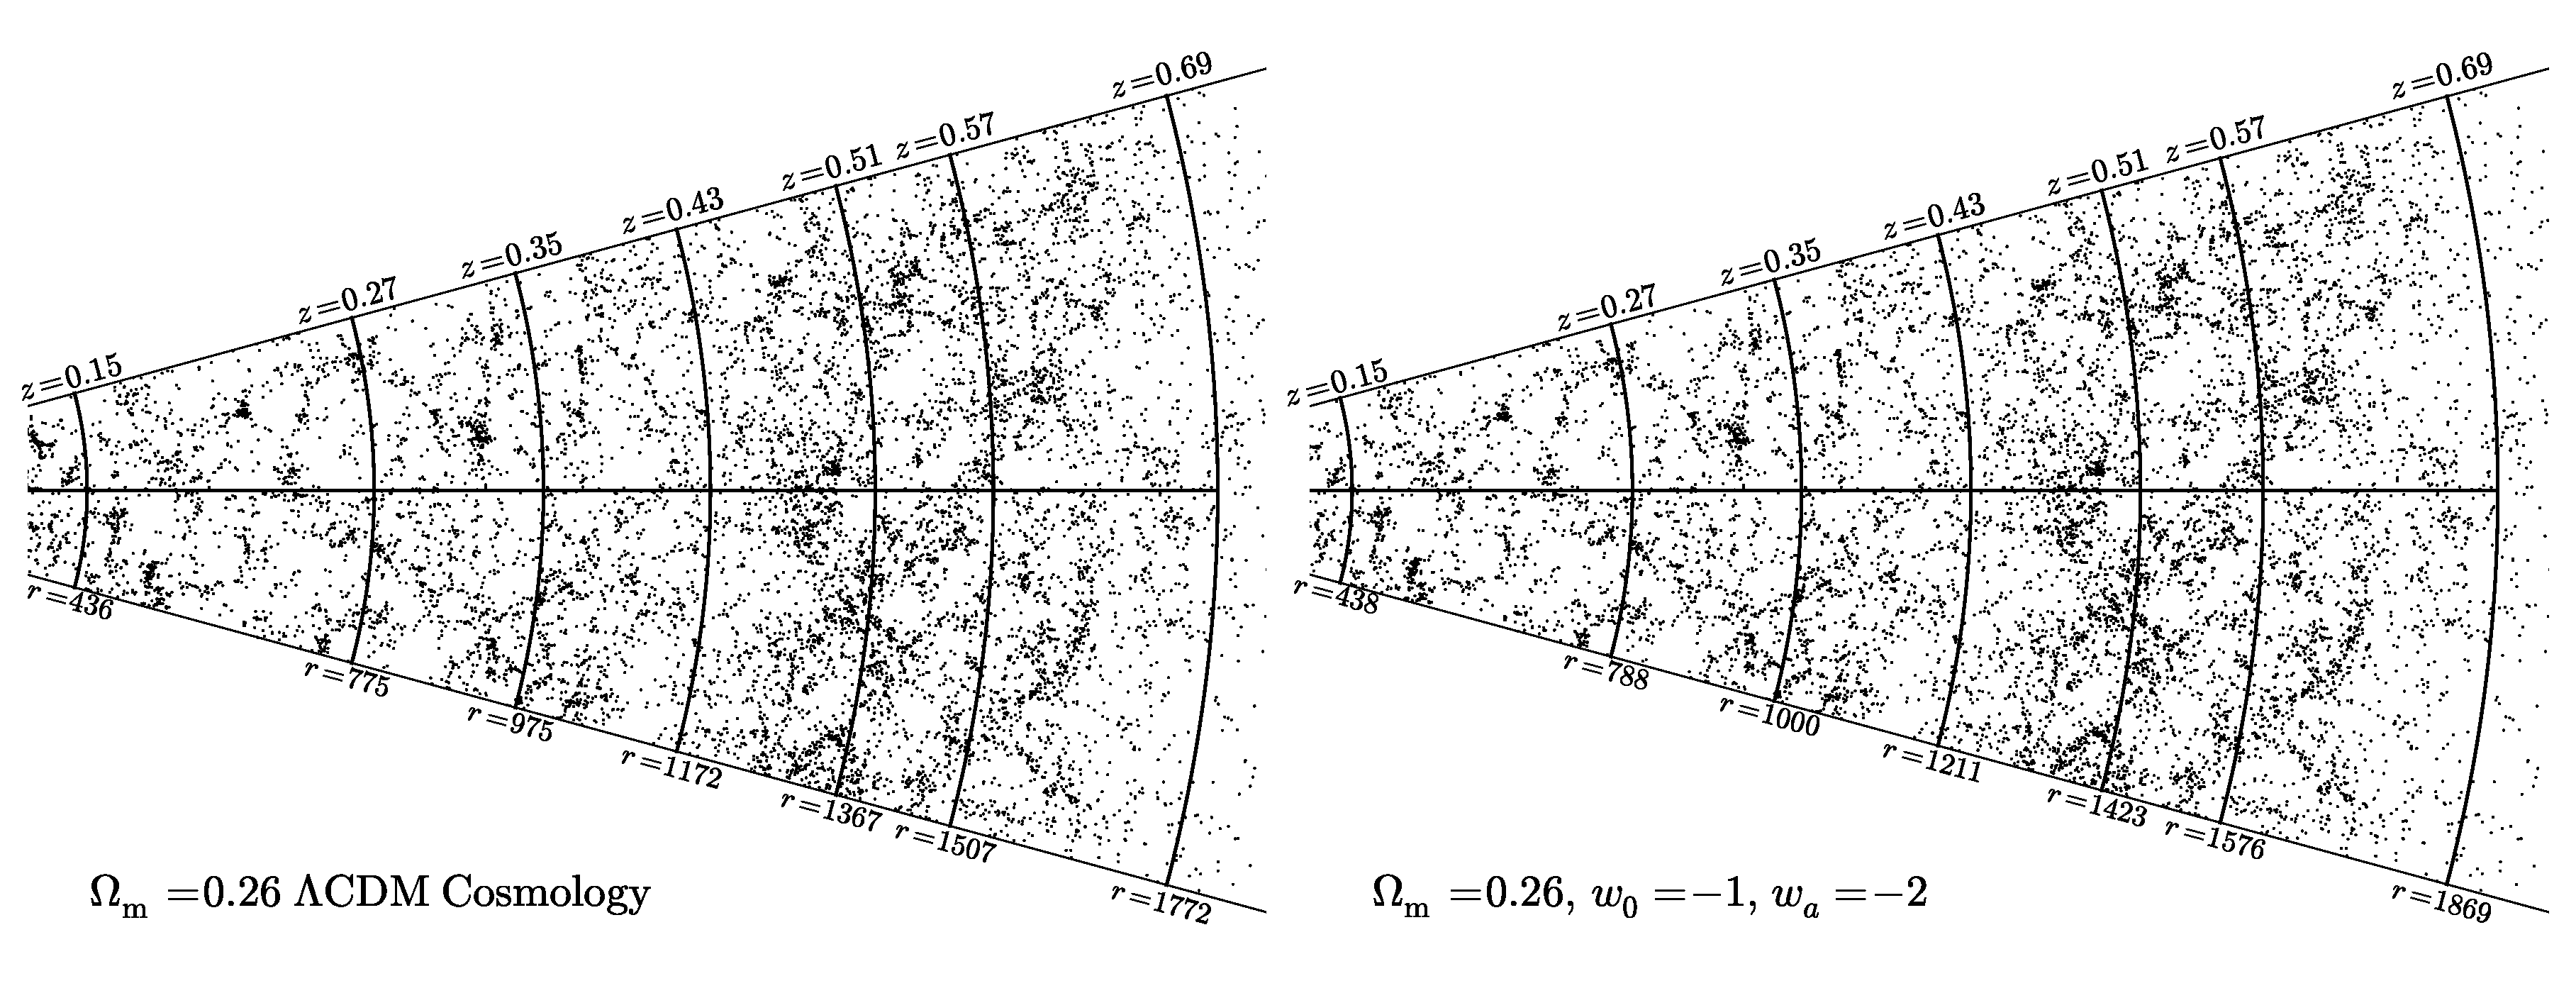
\includegraphics[width=18cm]{fig_fan.eps}
   %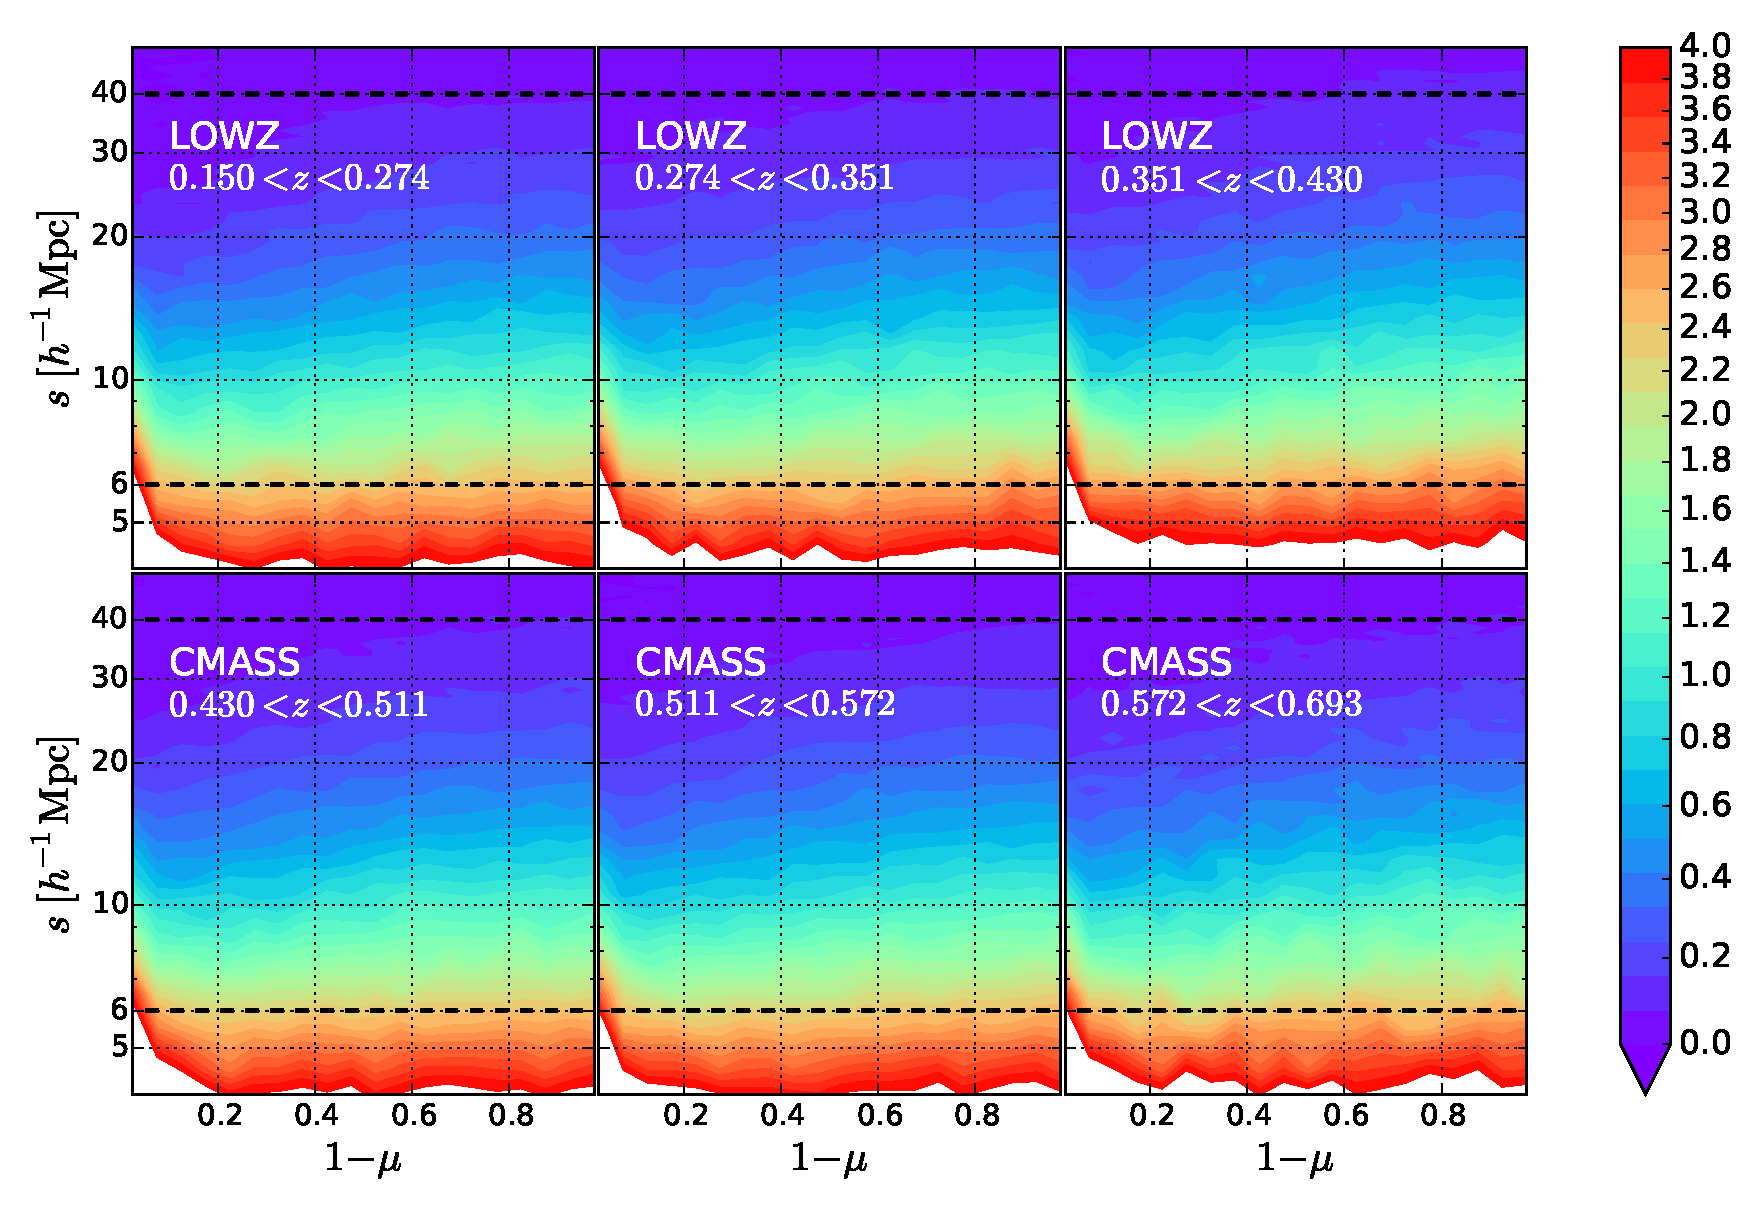
\includegraphics[width=9.0cm]{fig_2pcf.eps}
   %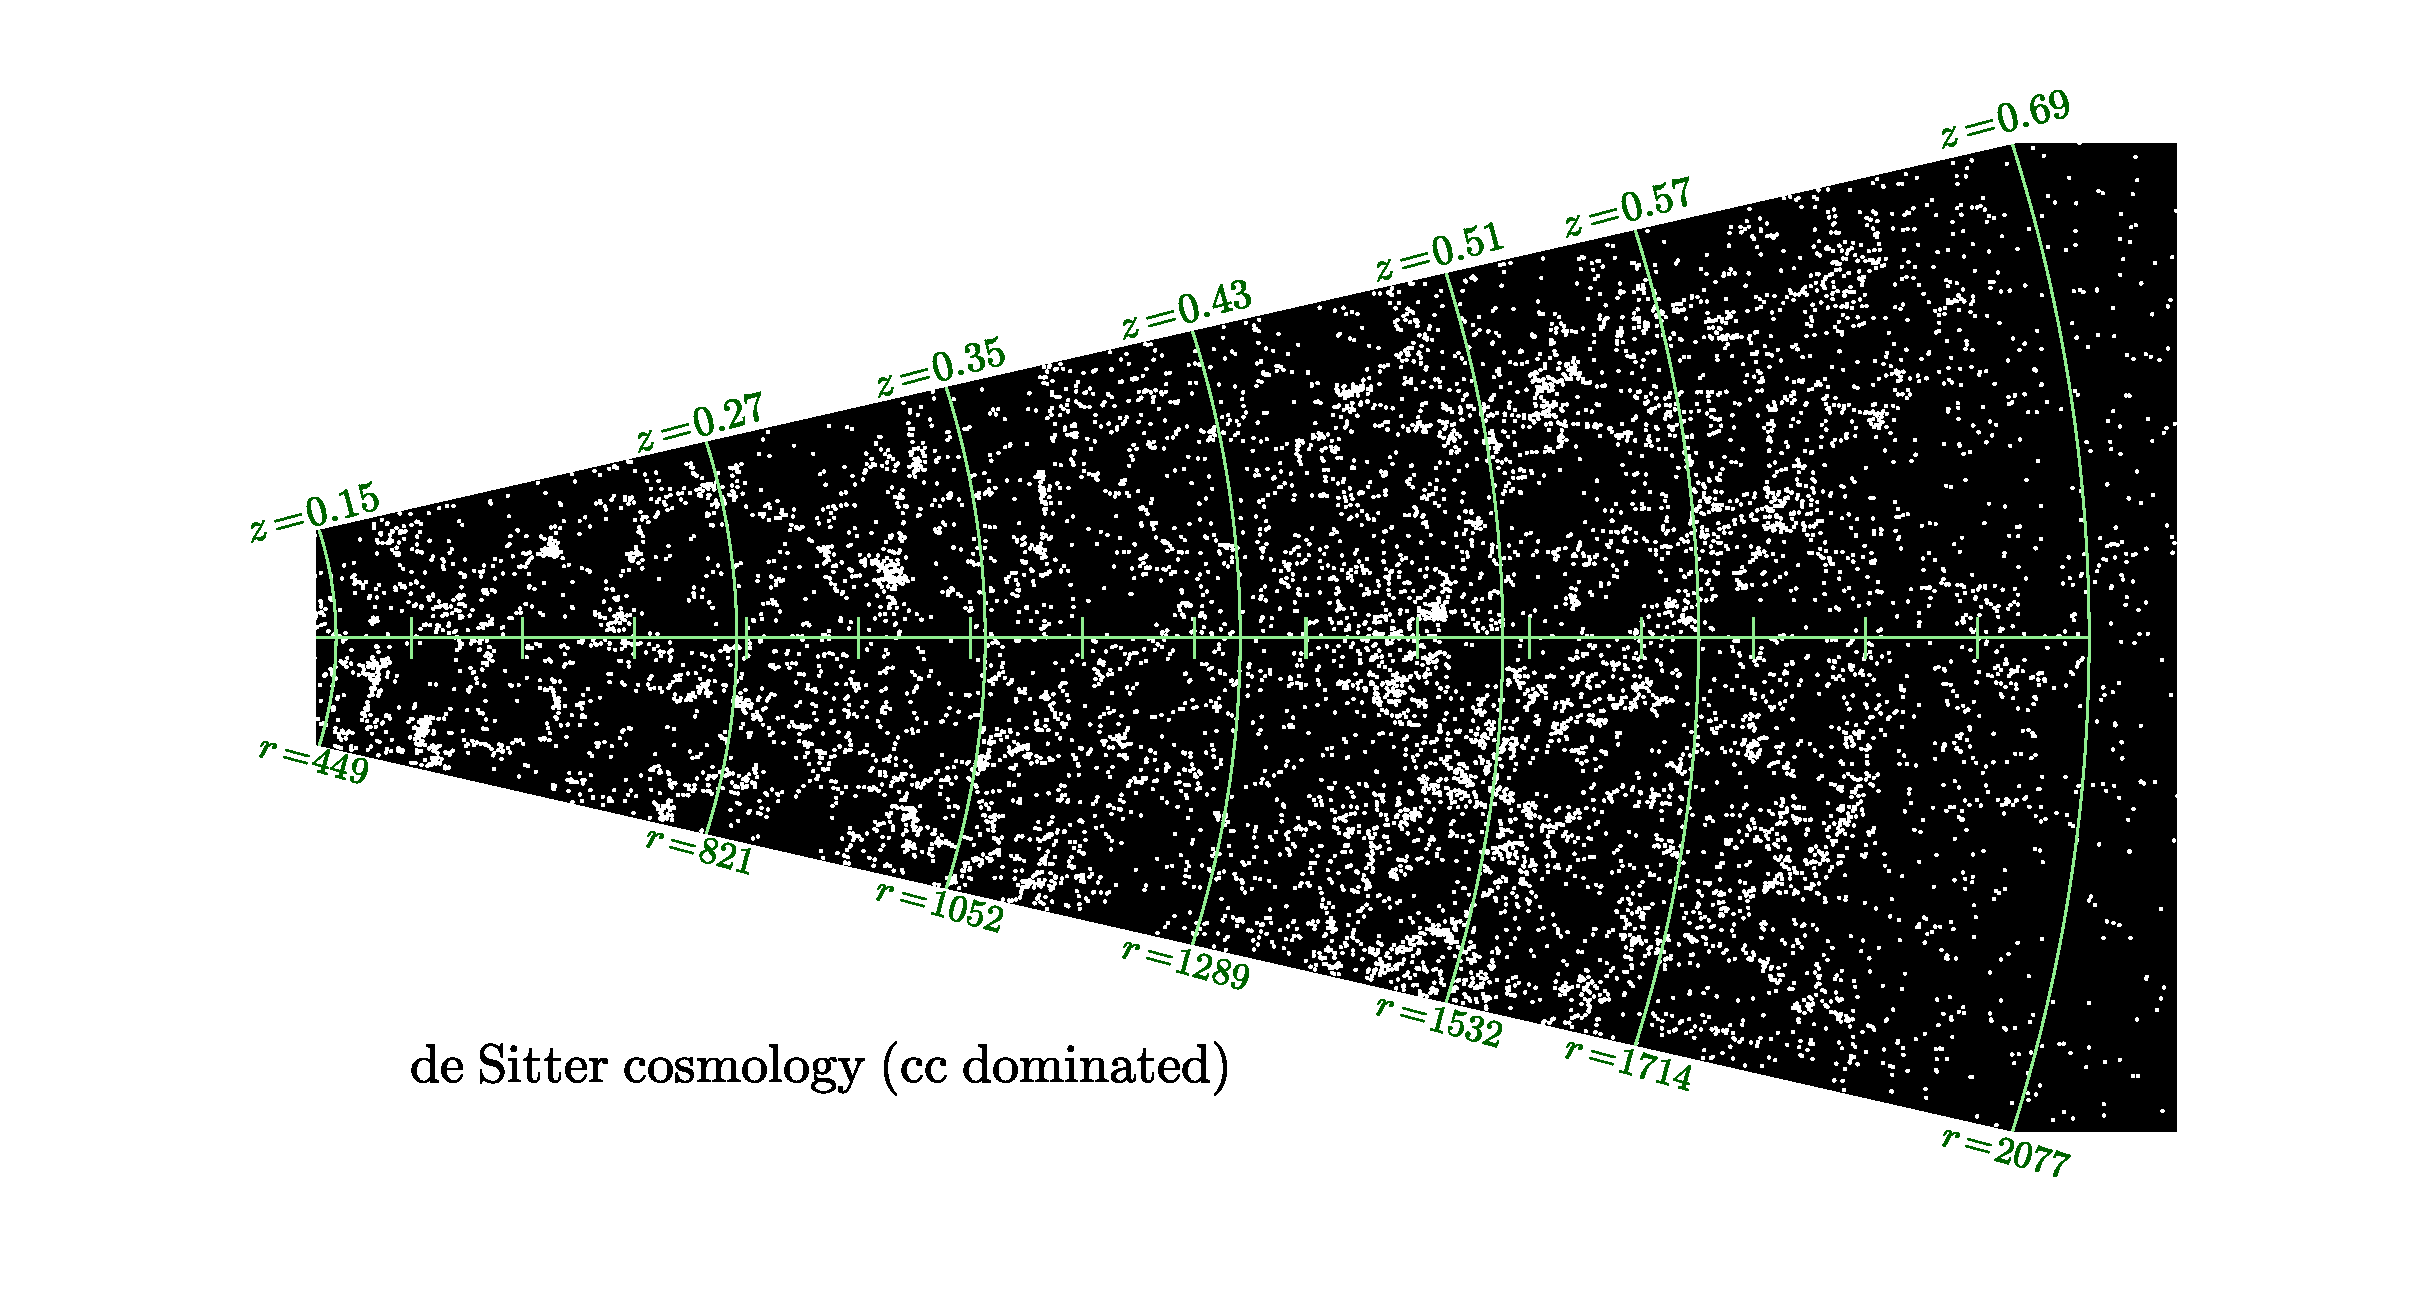
\includegraphics[width=8.5cm]{fig_fan_2.eps}
   }
   \caption{\label{fig_fan}
   %We split the BOSS DR12 galaxies into six redshift bins to measure the evolution of shape distortion.
   A patch of SDSS BOSS DR12 galaxies in the fan shape region of 
   $\rm 140^\circ < R.A. < 170 ^\circ$, $\rm 10^\circ < Decl. < 13 ^\circ$,
   split into six non-overlapping redshift bins (marked by the light green arcs) in order to probe the redshift evolution of anisotropic clustering.
   In the left and right panels, we plot the galaxy positions computed in two cosmologies: the $\Omega_m$=0.26 $\Lambda$CDM, 
   and a dynamical dark energy cosmology with $\Omega_m=0.26,\ w_0=-1,\ w_a=-2$.
   Redshifts and comoving distances (in unit of $h^{-1}\rm Mpc$) of the edges of redshift bins are listed.
   %The shape of structures look different in these two cosmologies. 
   In the dynamical dark energy cosmology, we see relative stretch of structures compared with the $\Lambda$CDM cosmology.
   The stretch is not significant in the first redshift bin, and becomes large in high redshift bins.
   We use this apparent distortion to discover the AP effect and place constraints on cosmologies.
   %By investigating how the anosotropy of galaxy distribution evolves in the six redshift bins,
   %we are able to distinguish different cosmologies.
   %The obtained galaxy distribution is different.
   %
   %The blue and green solid histograms show the redshift density distribution of LOWZ and CMASS galaxies in the $\Omega_m=0.31$ $\Lambda$CDM. 
   %The vertical dashed lines define the six redshift bins that are used to cut the samples.
   %The number of LOWZ/CMASS galaxies in the three low/high redshift bins are listed.
   %Right panel: 2D contour map of measured $\xi$ as a function of $\mu$ and $s$, from the six redshift bins of LOWZ and CMASS samples, 
   %   in the cosmology of $\Omega_m=0.31$ $\Lambda$CDM model.
   % The black dashed lines mark the clustering region 6-40\ Mpc/h studied in the AP method.
   % The six contour maps have rather similar appearance, implying small redshift evolution of $\xi$ from RSD.
   }
\end{figure*}


The  origin  of  the late-time accelerating  expansion  of  the  universe  is  one of  the  most  salient  questions  in  contemporary cosmology. 
Theoretical explanations for this phenomena are numerous and range from a non-zero  vacuum energy, an evolving  scalar  field  remnant  from  the  big  bang, 
to modifications of Einstein's General Relativity \citep{Li2011,2012IJMPD..2130002Y}. 
Considering the wealth of theoretical explanations, 
it is crucial to obtain precise and unbiased measurements of the expansion history of the Universe which allows us to 
differentiate between competing models. 

In recent years the Alcock-Paczynski (AP) test \citep{AP1979} applied to galaxy redshift samples \citep{Outram2004,Blake2011,Alam2016}, 
has allowed tight constraints to be placed on the background averaged distance scales, $D_A(z)$ and $H^{-1}(z)$.  
Assuming an incorrect cosmological model for the coordinate transformation between redshift space and comoving space
produces residual geometric distortions in the resultant galaxy distribution (see Figure \ref{fig_xy}). 
These distortions are induced by the fact that measured distances along 
and perpendicular to the line of sight depend on the given cosmological parameters. 
Therefore, measuring the ratio of galaxy clustering in the radial and transverse directions provides a probe of this AP effect.

%The BAO standard ruler method for obtaining estimates of $D_A(z)$ and $H^{-1}(z)$ is widely used and accepted by the community.
%However, since these measurements are made on large scales (~$120$Mpc), 
%they require large comoving volumes and wide redshift bins to reduce cosmic variance. 
%This results in estimates of the cosmic observables at fewer redshifts and with access to fewer Fourier modes. 
%This reduction of information hinders our attempts to test dark energy models. 

The main caveat in applying the AP test is that 
the radial distances of galaxies are inferred from observed redshifts.
Thus AP tests are inevitably affected by the peculiar motions of galaxies,
which leads to apparent anisotropy in the clustering signal, even if the adopted cosmology is correct.
The effect, known as redshift-space distortions (RSD),
is notoriously difficult to model accurately in the statistics of galaxy clustering \citep{Ballinger1996}.

The symmetry properties of galaxy pairs \citep{Marinoni2010}  could also be used to probe the AP effect;
however, since the peculiar velocity distorts the redshifts and changes the apparent tilt angles of galaxy pairs,
this method is also seriously limited by RSD \citep{Jennings2011}.



In an effort to minimize RSD contamination, the shape of void regions \citep{Ryden1995,LavausWandelt1995}  has been 
proposed as an AP probe. This approach has the advantage that the void regions are easier to model compared with dense regions, 
but has limitations in that it utilizes only low density regions of the LSS and requires large samples to attain statistical significances and achieve competitive constraints \citep{Qingqing2016}.

%In an effort to overcome the RSD problem, 
%\citep{Li2016} proposed to apply the AP effect to clustering on small scales. 
%However, redshift space distortions affect the angular clustering of galaxies, mimicking a signal similar to the AP effect, 
%thus contaminating the cosmological information.

Previously, we proposed to use the {\it redshift dependence} of the AP distortion \citep{Li2014} as a way of mitigating the RSD effect. 
The clustering anisotropies produced by RSD are, although large, close to uniform in magnitude over a wide range in redshift.  
However, if cosmological parameters are incorrectly chosen and there exists the AP effect, 
the anisotropy in the clustering signal has a clear redshift dependence
(as an illustration, Figure \ref{fig_xy} shows how the shape distortion varies with distance 
when incorrect cosmologies are used to infer distance from redshift).
In \cite{Li2015}, we developed an AP methodology 
that utilizes the redshift dependence of the galaxy 2-point correlation function (2PCF), 
measured as a function of angle between the galaxy pair and line-of-sight (LoS).



\begin{figure*}
   \centering{
   %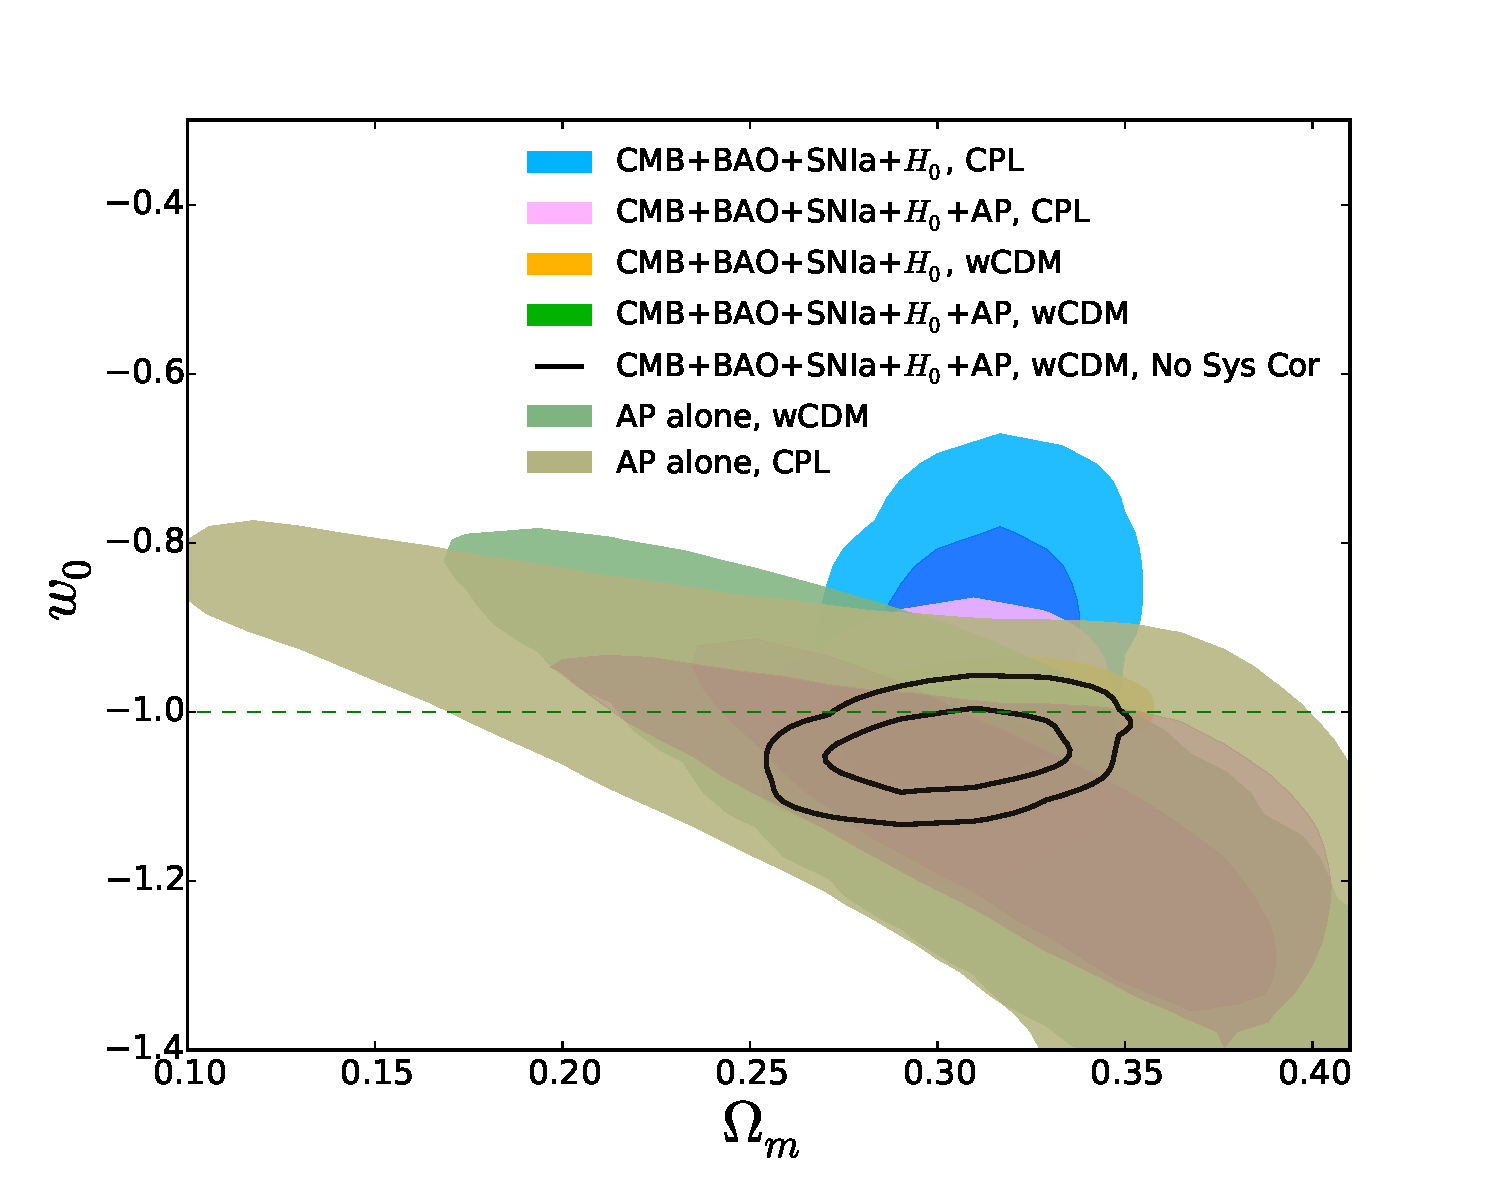
\includegraphics[width=9cm,natwidth=4,natheight=4]{figCPL_a.pdf}
   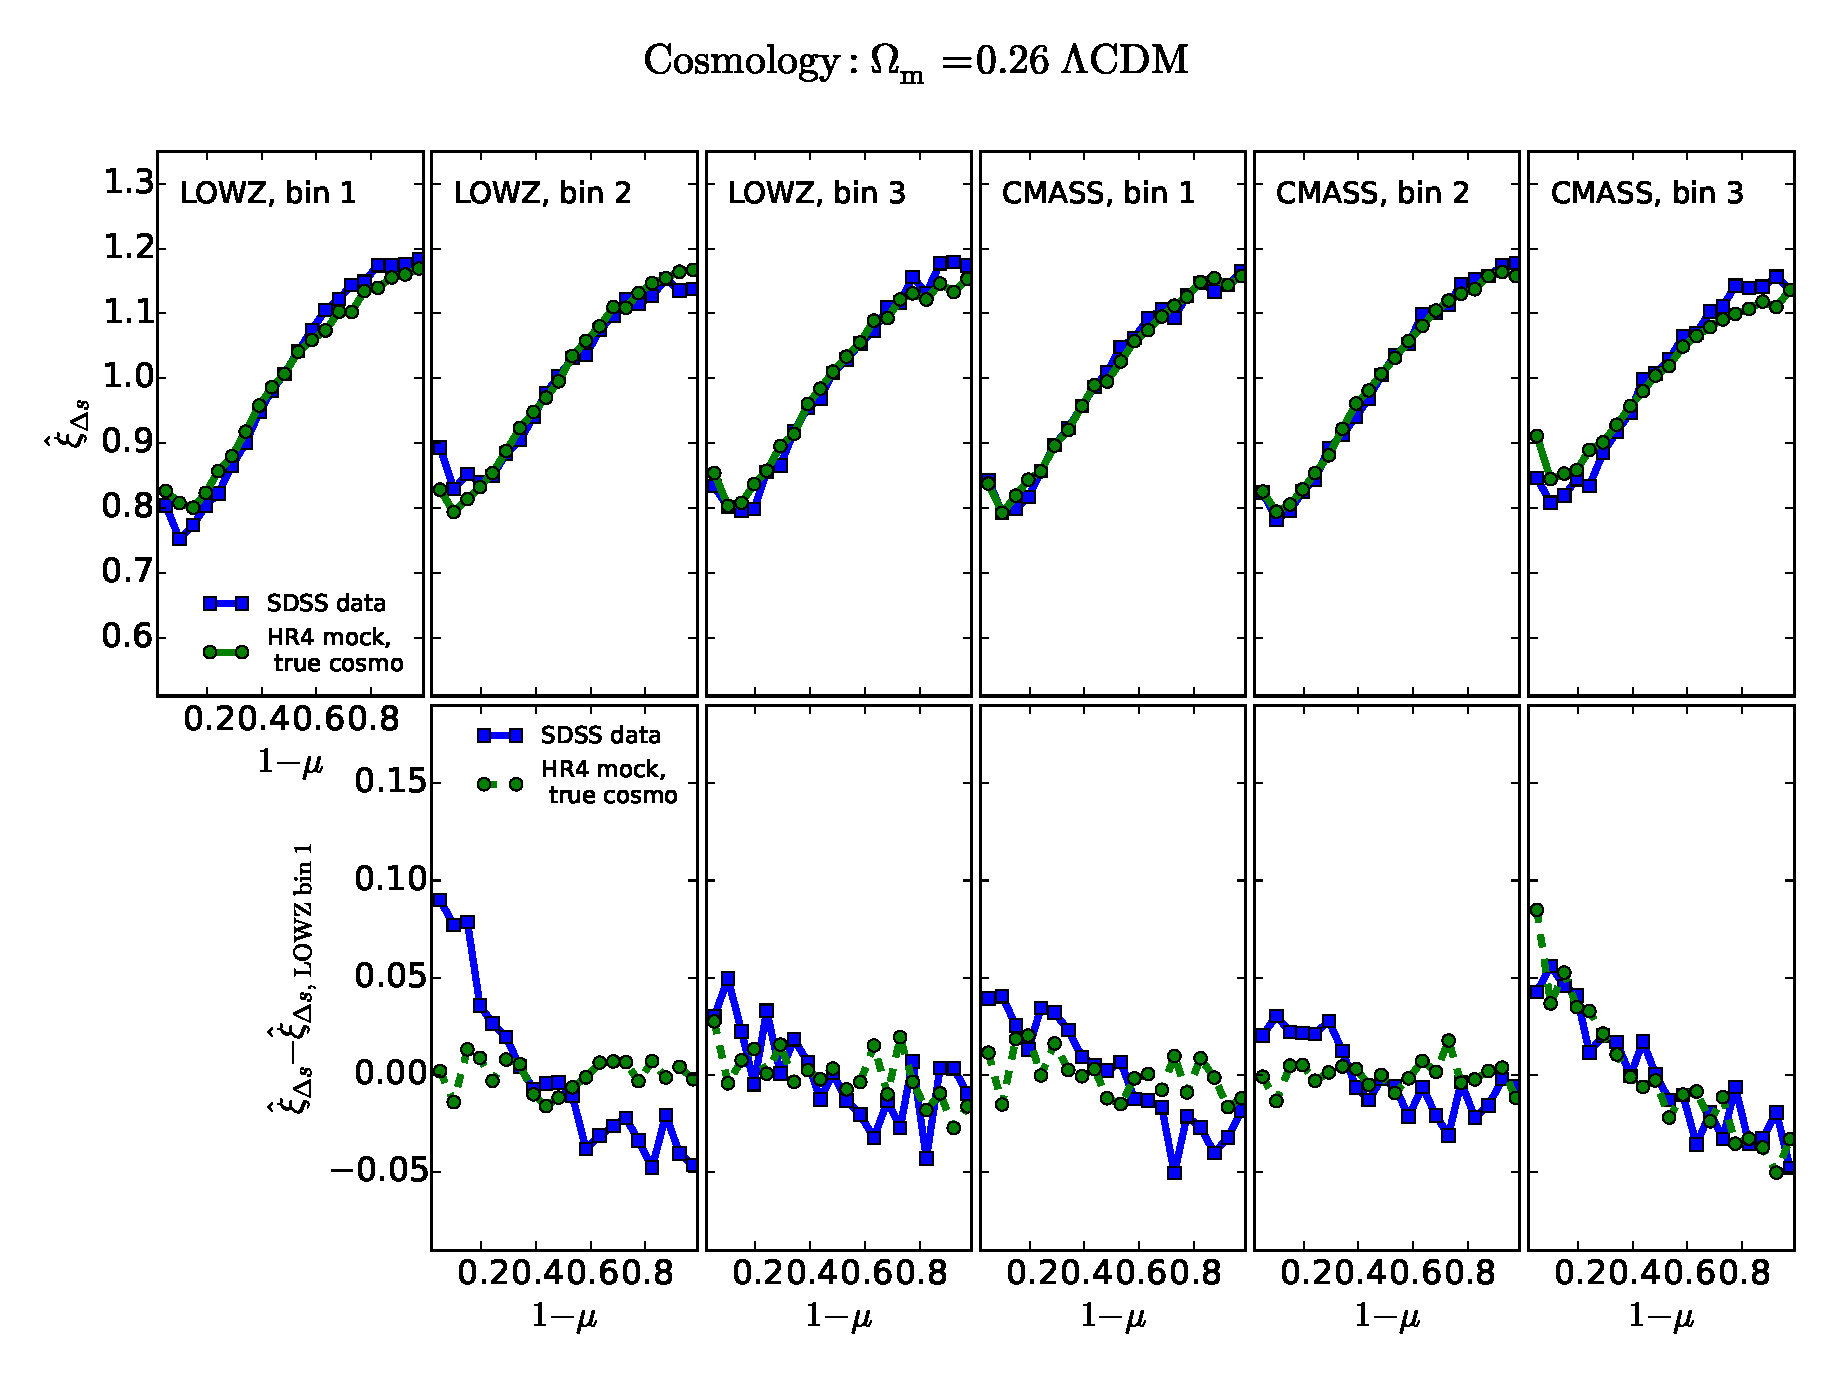
\includegraphics[width=8.95cm]{fig_xi_cosmo1.eps}
   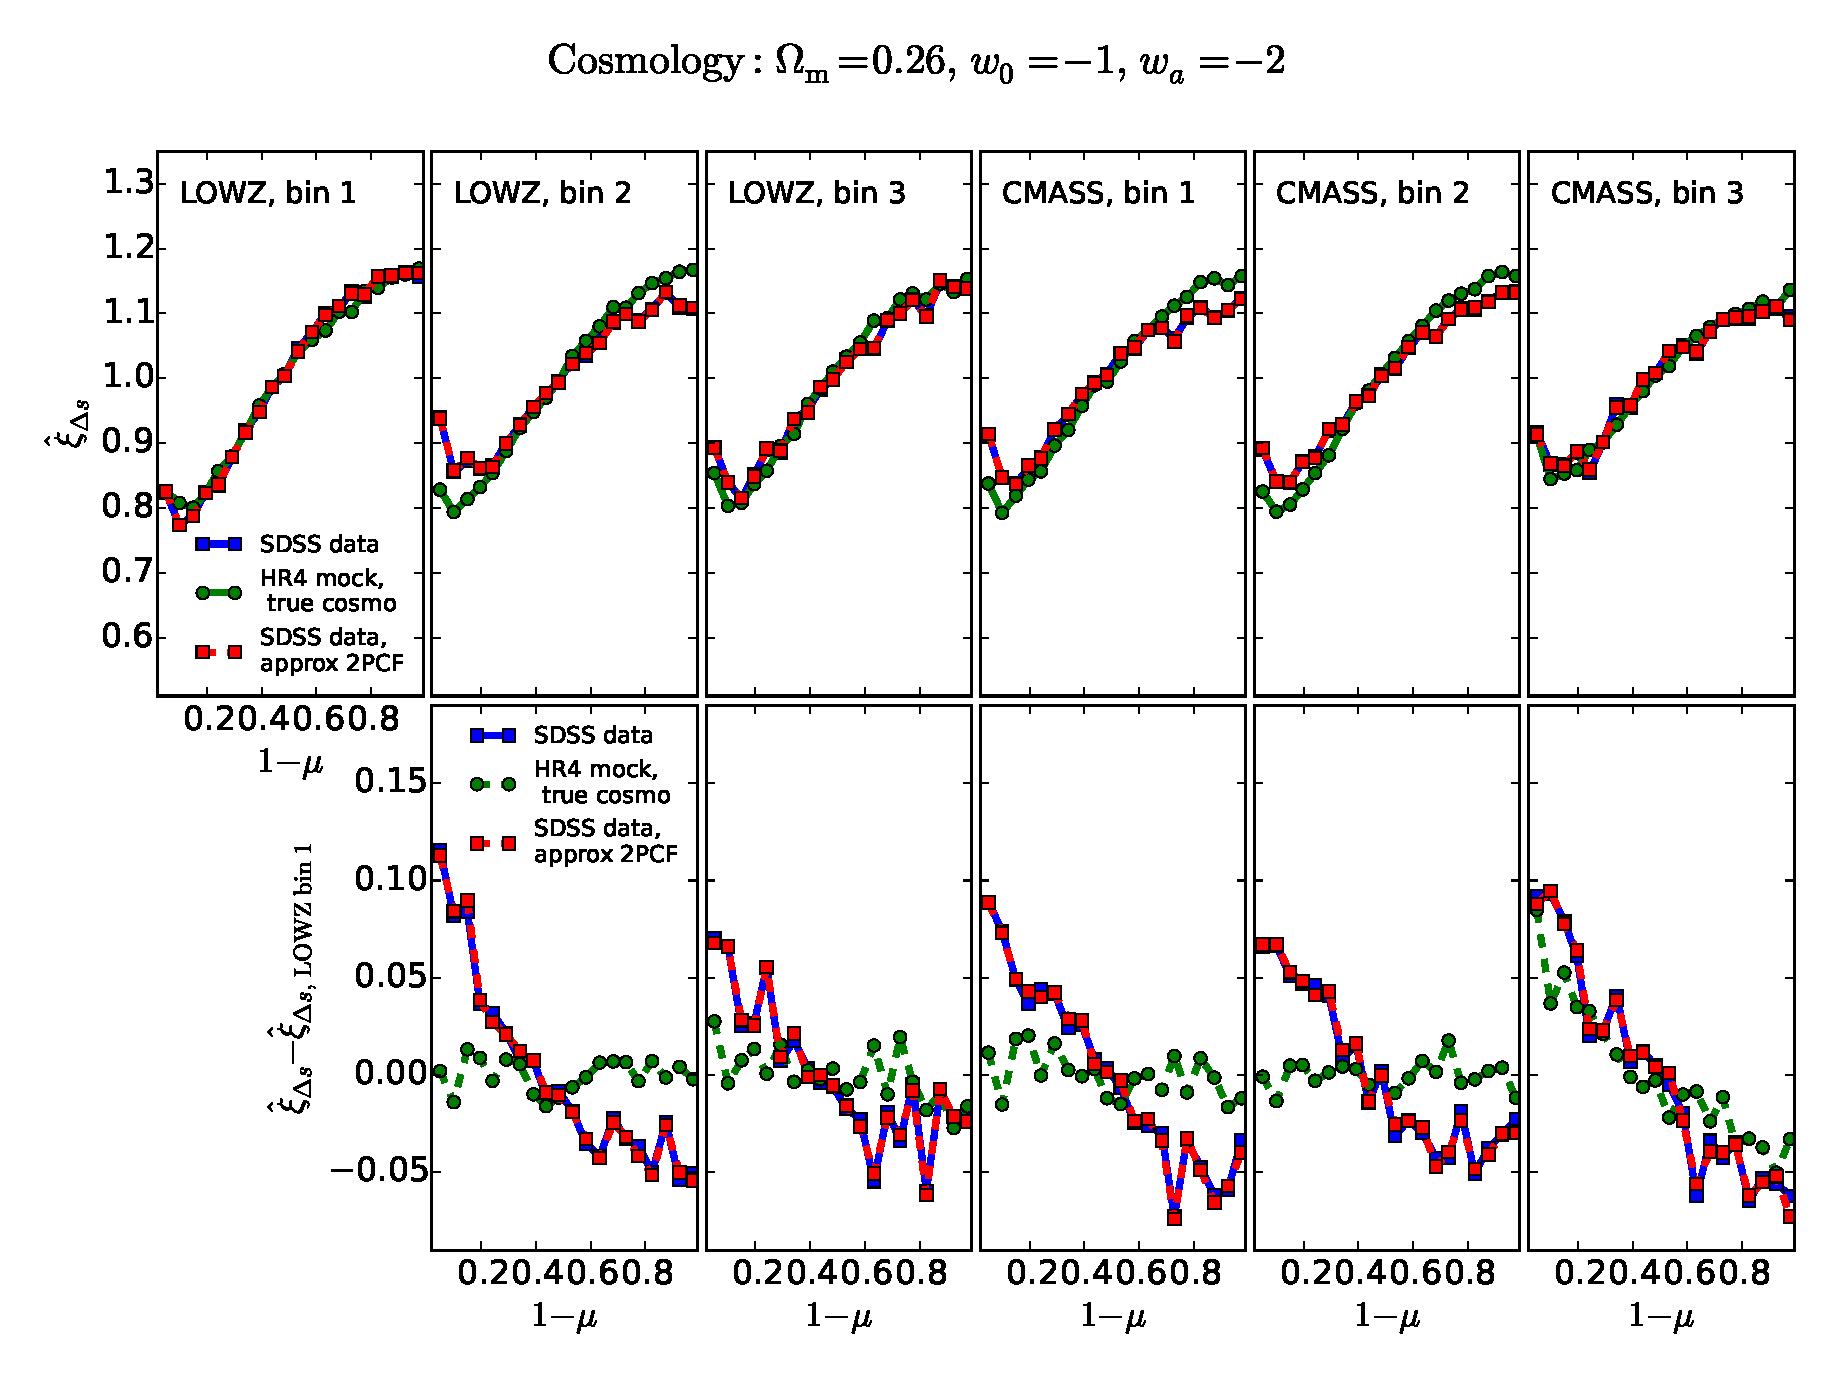
\includegraphics[width=8.95cm]{fig_xi_cosmo2.eps}
   }
   \caption{\label{fig_xi}
   $\hat\xi_{\Delta s}(\mu)$ measured from the SDSS BOSS DR12 galaxies in six redshift bins (three in LOWZ and three in CMASS),
   assuming the $\Omega_m=0.26$ $\Lambda$CDM cosmology and a more dark energy dominated cosmology, $\Omega_m=$0.11 $\Lambda$CDM.
   Measurements in the six redshift bins and their redshift evolution with respective to the first bin of LOWZ are plotted.
   In the $\Omega_m$=0.11 cosmology, the shapes of $\hat\xi_{\Delta s}(\mu)$ are different from the $\Omega_m=0.26$ cosmology results,
   and the difference changes with redshift;
   a large redshift evolution of $\hat\xi_{\Delta s}(\mu)$ is detected in this cosmology, 
   indicating that it is not likely to be the underlying true cosmology of our universe.
   The measurements in the HR4 mock catalogues (always in the $\Omega_m=0.26$ $\Lambda$CDM cosmology; plotted in green color)
   match the shape of curves measured from observational data, 
   indicating that the simulation well reproduces the FoG and Kaiser effects.
   For the $\Omega_m$=0.11 cosmology, we also plot the approximate 2PCFs (red dashed lines) 
   inferred using the technique described in Sec. \ref{sec:approx_2pcf}.
   The error induced in the approximation procedure is very small.
   }
\end{figure*}


In an earlier work (Li et al. 2016, hereafter L16) we applied this AP method to galaxies from the 3rd incarnation of the Sloan Digital Sky Survey (SDSS-III). 
Combining the method with measurements of the Cosmic Microwave Background (CMB), type Ia supernovae (SNIa), 
baryon acoustic oscillations (BAO), and $H_0$,
we obtained very tight constraints of $ \Omega_m = 0.301 \pm 0.006,\ w=-1.054 \pm 0.025$.
In reducing the RSD effect, 
we were able to use galaxy clustering on scales down to 6 $h^{-1}$Mpc,
which is a major advance in extracting cosmological information 
on small scales where galaxy clustering is strong and many independent structures exist.



In this paper, we continue to develop our previous methodology and proceed to set the constraints on dynamical dark energy. 
We will present an improved methodology compared to L16, 
allowing for faster likelihood estimation and thus the exploration of larger, higher dimensional parameter spaces. 
The methodology we will present here, can be applied to any model of dynamical dark energy, 
or indeed any appropriately chosen parametric or non-parametric decomposition of the cosmic expansion history. 
However, as a first step, in this paper we will focus on the widely used Chevallier-Polarski-Linder (CPL) parametrization\citep{CPL_CP,CPL_L},
\begin{equation}
w(z) = w_0 + w_a (1-a) = w_0 + w_a \frac{z}{1+z}.
\end{equation}
This parametrization characterizes the dark energy equation-of-state (EoS) by two free parameters;
$w_0$ determines the present-day value, while parameter $w_a$ characterizes the first-order derivative of $w$ with respect to $a$. 
The possible redshift evolution of dark energy EoS is not considered in the analysis of L16. 

The CPL parametrization has many obvious advantages, for instance, a manageable parameter space, 
the bounded behavior at high redshift, 
and the ability to accurately reconstruct many dark energy theories \citep{CPL_L}. 
%So it was widely used in the literature to reconstruct dark energy from observations.
The constraining power is usually quantified by the DETF  \citep[Dark Energy Task Force;][]{DETF} figure of merit, 
defined as the reciprocal of the area of the error ellipse enclosing the 95\% confidence limit (CL) in the $w_0 - w_a$ plane. 

Figure \ref{fig_xy} illustrates the AP effect in wrong cosmologies.
A redshift dependence of shape distortion is observed in case of adopting wrong values of $w_0$ and $w_a$,
thus we expect that these two parameters will be effectively constrained by our method.
There is a fare degree of degeneracy in the resulting expansion history
between increasing $w_0$ and adopting similar $w_0$ but increased $w_1$.

%{\bf AMTB: Please chose one kind of tense of verbs. It changes from sentences to sentences!}
%{\bf AMTB: How many mock BOSS samples are made from HR4?}



\section{Methodology}

\subsection{Quantifying the redshift dependence of the AP distortion}

The spectroscopic galaxy sample of SDSS-III BOSS (Baryon Oscillation Spectroscopic Survey) has two primary catalogues:
%the LOWZ at $z\leq0.4$, and CMASS covering $0.4\leq z \leq 0.7$. %of galaxies.
the LOWZ sample, designed as an extension of the SDSS-I/II luminous red galaxy sample to $z\approx 0.4$ and fainter luminosities,
and the CMASS sample covering a higher range ($0.4\lesssim z \lesssim 0.7$),
and made to be an approximately stellar mass limited sample of massive, luminous galaxies \citep{Reidetal:2016}.
In the clustering analysis we use 1,133,326 galaxies, split into six, non-overlapping redshift bins, 
$0.150<z_1<0.274<z_2<0.351<z_3<0.430<z_4<0.511<z_5<0.572<z_6<0.693$.
The edges are determined so that the number of galaxies are roughly the same in different redshift bins 
(for LOWZ and CMASS samples, respectively).

%The number density of galaxies and the redshift binning scheme is plotted in the left panel of Figure \ref{fig_TpCF}.

Figure \ref{fig_fan} shows a patch of 10,976 BOSS DR12 galaxies,
whose positions are computed in the $\Omega_m$=0.26 $\Lambda$CDM cosmology 
and a dynamical dark energy cosmology with $\Omega_m=0.26,\ w_0=-1,\ w_a=-2$.
The shape of structures look different in these two cosmologies. 
In the latter cosmology, there is apparent stretch of structures, 
and the degree of compression becomes more significant in higher redshift bins.
By investigating how the anisotropy of galaxy distribution evolves in the six redshift bins,
we are able to distinguish this cosmology from the $\Lambda$CDM cosmology.


Following our previous methodology, the information of anisotropic clustering is computed as 
%\footnote{These correlations were computed using the public code \texttt{KSTAT} \citep{kstat}.} 
\begin{equation}
\xi_{\Delta s} (\mu) \equiv \int_{s_{\rm min}}^{s_{\rm max}} \xi (s,\mu)\ ds,
\end{equation}
with $s_{\rm min}=6 h^{-1} {\rm Mpc},$ and $s_{\rm max}=40 h^{-1} {\rm Mpc}$.
We then normalize these {\em clustering shells} as 
\begin{equation}
\hat\xi_{\Delta s}(\mu) \equiv \frac{\xi_{\Delta s}(\mu)}{\int_{0}^{\mu_{\rm max}}\xi_{\Delta s}(\mu)\ d\mu}
\end{equation}
to nullify the amplitude information of the clustering signal, 
which is not associated with the AP test and is mostly sensitive to the galaxy bias evolution.
%The right panel of Figure \ref{fig_TpCF} shows the contour map of $\xi(s,\mu)$ measured in the six redshift bins.
%The contour lines are not horizontal due to the effects of peculiar velocity,
%and the RSD effect clearly manifest itself through the tilting of contour lines.
%However, the shape of the tilted lines remain similar at different redshifts, a fact that enables us  to mitigate the RSD effect by focusing on the redshift dependence of the anisotropic clustering signal.
The ``correct'' cosmological model is selected by minimizing the amount of redshift evolution of $\hat\xi_{\Delta s}$,
via a $\chi^2$ function of 
\begin{equation}
 \chi^2\equiv \sum_{i=2}^{6} \sum_{j_1=1}^{n_{\mu}} \sum_{j_2=1}^{n_{\mu}} {\bf p}(z_i,\mu_{j_1}) ({\bf Cov}_{i}^{-1})_{j_1,j_2}  {\bf p}(z_i,\mu_{j_2})
\end{equation}
where ${\bf p}(z_i,\mu_{j})$ is the redshift evolution of clustering with respect to the lowest redshift bin,
while subtracting systematic effects as
\begin{eqnarray}
 {\bf p}(z_i,\mu_{j}) \equiv\ & \left[\hat\xi_{\Delta s}(z_i,\mu_j)-\hat\xi_{\Delta s}(z_1,\mu_j)\right] \\ \nonumber
 &- \left[\hat\xi_{\Delta s}(z_i,\mu_j)-\hat\xi_{\Delta s}(z_1,\mu_j)\right]_{\rm sys}.
\end{eqnarray}
We use $n_{\mu}$=20, 21, ... 25 bins for the value of 
$0<\mu<\mu_{\rm max}$.
To reduce the fiber collision and the finger of god (FoG) effect \citep{FOG} near the LOS we take a cut $\mu_{\rm max} = 0.97$.

The systematics effects are estimated using mock catalogues drawn from Horizon Run 4 \citep[HR4;][]{HR4},
an N-body simulation with a box size of $L={3150}$ $h^{-1}$Mpc, the number of particles $6300^3$,   
initial redshift of $z_{i}=100$, and the WMAP5\citep{komatsu2011} cosmological parameters 
$(\Omega_{b},\Omega_{m},\Omega_\Lambda,h,\sigma_8,n_s)$  = (0.044, 0.26, 0.74, 0.72, 0.79, 0.96). 
Mock galaxy samples are produced using a modified version of the one-to-one correspondence scheme \citep{hong2016}. 
%As presented in \cite{Li2016}, the value of $\left[\hat\xi_{\Delta s}(z_i,\mu_j)-\hat\xi_{\Delta s}(z_1,\mu_j)\right]_{\rm sys}$
%(mainly comes from redshift evolution of RSD and galaxy bias)
%reaches 4 -- 6\% at the highest redshift bin,
%and is minor ($\lesssim2\%$) at the other redshift bins.


The covariance matrix, ${\bf Cov}$, is computed from the a set of 2,000 MultiDark PATCHY mock catalogues \citep{MDPATCHY}.
The statistical bias and scattering in the likelihood function (due to the finite number of mocks in covariance estimation) 
are adequately corrected \citep{Hartlap,Percival2014}.

The MultiDark PATCHY  mocks are produced using approximate gravity solvers and analytical-statistical biasing models.
They were calibrated to the BigMultiDark N-body simulation \citep{K2014}, which 
uses $3\,840^3$ particles in a volume of $(2.5h^{-1}\rm Gpc)^3$,
assuming a $\Lambda$CDM cosmology with 
$(\Omega_{b},\Omega_{m},h,\sigma_8,n_s)$  = (0.048206, 0.307115, 0.6777, 0.8288, 0.9611). 
%$\Omega_m = 0.307115$, $\Omega_b = 0.048206$, $\sigma_8 = 0.8288$, $n_s = 0.9611$, and $H_0 = 67.77 {\rm km}\ s^{-1} {\rm Mpc}^{-1}$.
The mock surveys can well reproduce the number density, 
selection function, survey geometry, and 2PCF measurement of the BOSS DR12 catalogues.
They have been adopted for statistical analysis of BOSS data in a series of works \citep[see][and references therein]{Alam2016}.




\begin{figure*}
   \centering{
   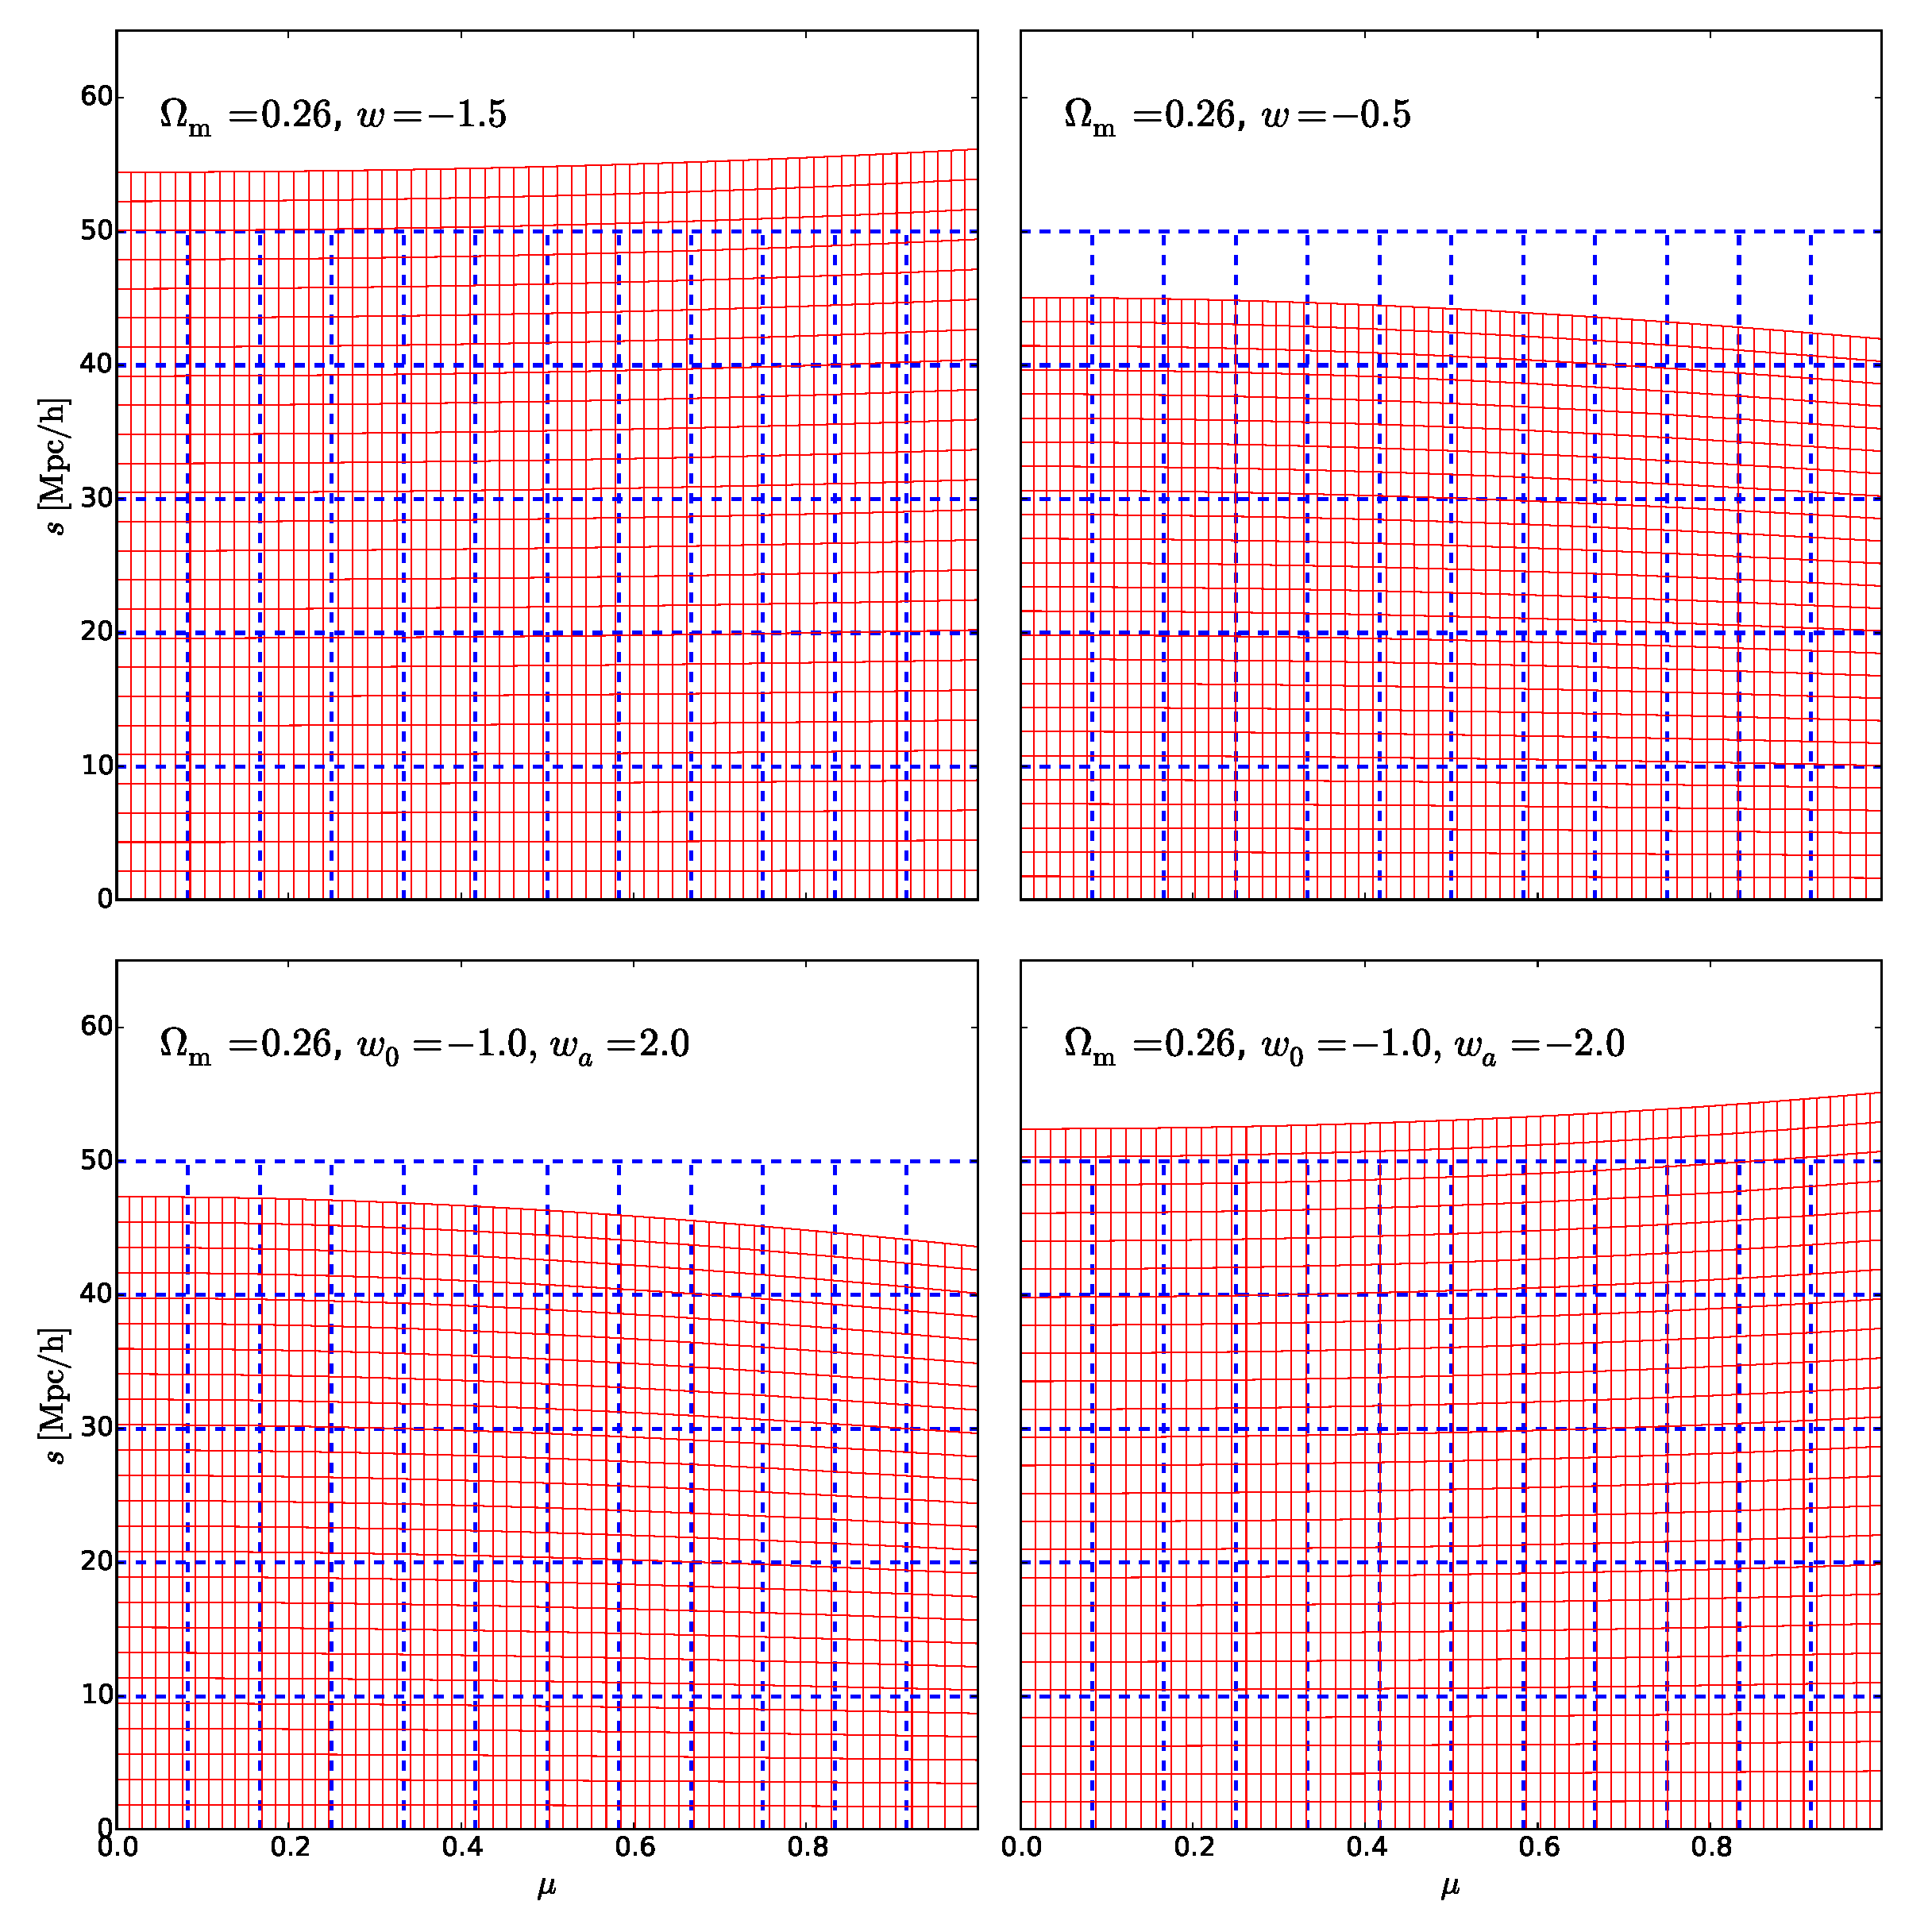
\includegraphics[width=12cm]{fig_smu.eps}
%   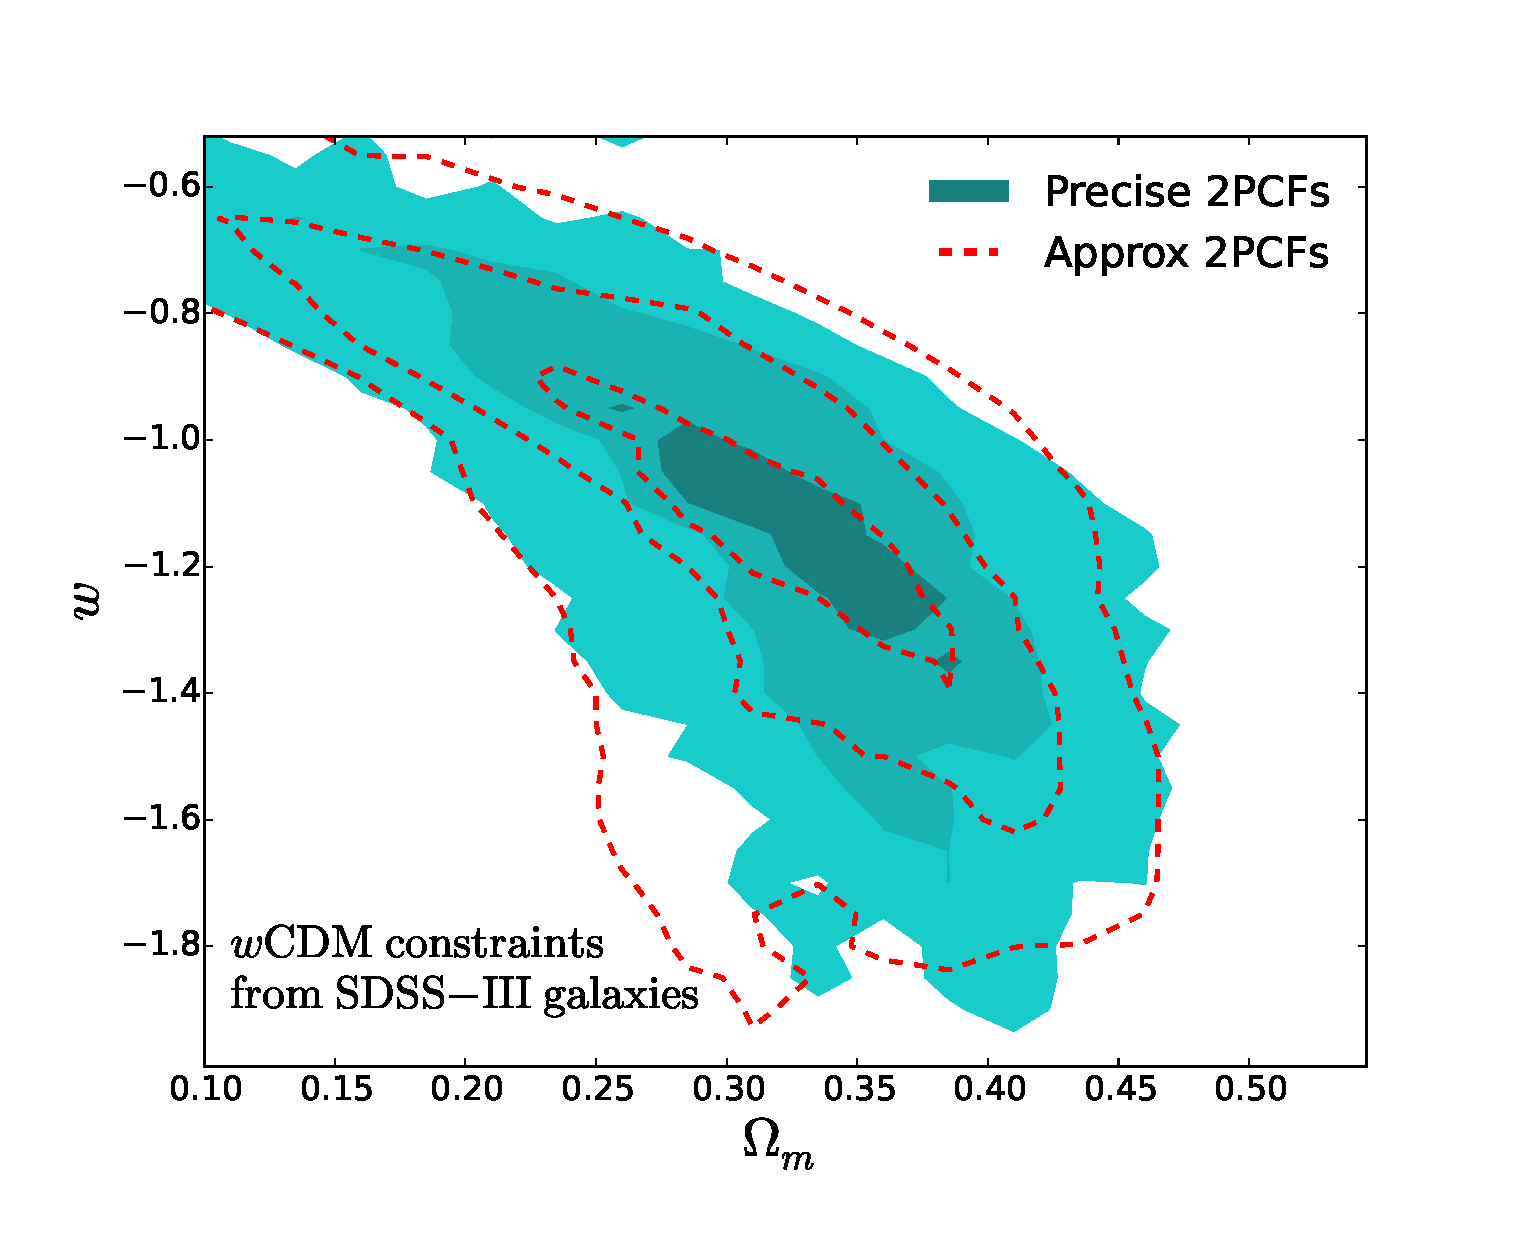
\includegraphics[width=10.5cm]{fig_comp.eps}
   }
   \caption{\label{fig_method}
 Mapping $\xi(s,\mu)$ from the fiducial cosmology (taken as the $\Omega_m=0.26$ $\Lambda$CDM cosmology) to four other cosmologies,
   $(w_0,w_a) = (-1.5,0),\ (-0.5,0),\ (-1,2)\ \rm and\ (-1,-2)$.
 The number counts are measured in the fiducial cosmology in the blue dashed grid;
 %In the four cosmologies,  %due to the distortion of geometry,
 in other cosmologies their distribution becomes the red solid grid (according to Equation \ref{eq:smumap}).
 We use this relation to obtain $\xi(s,\mu)$ in these non-fiducial cosmology without re-measuring the number counts.
 To enhance the accuracy, we count the number of galaxy pairs in 5 times smaller pixels (the small red pixels), 
 and group them together to infer the values of $\xi(s, \mu)$ in the blue dashed pixels
 (for illustration purpose, the blue and red grids are 10 times sparser than the grids adopted in the real analysis).
}
\end{figure*}

\begin{figure*}
   \centering{
   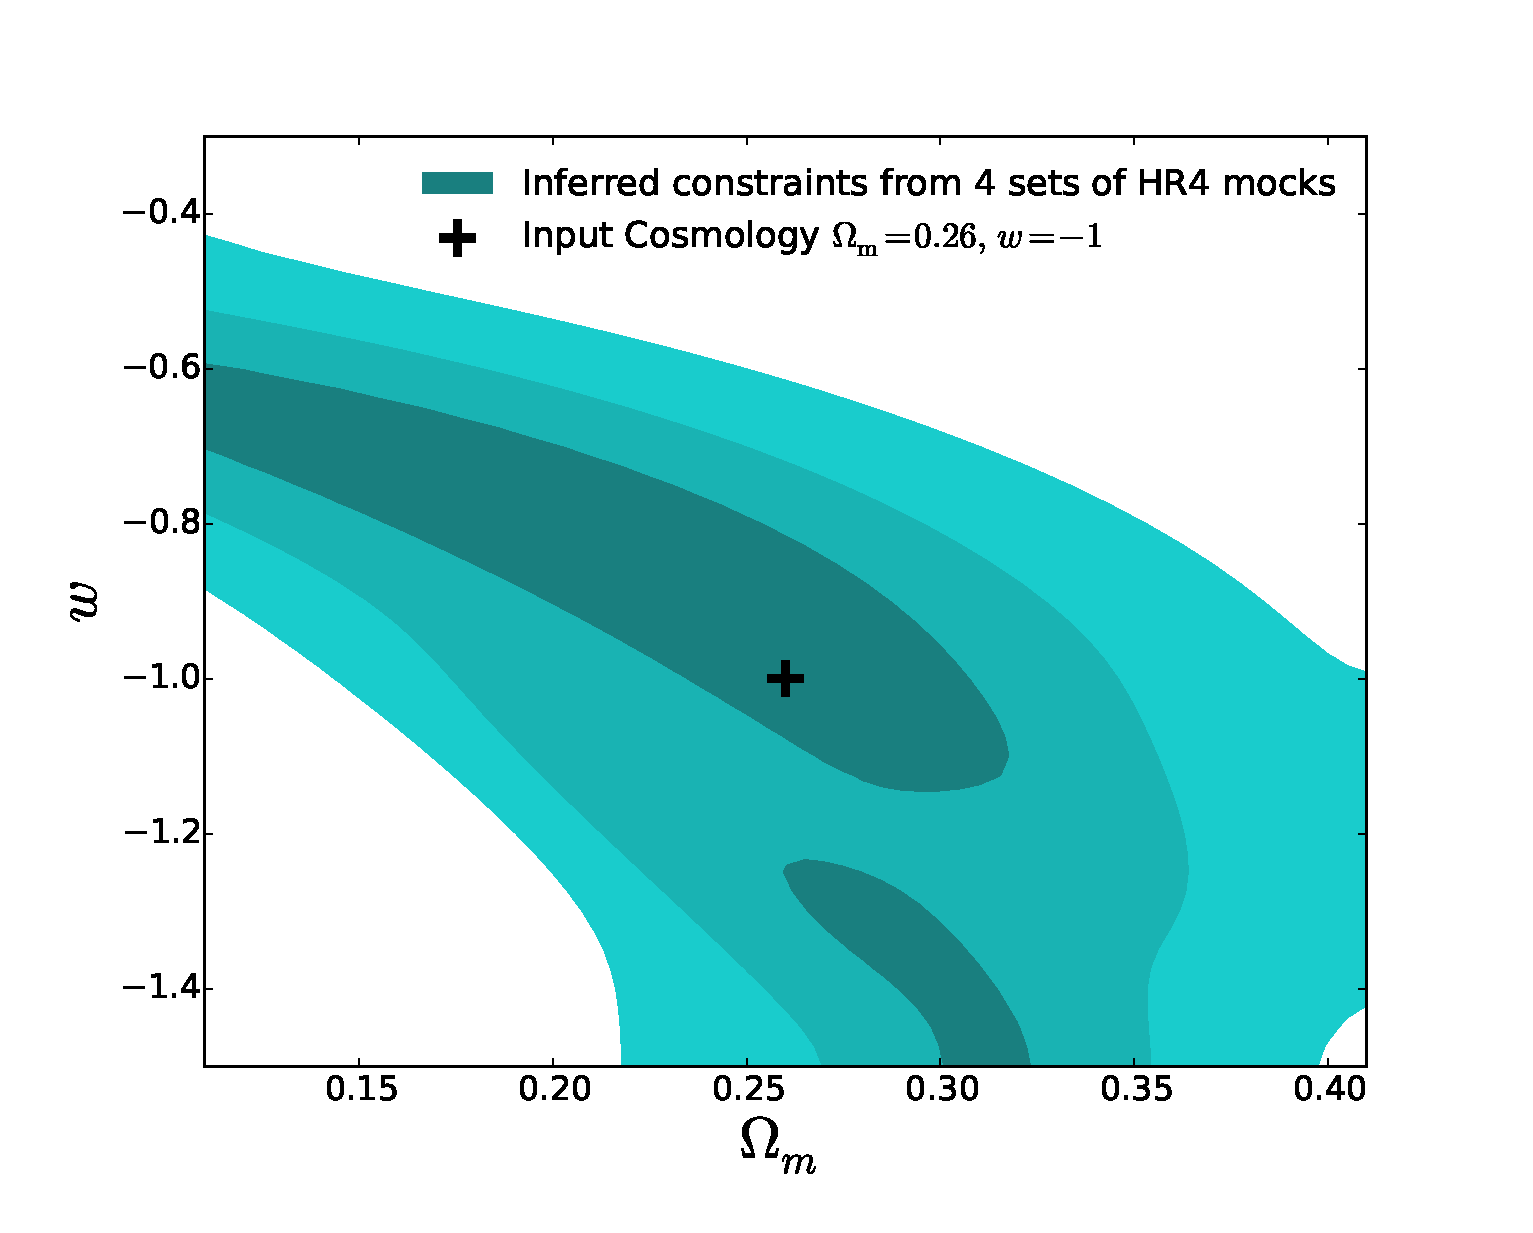
\includegraphics[width=8.5cm]{fig_IO.eps}
   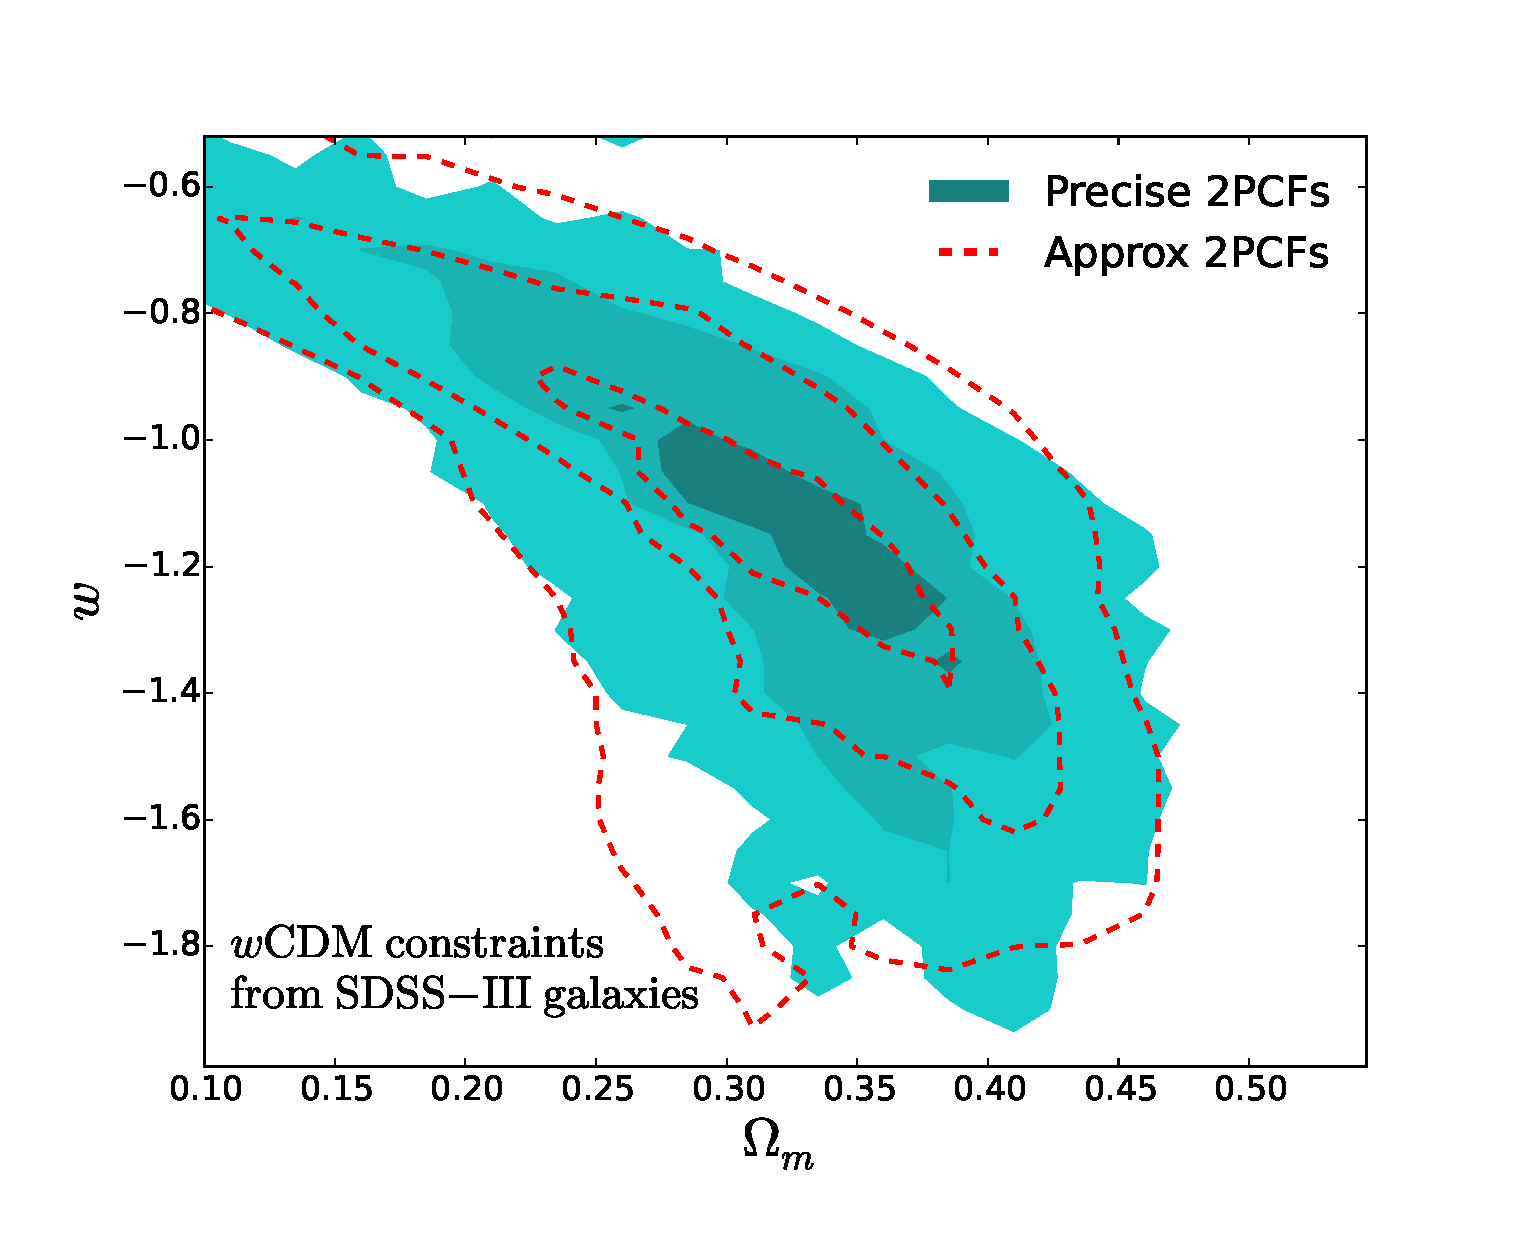
\includegraphics[width=8.5cm]{fig_comp.eps}
   }
   \caption{\label{fig_Check}
 Left panel: Input-output test of the AP methodology using four sets of BOSS DR12 galaxy mock catalogues constructed from the HR4 simulation.
 The approximate 2PCFs are adopted in the analysis.
 The inferred cosmological constraints from the method, shown in the cyan contours, are consistent with the input cosmology
 (the simulation cosmology, i.e. the $\Omega_m=0.26$ $\Lambda$CDM; marked by the black plus sign).
 Right panel: Cosmological constraints from the BOSS DR12 galaxies, assuming a $w$CDM cosmology 
 (i.e., the value of $w_a$ fixed as zero).
 Results obtained using the precise 2PCFs (cyan filled) 
 and approximate 2PCFs (red dashed) agree with each other quite well.
   }
\end{figure*}

{\bf TBA}
As an illustration,
Figure \ref{fig_xi} shows how we us the above procedure to distinguish different cosmologies.
Here we plot the value of $\hat\xi_{\Delta s}(\mu)$, as long as its redshift evolution, 
measured from the BOSS DR12 galaxies in six redshift bins.
Two $\Lambda$CDM cosmologies are adopted, 
one with $\Omega_m=0.26$, and the other with obviously wrong value of $\Omega_m=0.11$.

The shape of $\hat \xi_{\Delta s}(\mu)$ is very different from a flat curve, 
due to the apparent anisotropy produced by the peculiar motion of galaxies.
In the $\Omega_m=0.11$ cosmology, 
the shapes of $\hat\xi_{\Delta s}(\mu)$ are different from the measurements in the $\Omega_m=0.26$ cosmology,
and the amount of difference systematically evolves with redshift.
So we observe a large redshift evolution of $\hat\xi_{\Delta s}(\mu)$, 
indicating that it is not likely to be the underlying true cosmology of our universe.

The green curves denote the 2PCFS measured from the HR4 mock catalogues
(we plot the {\it correct} measurement in the simulation cosmology, i.e. the $\Omega_m=0.26$ $\Lambda$CDM).
%The small redshift evolution of $\hat \xi_{\Delta s}(\mu)$
The simulation results can well match the results from observational data,
indicating that the FoG \citep{FOG} and Kaiser \citep{Kaiser1987} effects are both well reproduced.
Since there is no AP effect in the simulation measurements,
all detected redshift evolution should be due to effects other than the cosmological effect; 
so they are adopted as an estimation of the systematic effects of the method.
The amount of systematics reaches 4 -- 6\% in the 6th redshift bin,
and is much smaller ($\lesssim2\%$) in the other bins.



\subsection{Approximating the 2PCFs in cosmologies other than the fiducial one}\label{sec:approx_2pcf}

In L16, the likelihood contour of $\Omega_m - w$ was constructed by
measuring the 2PCF 3,375 times,
using 3D positions of BOSS galaxies computed in 71$\times$45 sets of cosmological parameters.
%with $0.06\leq \Omega_m\leq 0.41$, $-1.5 \leq w \leq -0.4$.
This procedure took $\sim$1 month using 500 cores of the Korea Institute for Advanced Study {\texttt {Baekdu}} cluster.
It would be computationally intractable to attempt a full MCMC of all relevant cosmological parameters using this approach. 
Thus we adopt an ``approximate 2PCF'' by transforming our measurements from one cosmology to another.
%It would be too expensive to do such a computation on a 3D grid of $\Omega_m-w_0-w_a$,
%so here we take an approach  of ``approximate 2PCF'', described as follows.

In detail, the number of galaxy pairs are only counted in a fiducial cosmology
-- which is taken as the $\Omega_m=0.26$ $\Lambda$CDM --
and ``translated'' to the measurements in a ``target'' cosmology using the following relations, 
\begin{eqnarray}\label{eq:smumap}
 s_{\rm target} = s_{\rm fiducial} \sqrt{\alpha_{\parallel}^2 \mu_{\rm fiducial}^2+\alpha_{\bot}^2(1-\mu_{\rm fiducial}^2)}, \\
 \mu_{\rm target} = \mu_{\rm fiducial} \frac{\alpha_\parallel}
 {\sqrt{\alpha_{\parallel}^2 \mu_{\rm fiducial}^2 +\alpha_{\bot}^2(1-\mu_{\rm fiducial}^2)}}
\end{eqnarray}
where $\alpha_{\bot}\equiv D_{A,\rm target}/D_{A,\rm fiducial}$,
$\alpha_{\parallel}\equiv H_{\rm fiducial}/H_{\rm target}$.
and $D_A$ and $H$ are computed in the effective redshifts of the six redshift bins.
In the fiducial cosmology
we measure $\xi(s,\mu)$ with a high resolution of
$\Delta s = 0.2 {\rm Mpc/h}$, $\Delta \mu = 1/600$,
%Let us call this ``approximate 2pCF'' method.
%to obtain the accurate number counts 
and later these small ``pixels'' are grouped to infer 
the number counts in other cosmologies, 
in large pixels of $\Delta s = 1 {\rm Mpc/h}$ and $\Delta \mu = 1/120$.
In the case when one small pixel belongs to more than one larger pixel,
a correction is applied by computing the fraction of the overlapping area
%in the fiducial cosmology and group the bins in the target cosmology.
\footnote{A dense grid of $\Delta s = 0.2 {\rm Mpc/h}$, $\Delta \mu = 1/600$ can significantly reduce the edge effect;
if we use Equation \ref{eq:smumap} to do a simple interpolation on a $\Delta s = 1 {\rm Mpc/h}$, $\Delta \mu = 1/120$  grid,
the edge effect becomes so large that the derived cosmological constraints suffer from a significant error.}
%The edge effect would introduce artificial correlations between nearby pixels, smooth $\xi(s,\mu)$ a little bit, 
%reduce the value of $\chi^2$, and change the obtained cosmological constriants.
%We found that, using $\Delta s = 1 {\rm Mpc/h}$ and $\Delta \mu = 1/120$, 
%the cosmological constraints of \cite{Li2016} can not be properly reproduced.}.

The above procedure is illustrated in Figure \ref{fig_method}.
Using the relations given by Equation \ref{eq:smumap},
we obtained the distribution of number counts in cosmologies other than the fiducial cosmology.
To ensure the accuracy of mapping, the number counting is conducted using 5 times smaller pixels (the small red pixels), 
and grouped together to infer the number counts in the standard resolution (the large blue dashed pixels).

%We checked that the approximate method can reproduce the results presented in \cite{Li2016} quite well.
{\bf TBA}
Figure \ref{fig_xi} plots the approximate 2PCFS in the $\Omega_m=0.11$ $\Lambda$CDM cosmology.
We find that, the approximation procedure only introduces a $\lesssim0.5\%$ error in the $\hat\xi_{\Delta s}(\mu)$, 
which is 10 times smaller than the intrinsic noise (the possion noise and cosmic variance) in $\hat\xi_{\Delta s}(\mu)$.
%So we expect that the approximate method can reproduce the results of precise method quite well.
So it should be precise enough to use the approximate 2PCF in the statistical analysis.

We did a series of tests to check the reliability of using the approximate 2PCF in the cosmological analysis.
An input-output test was performed using the four sets of mock catalogues of BOSS DR12 galaxies constructed from HR4 \citep{HR4}.
The results are shown in the left panel of Figure \ref{fig_Check}. 
The input cosmology is the simulation cosmology, i.e. $\Omega_m=0.26$ $\Lambda$CDM.
It lies within the 1$\sigma$ contour of the inferred constraints.
The right panel of Figure \ref{fig_Check} displays the cosmological constraints from real observational data
in case of fixing $w_a$ as 0 (hereafter $w$CDM).
Results obtained using the precise and approximate 2PCFs agree quite well with each other
\footnote{Here we are using a coarse grid of cosmological parameters with $\delta \Omega_m=0.025,\ \delta w=0.05$.
The computation of precise 2PCFs is very expensive.}.



%It should be mentioned that simply using a linear interpolation to infer the values of $\xi$ in a new cosmology does {\it not} work.
%The interpolation introduces an artificial smoothing in the inferred $\xi$, and reduces the 


\section{Cosmological constraints}


The Planck team has released the {\texttt {COSMOMC}} \citep{LB2002} outputs of four Markov Chain Monte Carlo (MCMC) 
``chains'' in the CPL model, 
using a combination of four datasets:
the full-mission Planck observations of CMB temperature and polarization anisotropies \citep{Planck2015},
the BAO distance priors measured from SDSS DR11 \citep{Anderson2013}, 6dFGS \citep{6dFGS} and SDSS MGS \citep{MGS},
the ``JLA'' SNIa sample \citep{JLA},
and the Hubble Space Telescope measurement of $H_0=70.6\pm3.3$ km/s/Mpc \citep{Riess2011,E14H0}.
These MCMC chains contain the CMB+BAO+SNIa+$H_0$ likelihood computed for $\sim$37,000 sets of cosmological parameters.
%To derive the constraints combined with our AP method,
%we then compute the likelihood of the SDSS LOWZ+CMASS AP measurements for each of the parameter combinations provided in the Planck chain. 
%To do this, we splited the 1,133,326 galaxies from the SDSS DR12 into six redshift bins,
%measured the 2pCF (on scales of 6-40 $h^{-1}$Mpc) in these redshift bins (see Figure \ref{fig_nbar}).
%This enables us investigating the redshift evolution of anisotropic clustering.
%We subtracted the systematic effects based on estimations from mocks made from Horizon Run 4 simulations \citep{HR4},
%and used a $\chi^2$ function to assess the redshift dependence.
%(see Methods for further explanations).
After adding the log-likelihoods of the Planck team sample with ours, 
while also multiply the sample weights by our likelihoods, 
we derive the CMB+BAO+SNIa+$H_0$+AP constraints on CPL parameters. %$\Omega_m = 0.301 \pm 0.008, w_0 = -1.042 \pm 0.067, w_a = -0.07 \pm 0.29$.

\subsection{Results}

\begin{figure*}
   \centering{
   %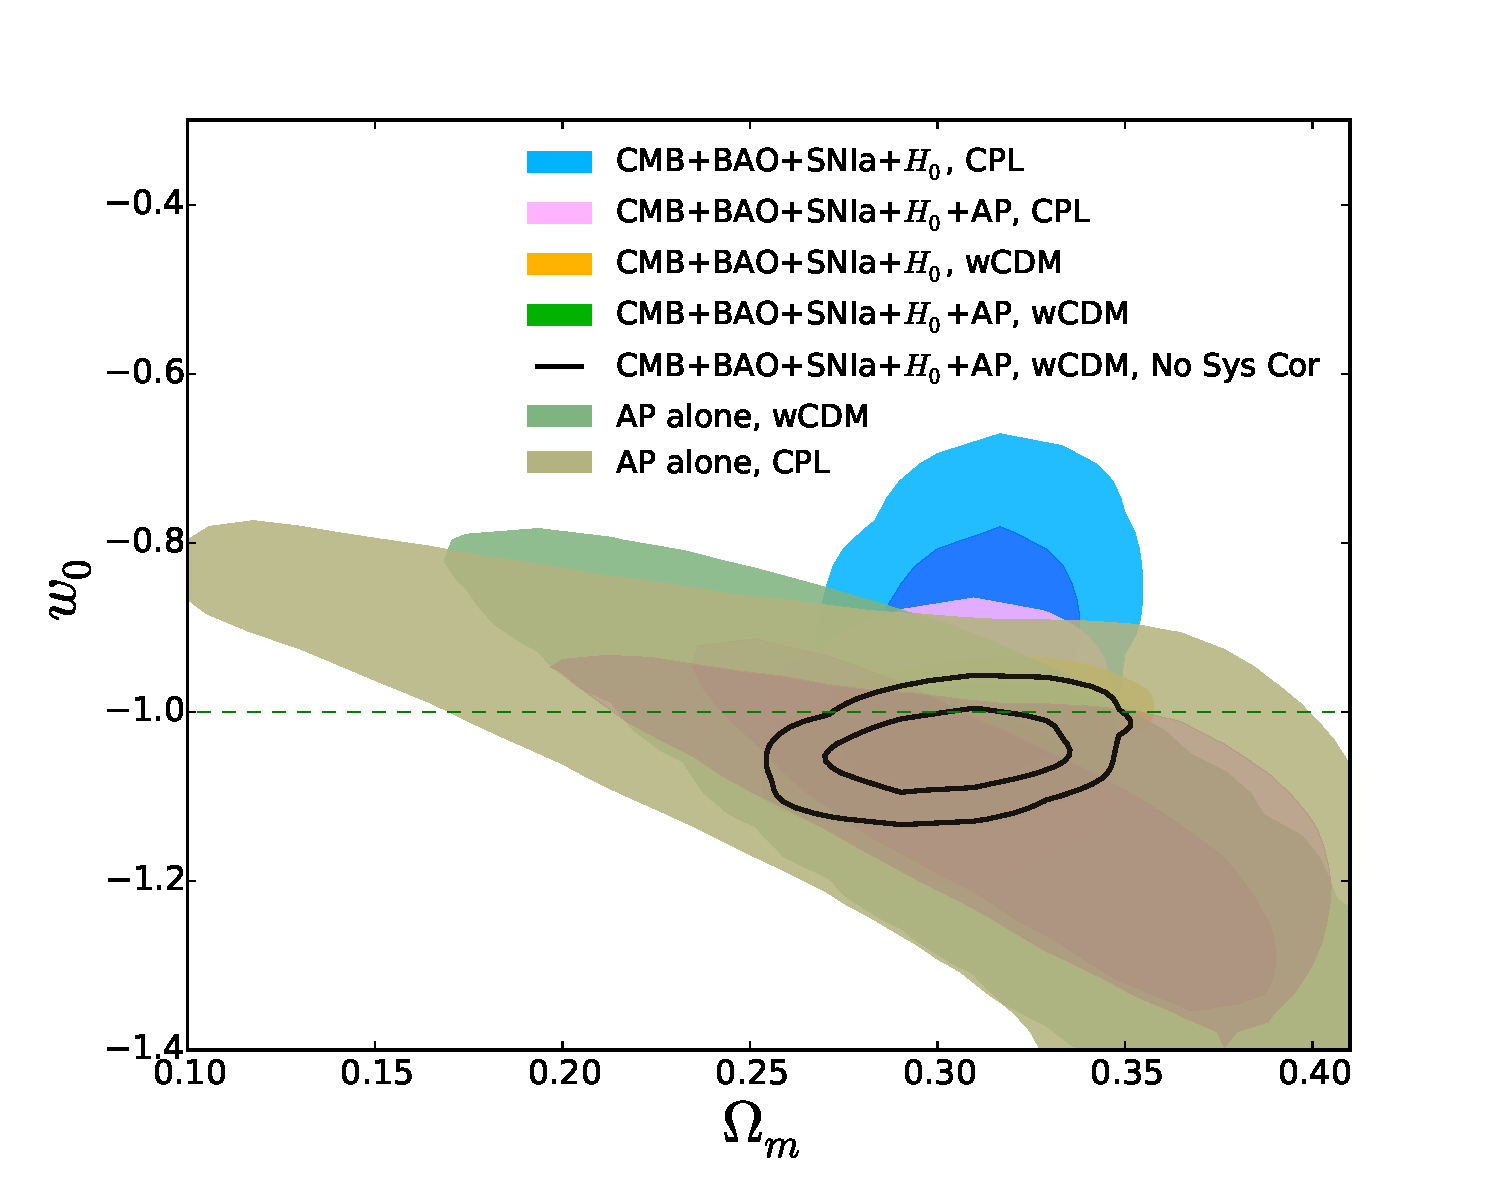
\includegraphics[width=9cm,natwidth=4,natheight=4]{figCPL_a.pdf}
   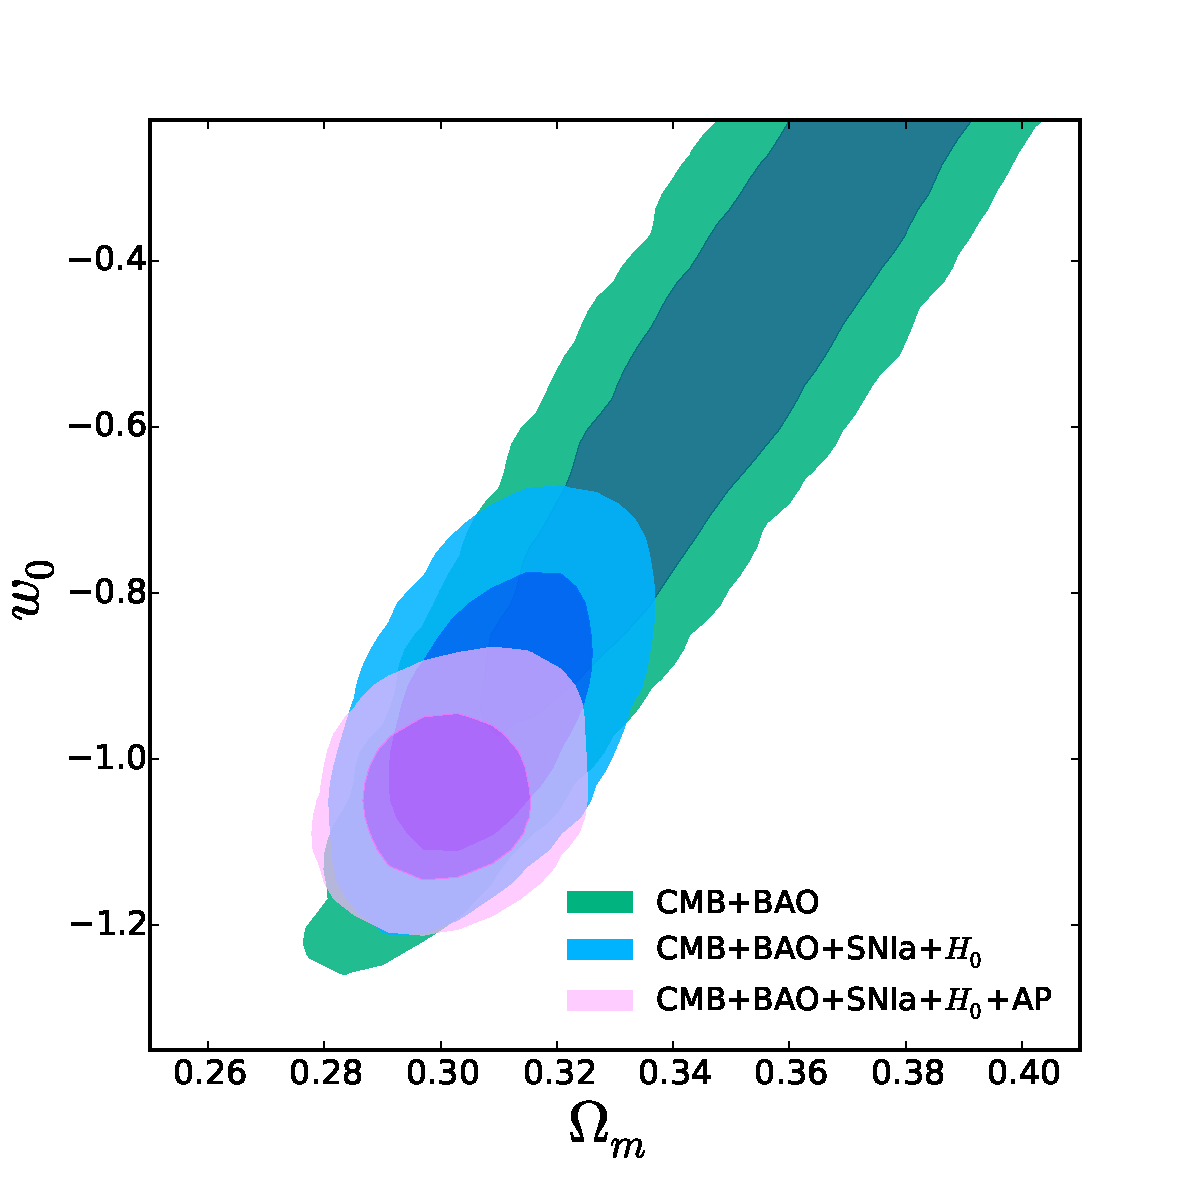
\includegraphics[width=8.3cm,natwidth=8,natheight=8]{figCPL_a1.pdf}
   %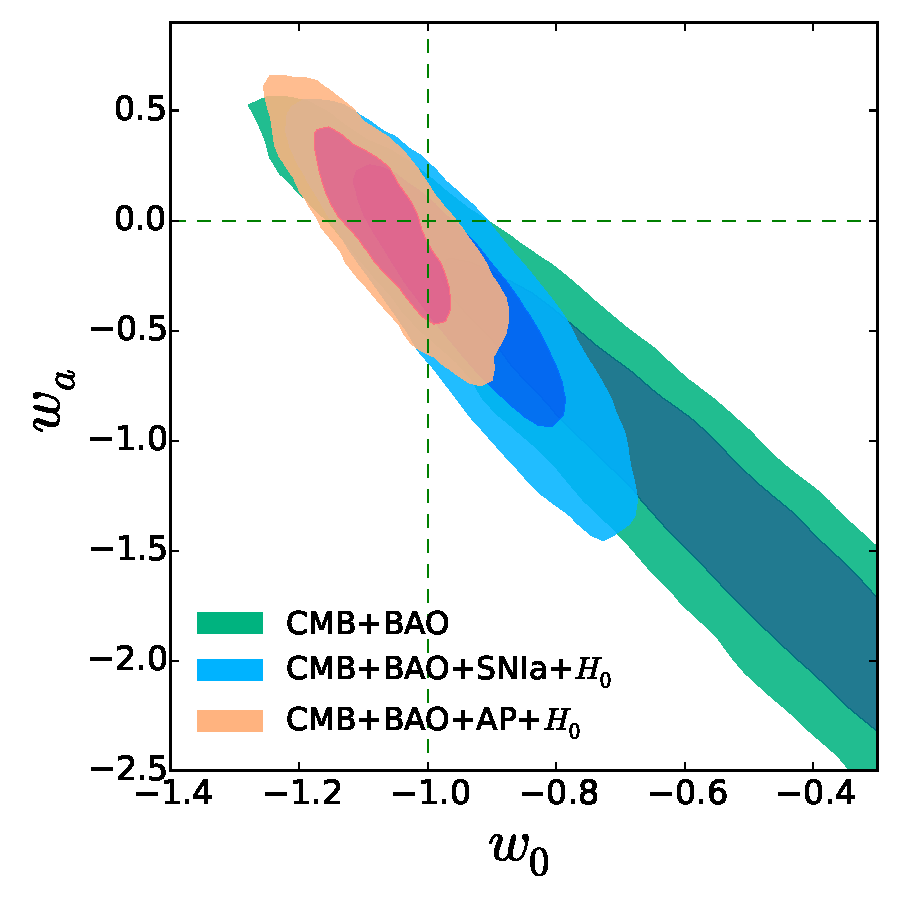
\includegraphics[width=5.5cm,natwidth=4,natheight=4]{figCPL_b_BAOSNIaAP.pdf}
   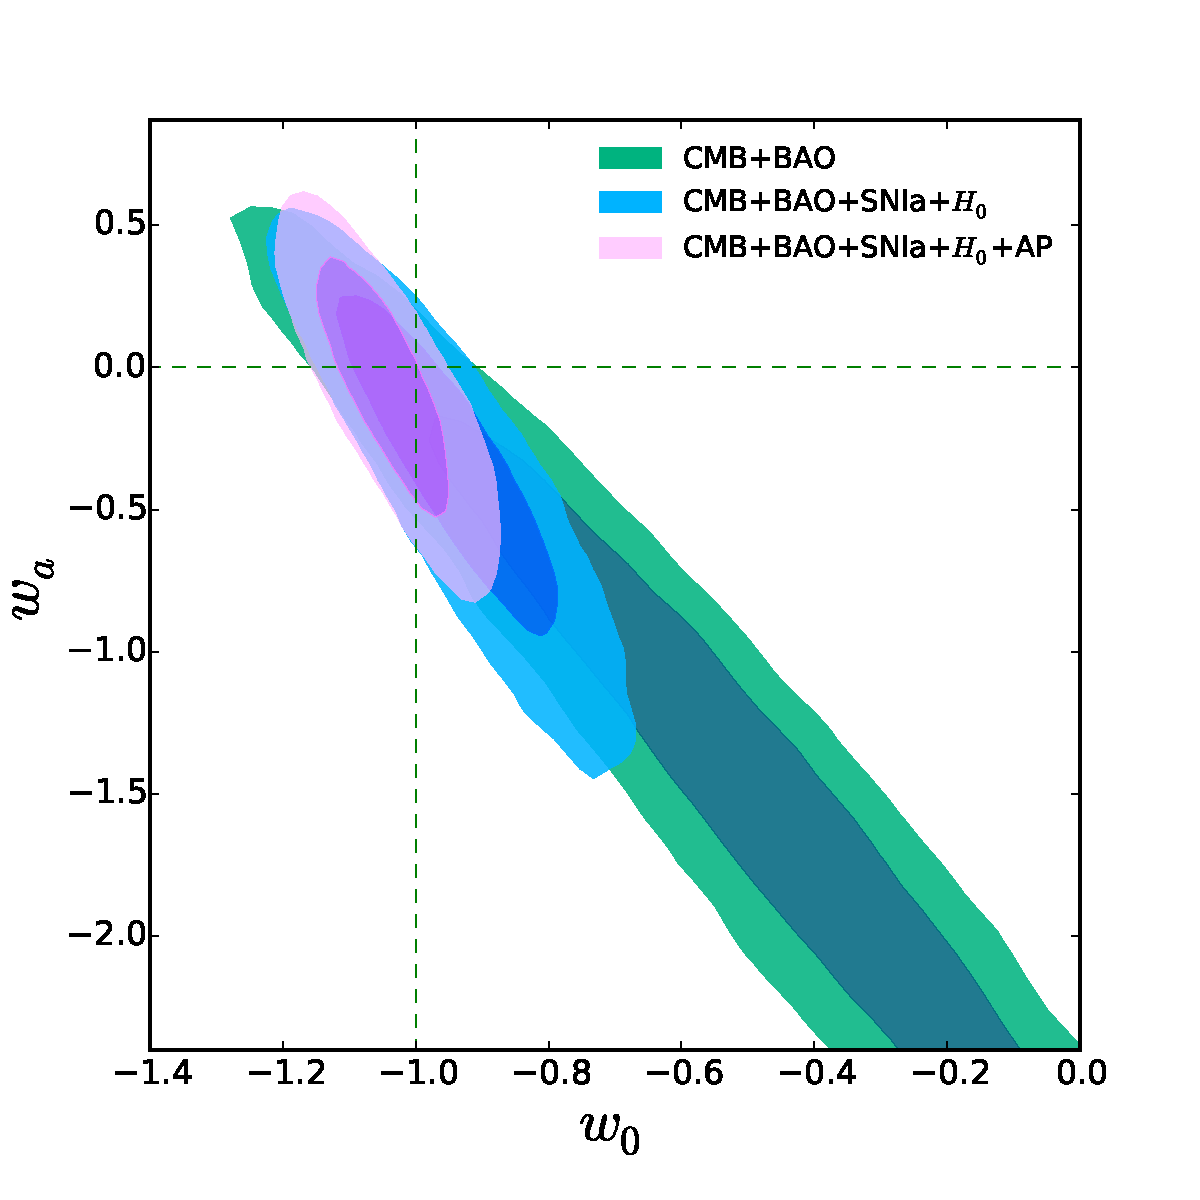
\includegraphics[width=8.3cm,natwidth=8,natheight=8]{figCPL_a2.pdf}
   %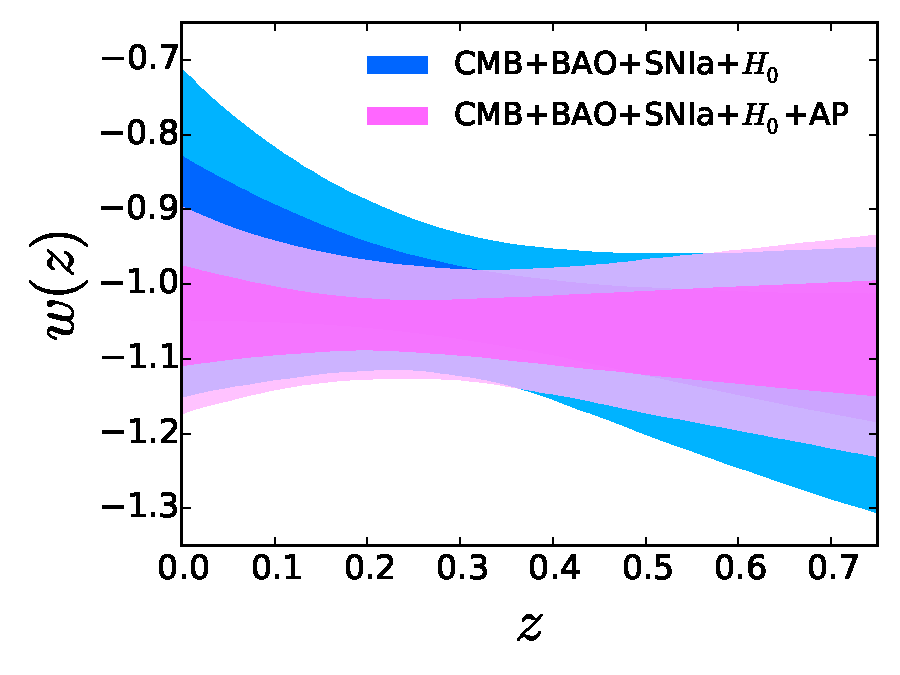
\includegraphics[width=18cm,natwidth=16,natheight=7]{figCPL_d.pdf}
   %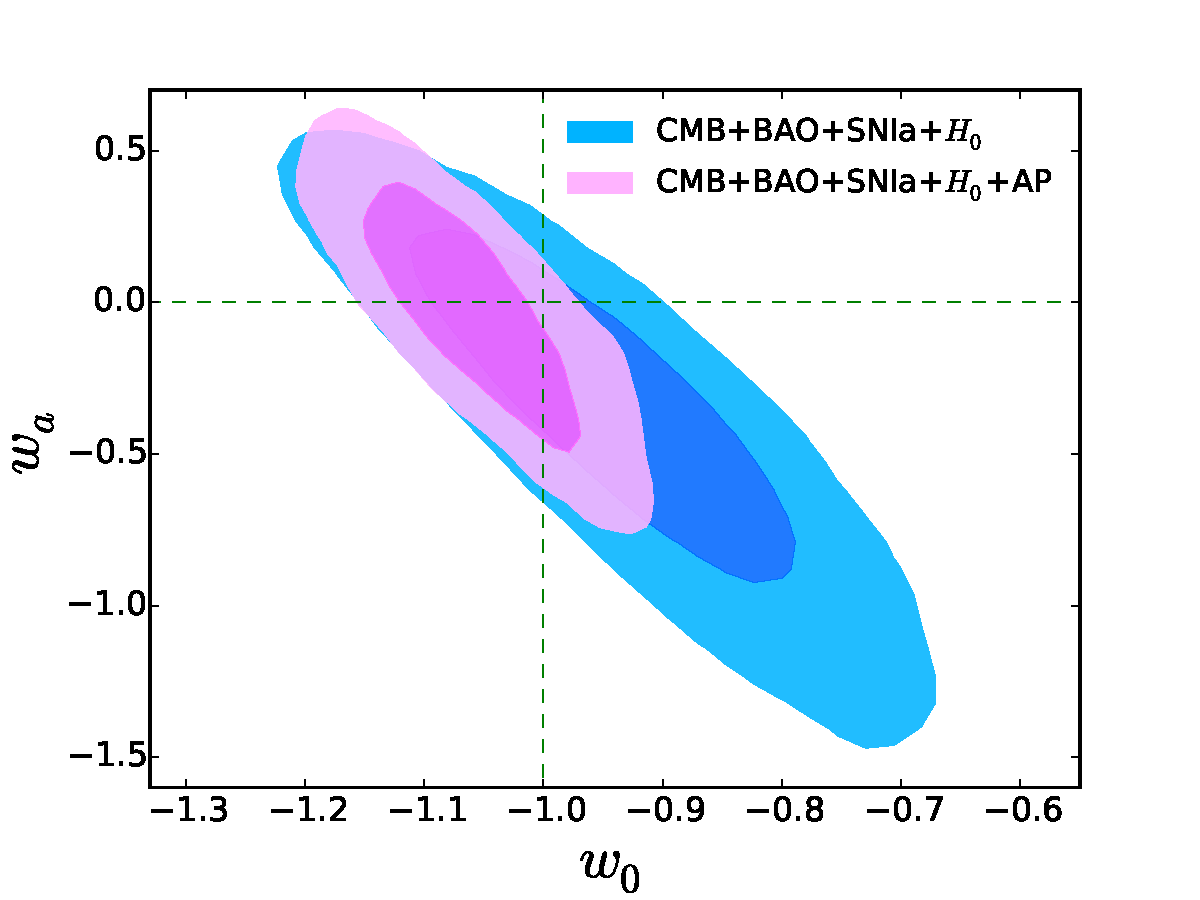
\includegraphics[height=8cm]{fig2b.pdf}
%   \includegraphics[height=8cm]{Tpcf--plot--Normed.eps}
%    \includegraphics[height=8cm]{smu.eps}
   }
   \caption{\label{fig_con}
   Cosmological parameter constraints on the CPL dark energy parametrization $w=w_0+w_a {z}/{(1+z)}$.
   The 68.3\%, 95.4\% CL likelihood contours in the $\Omega_m - w_0$  and $w_0 - w_a$ planes are plotted in the left and right panels, respectively.
   %Results from the AP method alone (brown filled), CMB+BAO (cyan filled), CMB+BAO+SNIa+$H_0$ (blue filled)
   Results from CMB+BAO (cyan filled), CMB+BAO+SNIa+$H_0$ (blue filled)
   and CMB+BAO+SNIa+$H_0$+AP (magenta filled) are shown.
   %To see the effect of systematic effect, we also plot the AP alone and CMB+BAO+SNIa+$H_0$+AP constraints 
   %before conducting the systematics correction procedure (the gray solid and black dashed lines, labeled by ``with sys'').
   %The AP method leads to competitive constraints on the cosmological parameters.
   Adding our AP method to the CMB+BAO+SNIa+$H_0$ combination reduces the contour area by as much as 50\%. %significantly reduced the area of contour.
   %Systematics does not have significant influence on the results.% are less affected by systematics effect.
   %If we discard the systematics correction, there is half-$\sigma$ shift of the AP alone contour.
   %The combined constraints are less affected.
   %This suggests that, for the data analysis of current galaxy surveys,
   %the systematic effects in our method is not significant.
   %This shows the power of the AP method in constraining dynamical dark energy.
   %Middle panel: $w_0-w_a$ likelihood contours using datasets of CMB+BAO, CMB+BAO+SNIa+$H_0$ and CMB+BAO+AP+$H_0$.
   %When combined with CMB+BAO, AP method yields much tighter constraints than SNIa.
   %Right panel: Redshift evolution of $w(z)$, with/without adding the AP constraint.
   %Adding AP tightens the constraints and reduces the redshift evolution of $w$ (tilt of $w(z)$).
   }
\end{figure*}


\begin{figure*}
   \centering{
   %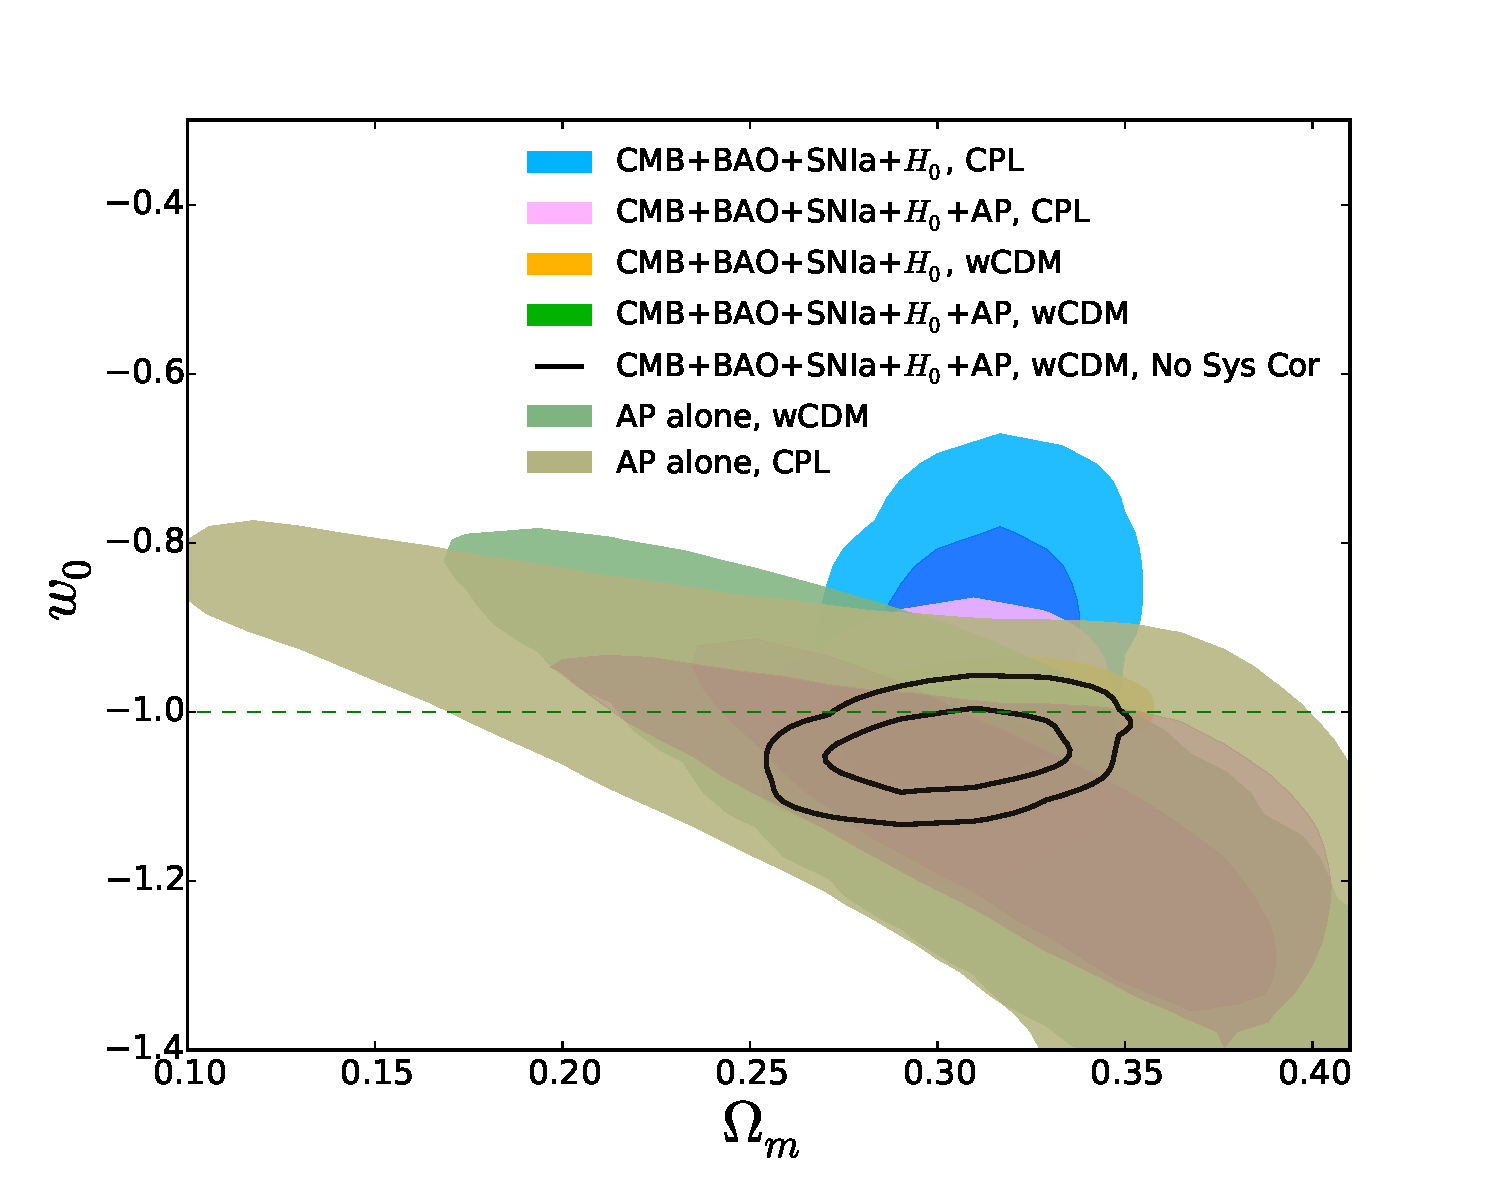
\includegraphics[width=9cm,natwidth=4,natheight=4]{figCPL_a.pdf}
   %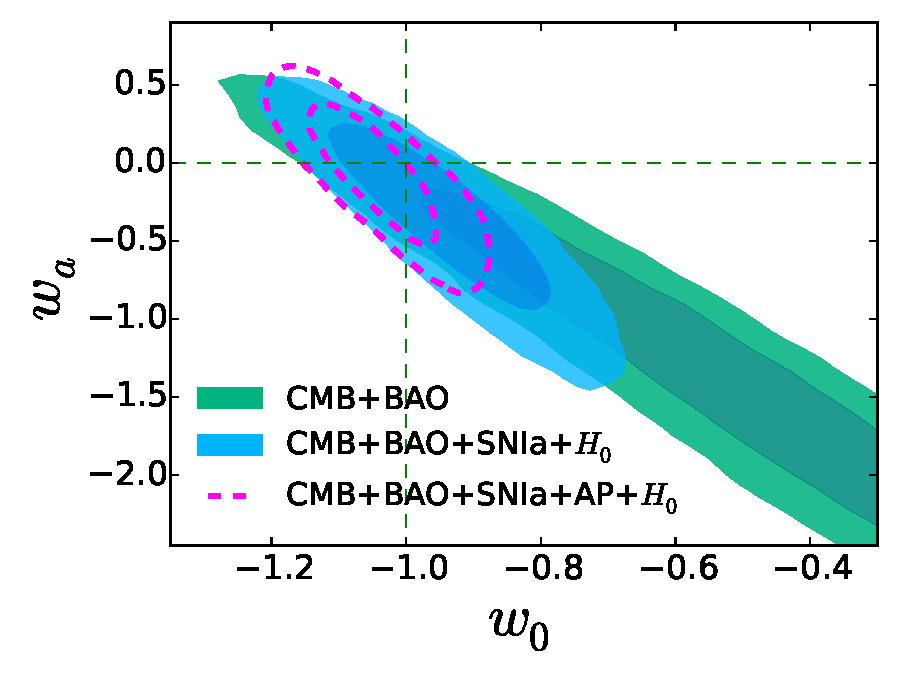
\includegraphics[width=8cm,natwidth=6,natheight=4.5]{figCPL_b.pdf}
   %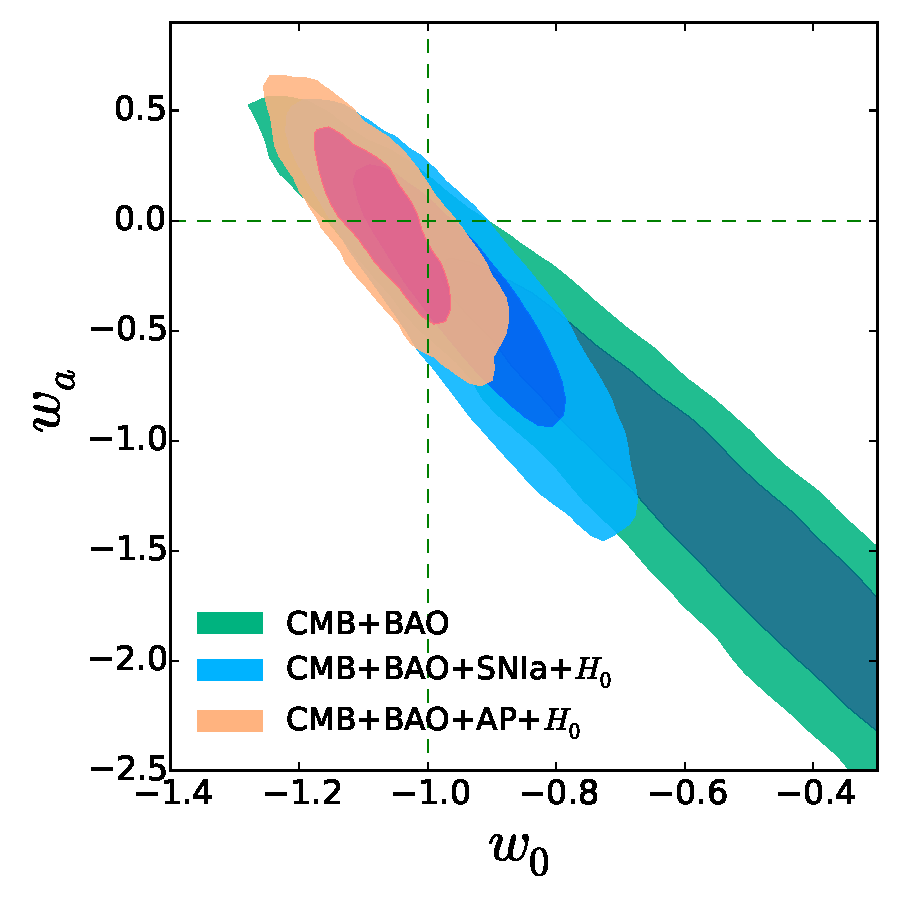
\includegraphics[width=5.5cm,natwidth=4,natheight=4]{figCPL_b_BAOSNIaAP.pdf}
   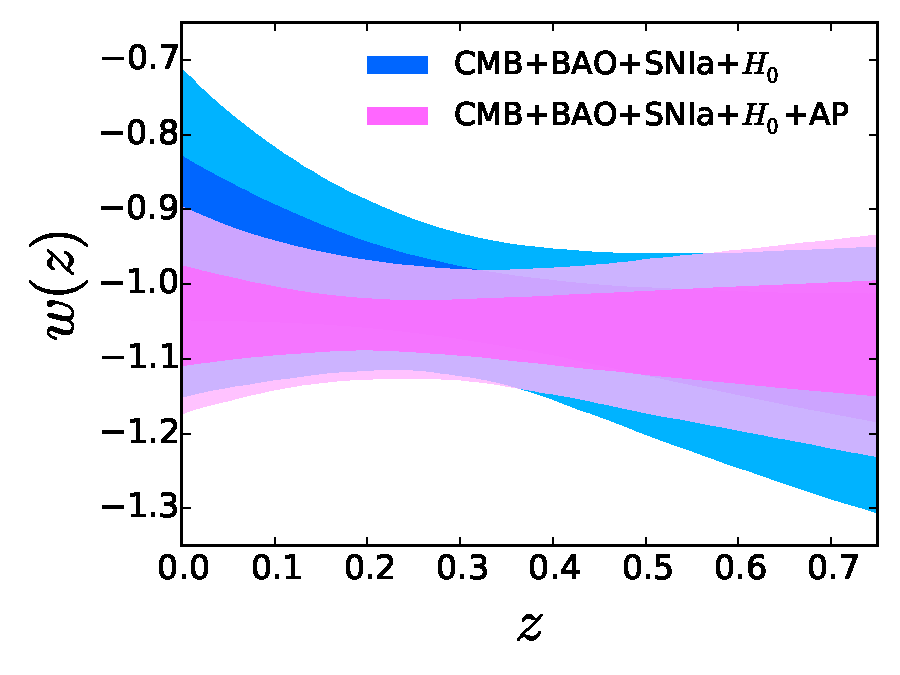
\includegraphics[width=11cm,natwidth=9,natheight=7]{figCPL_d.pdf}
   %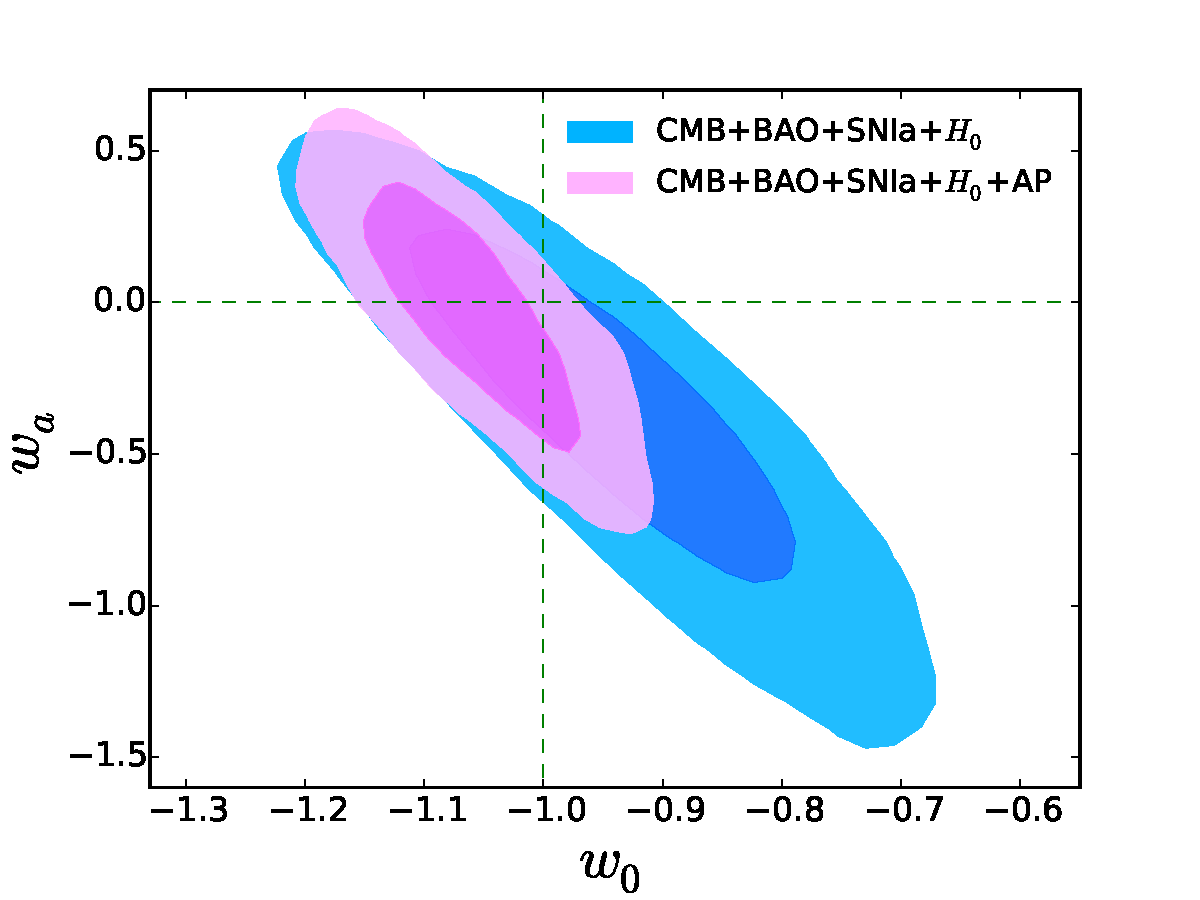
\includegraphics[height=8cm]{fig2b.pdf}
%   \includegraphics[height=8cm]{Tpcf--plot--Normed.eps}
%    \includegraphics[height=8cm]{smu.eps}
   }
   \caption{\label{fig_wz}
   %Cosmological constraints on the CPL dark energy parametrization $w=w_0+w_a\frac{z}{1+z}$.
   %Left panel: 68.3\%, 95.4\% CL likelihood contours in the  $w_0-w_a$ plane.
   %Results are consistent with $\Lambda$CDM.
   %The constrained area is significantly reduced after combined with the AP method.
   %This shows the power of the AP method in constraining dynamical dark energy.
   %Middle panel: $w_0-w_a$ likelihood contours using datasets of CMB+BAO, CMB+BAO+SNIa+$H_0$ and CMB+BAO+AP+$H_0$.
   %When combined with CMB+BAO, AP method yields much tighter constraints than SNIa.
   %Derived redshift evolution of $w(z)$, with/without adding the AP method.
   Derived redshift evolution of $w(z)$, the 68.3\% and 95.4\% CL regions are plotted.
   Adding the AP method tightens the constraints and reduces the redshift evolution of $w$ (the tilt of $w(z)$).
   %There is no significant change in the results if we discard the systematics correction procedure in the AP method analysis.
   }
\end{figure*}



%While the central values of parameters do not shift appreciably,
%Covariance matrix 


Figure \ref{fig_con} shows the 68.3\% and 95.4\% CL likelihood contours in the $\Omega_m - w_0$  and $w_0 - w_a$ planes,
derived from the CMB+BAO, CMB+BAO+SNIa+$H_0$ and CMB+BAO+SNIa+$H_0$+AP, respectively.
The overlapping of different contours suggest that they are consistent with each other.

%Using the AP method alone can lead to effective constraints on the $\Omega_m-w_0$ parameter space.
%Due to the inclusion of one extra free parameter, 
%the constrained area becomes larger than the $w$CDM result.
%Given current galaxy surveys it is difficult to effectively constrain $w_a$ using only one technique.
%We have to combine various techniques.

We can not derive effective constraint on the parameter space from a combination of CMB+BAO.
Combining the four external techniques, i.e. CMB+BAO+SNIa+$H_0$, leads to effective constraints on all parameters.
The statistical mean values and 68.3\% uncertainties of these parameters are
\begin{eqnarray}
&\Omega_m = 0.309 \pm 0.010,\\
&w_0 = -0.938 \pm 0.109,\\
&w_a = -0.38 \pm 0.41,
\end{eqnarray}
while adding our AP method to this combination further tightens the constraints and yield to
\begin{eqnarray}
&\Omega_m = 0.301 \pm 0.008,\\
&w_0 = -1.042 \pm 0.067,\\
&w_a = -0.07 \pm 0.29.
\end{eqnarray}
The error bars are dramatically reduced by 30 -- 40\%,
and the contour areas are reduced by 50\%, i.e., the dark energy figure of merit was improved by 100\%. 
Notice that the AP constraints come from the BOSS DR12 data, which is already used in the BAO analysis.
So the doubling of the figure of merit comes at no additional cost or alteration to data size,
thus greatly improves the overall cost-benefit of the large cosmological redshift surveys.


It can be also noted that, after adding the AP method, the central value of $w_a$ moved significantly towards zero.
This means the result becomes more consistent with a cosmological constant dark energy component having no evolution.
Figure \ref{fig_wz} shows the redshift evolution of $w(z)$ derived from the cosmological constraints.
Adding AP tightens the constraints and reduces the redshift evolution of $w$ (tilt of $w(z)$).


\begin{figure*}
   \centering{
   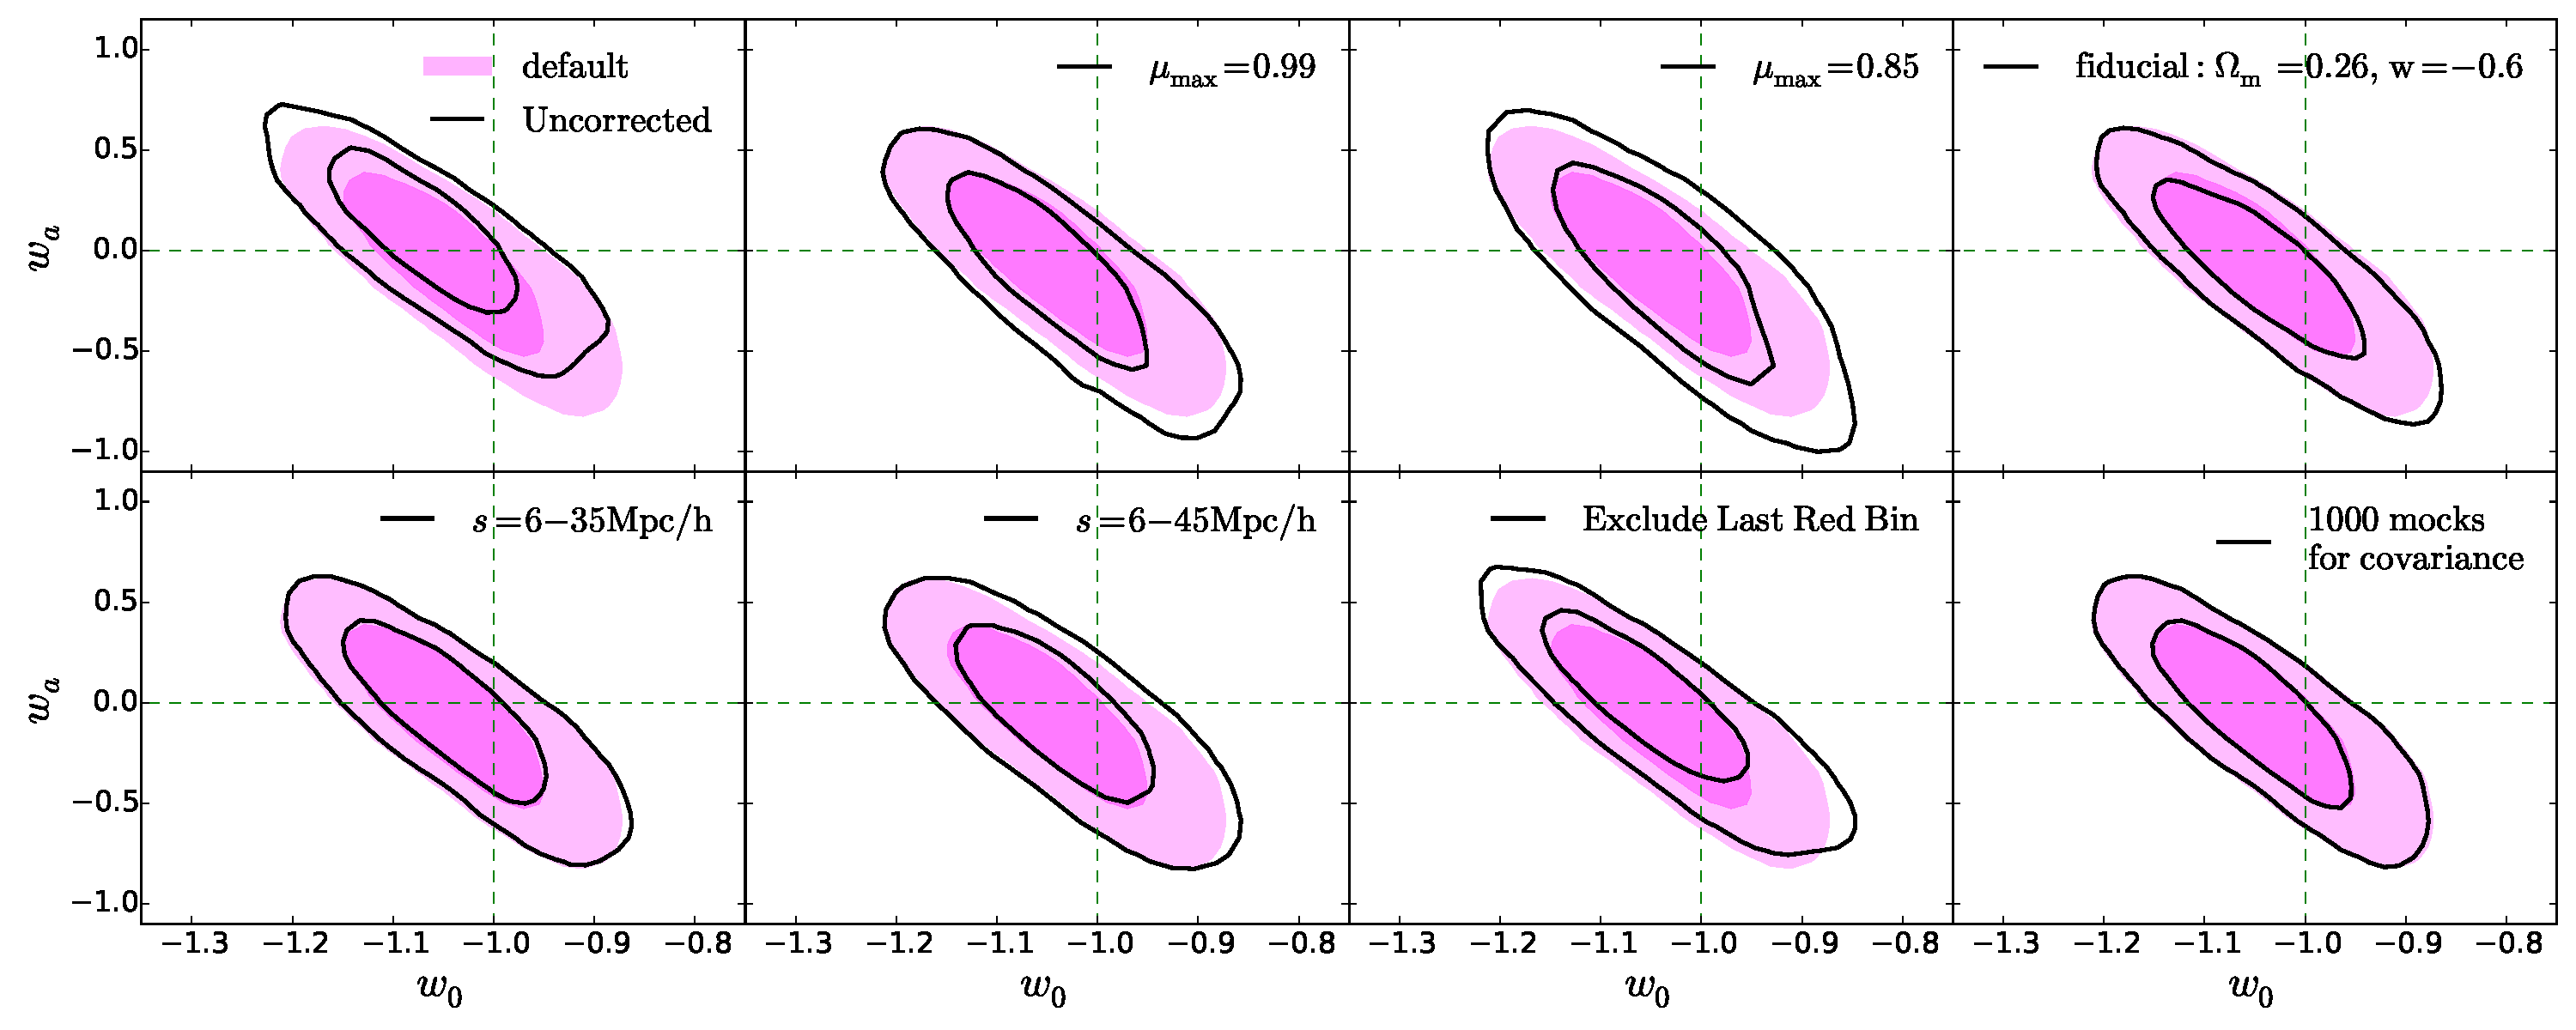
\includegraphics[width=18cm,natwidth=6,natheight=5]{fig_con_tests.pdf}
   %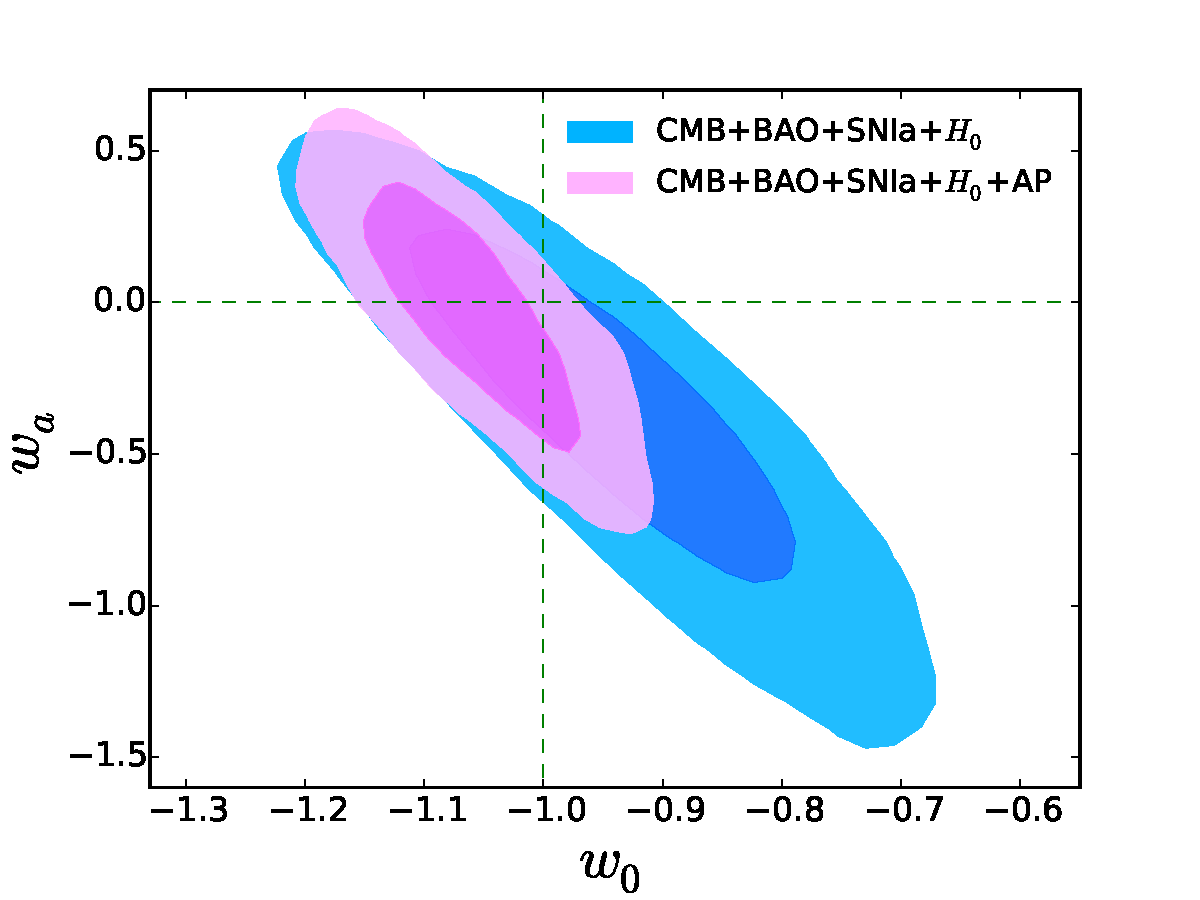
\includegraphics[width=9cm,natwidth=4,natheight=4]{fig2b.pdf}
   %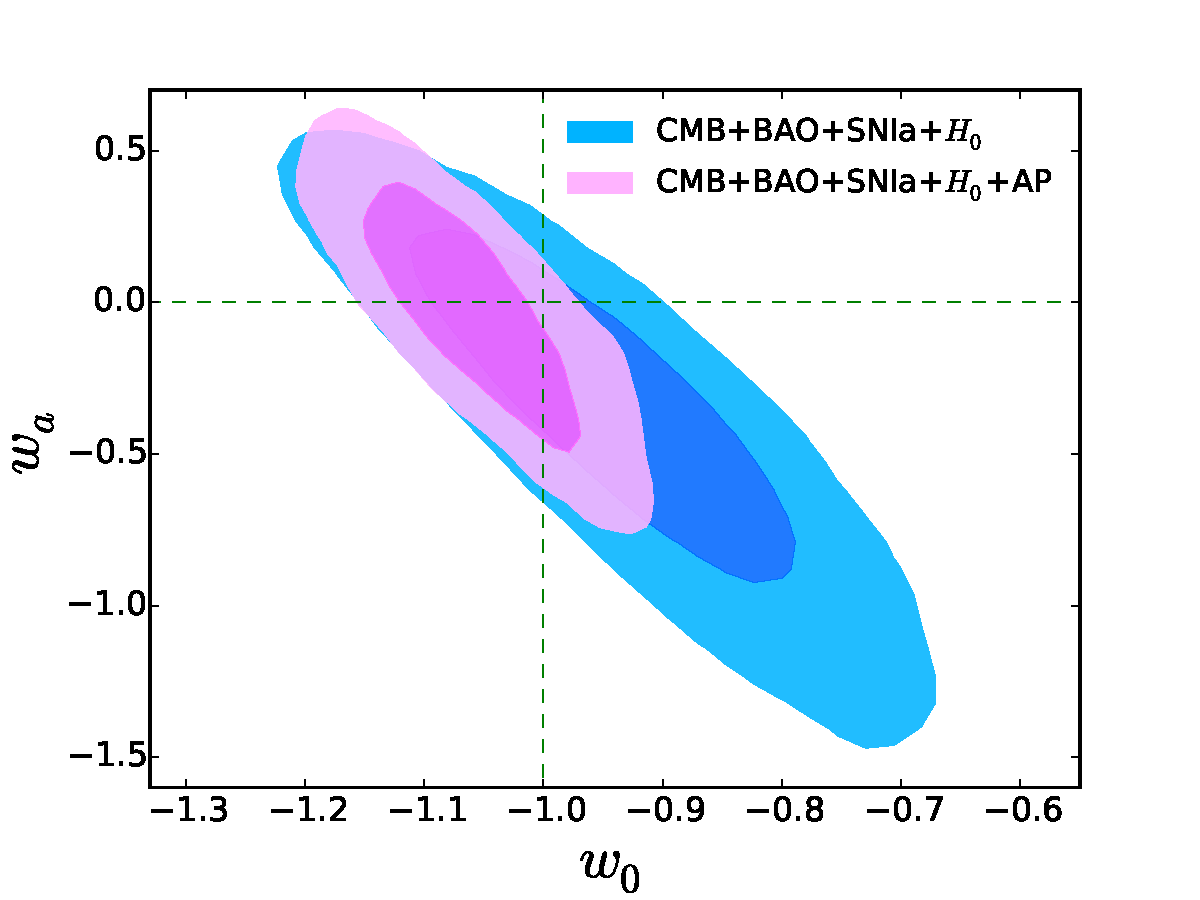
\includegraphics[height=8cm]{fig2b.pdf}
%   \includegraphics[height=8cm]{Tpcf--plot--Normed.eps}
%    \includegraphics[height=8cm]{smu.eps}
   }
   \caption{\label{fig_contest}
   Robustness test of the results.
   The ``default'' constraints (magenta contours) are derived using six redshift bins, 
   $\mu_{\rm max}=0.97$, $s=6 - 40 \rm Mpc/h$,
   a fiducial cosmology $\Omega_m=0.26,\ w=-1.0$ for the approximation of 2PCF,
   systematic effects estimated from Horizon Run 4 simulations, 
   and covariance estimated using 2,000 MultiDark PATCHY mocks.
   When we alters one of these options by discarding the systematic correction, 
   using $\mu_{\rm max}=0.99$, 
   $\mu_{\rm max}=0.85$, $s=6 - 35 \rm Mpc/h$, $s=6 - 45 \rm Mpc/h$,  
   a fiducial cosmology of $\Omega_m=0.26,\ w=-0.6$, 
   excluding the last redshift bin in the analysis, 
   or reducing the number of mocks in the estimation of covariance matrix,
   the results remain robust (black contours).
   }
\end{figure*}

\begin{figure*}
   \centering{
   %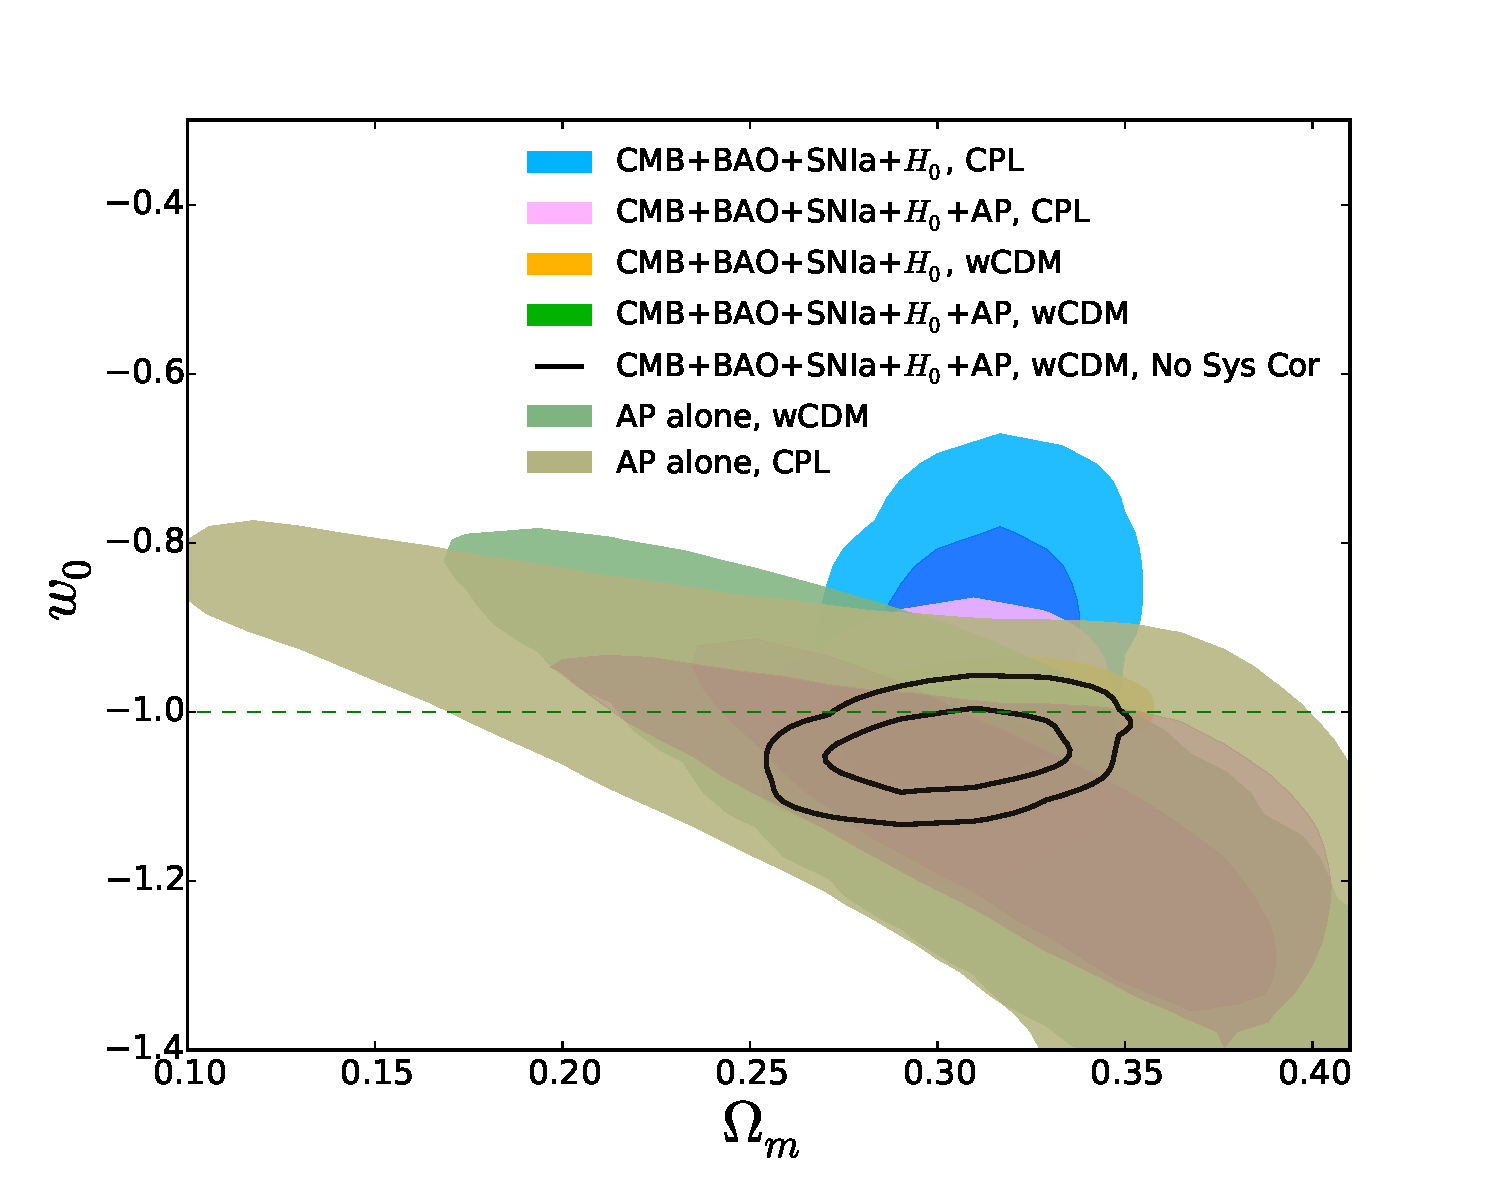
\includegraphics[width=9cm,natwidth=4,natheight=4]{figCPL_a.pdf}
   %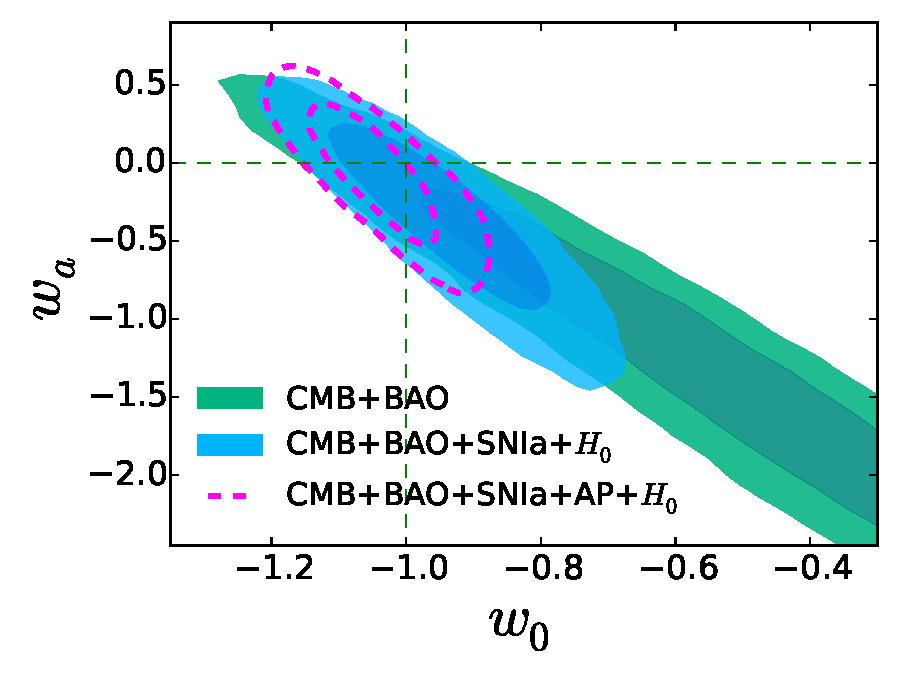
\includegraphics[width=8cm,natwidth=6,natheight=4.5]{figCPL_b.pdf}
   %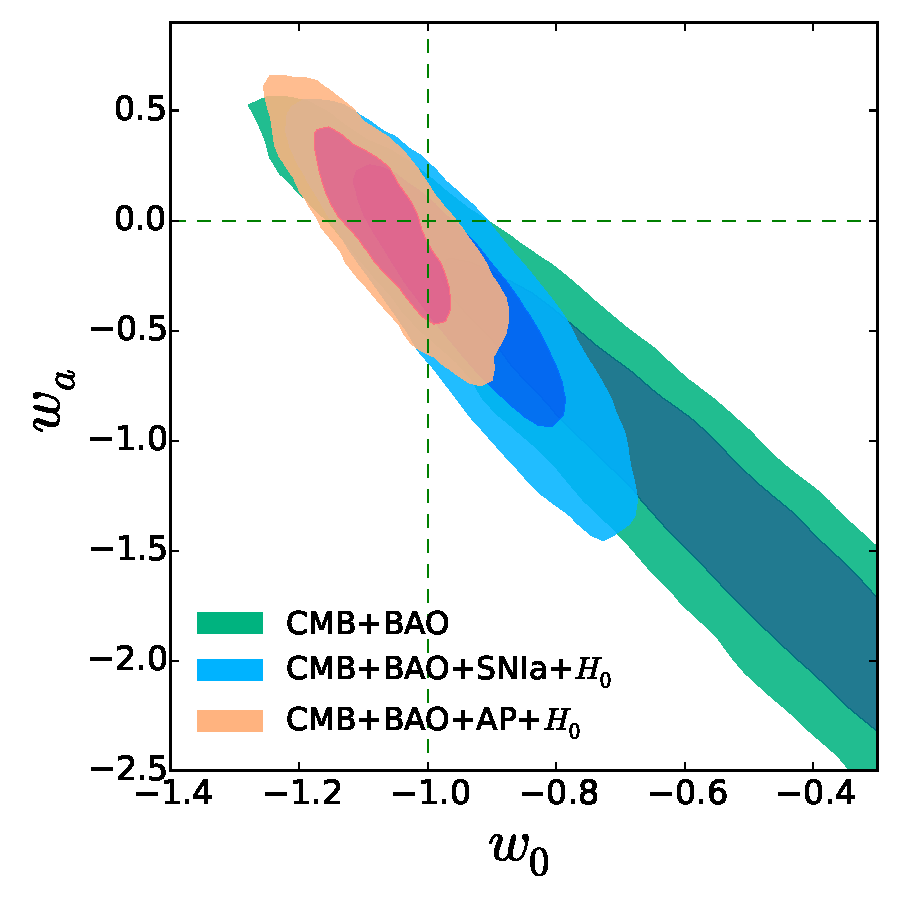
\includegraphics[width=5.5cm,natwidth=4,natheight=4]{figCPL_b_BAOSNIaAP.pdf}
   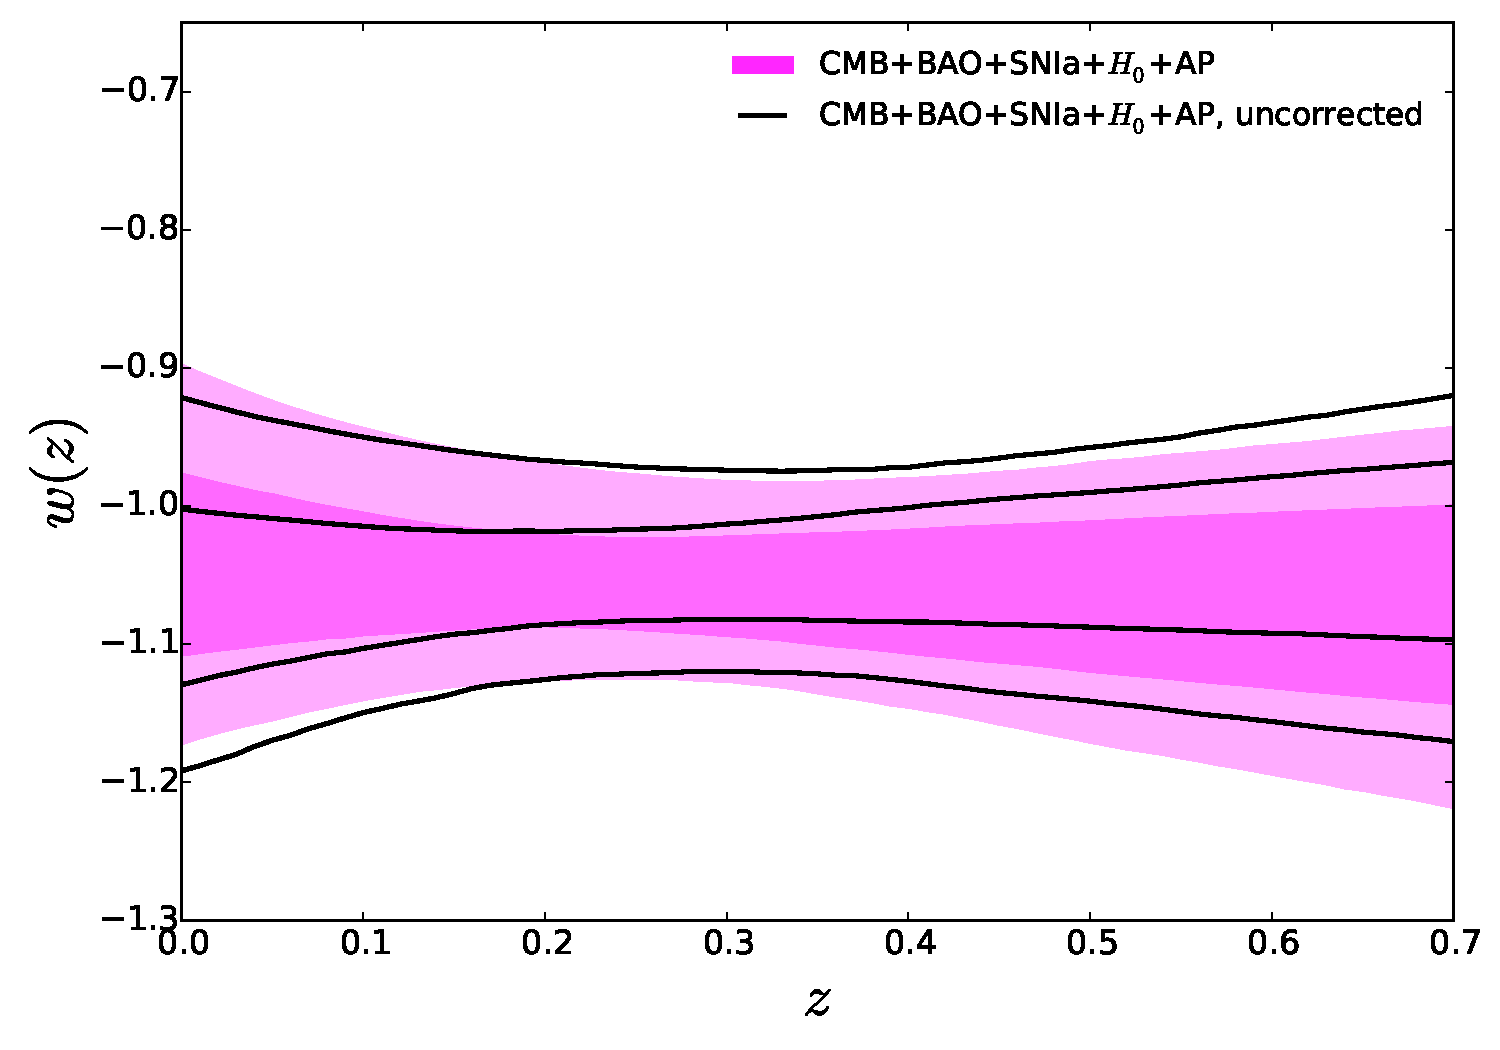
\includegraphics[width=11cm,natwidth=9,natheight=7]{figCPL_d_withsys.pdf}
   %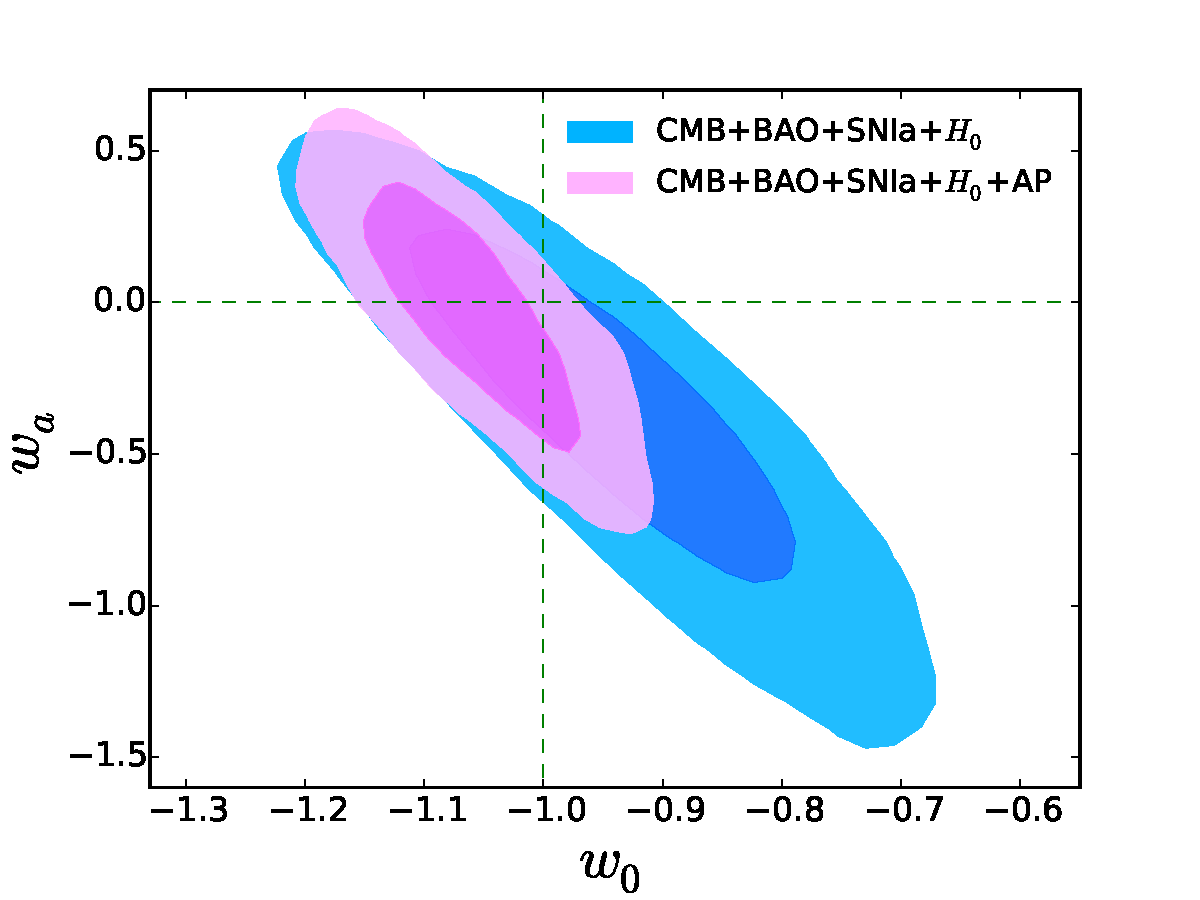
\includegraphics[height=8cm]{fig2b.pdf}
%   \includegraphics[height=8cm]{Tpcf--plot--Normed.eps}
%    \includegraphics[height=8cm]{smu.eps}
   }
   \caption{\label{fig_wz_sys}
   %Cosmological constraints on the CPL dark energy parametrization $w=w_0+w_a\frac{z}{1+z}$.
   %Left panel: 68.3\%, 95.4\% CL likelihood contours in the  $w_0-w_a$ plane.
   %Results are consistent with $\Lambda$CDM.
   %The constrained area is significantly reduced after combined with the AP method.
   %This shows the power of the AP method in constraining dynamical dark energy.
   %Middle panel: $w_0-w_a$ likelihood contours using datasets of CMB+BAO, CMB+BAO+SNIa+$H_0$ and CMB+BAO+AP+$H_0$.
   %When combined with CMB+BAO, AP method yields much tighter constraints than SNIa.
   %Derived redshift evolution of $w(z)$, with/without adding the AP method.
   Derived redshift evolution of $w(z)$ from CMB+BAO+SNIa+$H_0$+AP.
   %Adding the AP method tightens the constraints and reduces the redshift evolution of $w$ (the tilt of $w(z)$).
   There is no significant change if we discard the systematics correction procedure in the AP method analysis.
   }
\end{figure*}

\subsection{Robustness}

%The effect of our systematic correction can be seen in Figures \ref{fig_con} and \ref{fig_wz} 
%where we plot the AP alone and CMB+BAO+SNIa+$H_0$+AP combined constraints 
%before conducting the systematics correction procedure.
Figure \ref{fig_contest} and \ref{fig_wz_sys} show that,
if we discard the systematics correction, %there is a half-$\sigma$ shift of the AP alone constraints;
%since the direction of shift is orthogonal to the direction of CMB+BAO+SNIa+$H_0$ contour,
the derived constraints are almost unaffected.
This indicates that, for the data analysis of current galaxy surveys,
the systematic effects in our method is not significant. 
But it remains to be seen if this is true for future galaxy surveys,
or when the cosmology dependence of the systematics effects is taken into account.
%The results are less affected by systematics.
%\cite{Li2016} 


%Finally, we performed a test of all the possible variables in our methodology.
Furthermore, Figure \ref{fig_contest} shows that 
the result is unaffected by the line-of-sight $\mu$-cut, 
the range of radial integration, 
the choice of fiducial cosmology in the mapping of $\xi(s,\mu)$,
and the number of mocks.
%Reduces the number of angular bins weakens the constraints a little bit,
%and enlarges the contour towards the lower-right direction 
%(the upper-left boundary is determined by the CMB+BAO+SNIa+$H_0$ constraints, so it is unaffected).
%we adopt $\mu_{\rm max}=0.99\ (0.85)$ to include more (less) regions near the LOS,
%decrease the number of angular bins to $n_{\mu}=15-20$,
%change the range of clustering to $8-30 \rm Mpc/h$,
%change the fiducial cosmology to $\Omega_m=0.26,\ w=-0.6$,
%exclude 1 or 2 high redshift bins,
%or reduce the number of mocks to 1000.
The result does not change significantly if we remove the highest redshift bin,
where the estimated systematics is comparably large.
This further justifies our conclusion that, the effect of systematics is not significant in this analysis.


%\section{Conclusion}\label{sec:conclusion}
\section{Conclusion}

In recent studies we have proposed to constrain cosmological parameters 
governing the expansion history of the universe via 
the redshift dependence of anisotropic galaxy clustering \citep{Li2014,Li2015,Li2016}.
This approach enables a robust AP test on relatively small scales.
In this paper we improved the methodology and obtained a tight constraint 
on the CPL parametrization of dark energy.
The derived cosmological constraints are fully consistent with a cosmological constant 
dark energy component having no redshift evolution.

%using 1,133,326 galaxies from the Sloan Digital Sky Survey Data Release 
%12 spanning the redshift range $0.15<z<0.69$ . 
%Adding our constraints to the CMB+SNIa+BAO+$H_0$ combination, the $w_0-w_a$ contour was reduced by $\sim50$\%.

The AP method presented in this work has many advantages over the 
`traditional' methods using galaxy clustering.
Since it works with the redshift evolution of the anisotropic clustering signal it significantly reduces the effect of systematics. 
It avoids the great difficulty in accurate modeling of the RSD, non-linear clustering and galaxy bias.
%It is applicable on much smaller clustering scales, allowing for the inclusion of more $k$-modes and hence more information. 
Our method can use the galaxy clustering signal down to
much smaller scales compared to other methods,
providing much higher statistics.


%Yet there are still issues demanding more investigations.
In this analysis, we find that the systematic effects do not significantly affect the derived cosmological constraints.
But it remains to be seen if this is true for future galaxy surveys.
Especially, the systematic effects are estimated using simulations performed in a certain cosmology.
The cosmological dependence remains to be investigated in future works.


In this analysis, combining our method with the CMB+SNIa+BAO+$H_0$ datasets,
the dark energy figure of merit is improved by a factor of 2.
%The method can be applied to many spectroscopic galaxy surveys.
This indicates the great power of the method in constraining the cosmic expansion history and probing the properties of dark energy.
We expect the method will play an important role in deriving cosmological constraints from future spectroscopic galaxy surveys.



\section*{Acknowledgments}

We thank Korea Institute for Advanced Study for providing computing resources (KIAS Center for Advanced Computation Linux Cluster System).
CGS acknowledges support from the National Research Foundation (NRF,  \#2017R1D1A1B03034900). 
We thank Stephen Appleby, Seokcheon Lee, Maurice van Putten, Graziano Rossi and Yi Wang for helpful discussions.

Based on observations obtained with Planck (http://www.esa.int/Planck), 
an ESA science mission with instruments and contributions directly funded by 
ESA Member States, NASA, and Canada.


Funding for SDSS-III has been provided by the Alfred P. Sloan Foundation, the Participating Institutions, the
National Science Foundation, and the U.S. Department of Energy Office of Science. 
The SDSS-III web site is http://www.sdss3.org/. 
SDSS-III is managed by the Astrophysical Research Consortium for the Participating Institutions
of the SDSS-III Collaboration including the University of Arizona, the Brazilian Participation Group, Brookhaven
National Laboratory, Carnegie Mellon University, University of Florida, the French Participation Group, 
the German Participation Group, Harvard University, the Instituto de Astrofisica de Canarias, the Michigan State/Notre
Dame/JINA Participation Group, Johns Hopkins University, Lawrence Berkeley National Laboratory, Max Planck
Institute for Astrophysics, Max Planck Institute for Extraterrestrial Physics, New Mexico State University, New
York University, Ohio State University, Pennsylvania State
University, University of Portsmouth, Princeton University,
the Spanish Participation Group, University of Tokyo, University of Utah, Vanderbilt University, University of Virginia, 
University of Washington, and Yale University.

\

\

\

\begin{thebibliography}{}

\bibitem[Ade et al. (2015)]{Planck2015}
Ade, P.A.R., Aghanim, N., \& Arnaud, M., et al. arXiv:1502.01589

\bibitem[Alam et al.(2016)]{Alam2016}
Alam, S., Ata, M., \& Bailey, S., et al. 2016,
submitted to MNRAS (arXiv:1607.03155)

\bibitem[Albrecht et al.(2006)]{DETF}
Albrecht, A., Bernstein, G., \& Cahn, R., et al. 2006. [astro-ph/0609591].


%\bibitem[{{Alam} {et~al}\mbox{.}(2015{\natexlab{a}}){Alam}, {Albareti},
%  {Allende Prieto}, {Anders}, {Anderson}, {Anderton}, {Andrews}, {Armengaud},
%  {Aubourg}, {Bailey}, \& et~al.}]{dr12}
%{Alam} S., Albareti, F.D.,\& Allende Prieto, C., {et~al.}, 2015,  ApJS, 219, 12

\bibitem[Alcock \& Paczynski(1979)]{AP1979}
Alcock, C., \& Paczynski, B. 1979, Nature, 281, 358  

%\bibitem[Anderson et al.(2012)]{2012MNRAS.427.3435A} 
%Anderson, L., Aubourg, E., Bailey, S., et al.\ 2012, MNRAS, 427, 3435

\bibitem[Anderson et al.(2013)]{Anderson2013}
Anderson, L., Aubourg, \'E., \& Bailey, S. et al. 2014, MNRAS, 441, 24  
  
%\bibitem[Bassett et al.(2002)]{Bassett2002}
%Bassett, B.A., Kunz, M., Silk, J., \& Ungarelli, C. 2002, MNRAS, 336, 1217

\bibitem[Ballinger, Peacock \& Heavens 1996]{Ballinger1996}
Ballinger, W.E., Peacock, J.A., \& Heavens, A.F. 1996, MNRAS, 282, 877  

\bibitem[Betoule et al.(2014)]{JLA}
Betoule, M., Kessler, R., \& Guy, J., et al. 2014, A\&A, 568, 32


\bibitem[Beutler et al.(2011)]{6dFGS}
Beutler, F., Blake, C., \& Colless, M., et al. 2011, MNRAS, 416, 3017

%\bibitem[Beutler et al.(2013)]{Beutler2013}
%Beutler, F., Saito, S., \& Seo, H.-J., et al. 2013, MNRAS, 443, 1065

%\bibitem[Beutler et al.(2016)]{Beutler2016}
%Beutler, F., Seo, H.-J., \& Saito, S., et al. 2016,
%arXiv:1607.03150

\bibitem[Blake et al.(2011)]{Blake2011}
Blake, C., Glazebrook, K., \& Davis, T. M., 2011, MNRAS, 418, 1725  

%\bibitem[Blake et al.(2013)]{WiggleZtopoloy}
%Blake, C., James, J.B., \& Poole, G.B. 2013, MNRAS, 437, 2488

%\bibitem[Bolton et al.(2012)]{Bolton2012}
%Bolton, A.S., Schlegel, \& D.J., Aubourg E., et al. 2012, AJ, 144, 144

%\bibitem[Boylan-Kolchin et al.(2008)]{B08}
%Boylan-Kolchin, M., Ma, C.-P., \& Quataert, E. 2008, MNRAS, 383, 93


%\bibitem[Bueno Belloso et al. (2012)]{BB2012}
%Bueno Belloso, A., Pettinari, G.W., Meures, N., \& Percival, W.J. 2012, Phys. Rev. D, 86, 023530

\bibitem[Chevallier \& Polarski(2001)]{CPL_CP}
Chevallier, M., Polarski, D. 2001, Int. J. Mod. Phys. D, 10, 213

%\bibitem{CPL_CP}
%Chevallier, M, \& Polarski, D. 2001, Int. J. Mod. Phys. D,  10, 213


%\bibitem[Choi et al.(2010)]{choi 2010}
%Choi, Y.-Y., Park, C., Kim, J., Gott, J.R., 
%Weinberg, D.H., Vogeley, M.S., \& Kim, S.S. 2010, ApJS, 190, 181

%\bibitem[Christensen et al.(2001)]{Bayesian}
%Christensen, N., Meyer, R., Knox, L., \& Luey, B. 2001, Class. Quant. Grav., 18, 2677

%\bibitem[Chuang et al.(2013)]{Chuang2013}
%Chuang, C.-H., Prada, F., Beutler, F., et al. 2013, arXiv:1312.4889  

%\bibitem[Chuang \& Wang(2012)]{ChuangWang2012}
%Chuang, C.-H., \& Wang, Y. 2012, MNRAS, 426, 226  


%\bibitem[Corasaniti \& Copeland(2003)]{Corasaniti2003}
%Corasaniti, P.S., Copeland, E.J. 2003, Phys. Rev. D, 67, 063521

%eBOSS: 
%http://arxiv.org/abs/1508.04473
%\bibitem[Dawson et al.(2015)]{eBOSS}
%Dawson, K.S., Kneib, J.P., \& Percival, W.J., et al. 2015, accepted AJ

%\bibitem[Dawson et al.(2012)]{Dawson et al. 2012}
%Dawson, K.S., Schlegel, D.J., \& Ahn, C.P., et al. 2012, AJ, 145, 10

\bibitem[Efstathiou (2014)]{E14H0}
Efstathiou, G. 2014, MNRAS, 440, 1138

%\bibitem[Eisenstein et al.(2011)]{Eisenstein et al. 2011}
%Eisenstein, D.J.,  Weinberg, D.H., \& Agolet, E., et al. 2011, AJ, 142, 72

%\bibitem[Feldman, Kaiser \& Peacock (1994)]{1994ApJ...426...23F} 
%Feldman, H.A., Kaiser, N., \& Peacock, J.A.\ 1994, ApJ, 426, 23 

%\bibitem[Fukugita et al. (1996)]{Fukugita1996}
%Fukugita, M., Ichikawa, T., \& Gunn, J.E., et al. 1996, AJ, 111, 1748
%Publication:	
%Astronomical Journal v.111, p.1748 

%\bibitem[Gingold \& Monaghan(1977)]{GM1977}
%Gingold, R.A., \& Monaghan, J.J. 1977, MNRAS, 181, 375  

%\bibitem[Gott et al.(2009)]{gott 2009}
%Gott, J.R., Choi, Y.-Y., Park, C., \& Kim, J. 2009, ApJ, 695, L45  

%\bibitem[Gott et al.(2008)]{gott 2008}
%Gott, J.R., Hambrick, D.C., Vogeley, M.S., Kim, J., Park, C., Choi, Y.-Y.,
%Cen, R., Ostriker, J.P., \& Nagamine, K. 2008, ApJ, 675, 16  


%\bibitem[Gunn et al. (1998)]{Gunn1998}	
%Gunn, J.E., Carr, M., \& Rockosi, C. et al. 1998, AJ, 116, 3040

%\bibitem[Gunn et al.(2006)]{Gunn et al. 2006}
%Gunn, J.E., Siegmund, W.A., \& Mannery, E.J., et al. 2006, AJ, 131, 2332

%\bibitem[Guzzo et al.(2008)]{Guzzo2008}
%Guzzo, L., Pierleoni, M., \& Meneux, B., et al. 2008, Nature, 451, 541

\bibitem[Hartlap et al.(2006)]{Hartlap}
Hartlap J., Simon P. \& Schneider P. [astro-ph/0608064].


\bibitem[Hong et al.(2016)]{hong2016}
Hong, S.E., Park, C.,\&  Kim, J. 2016, ApJ, 823, 103

\bibitem[Jackson (1972)]{FOG}
Jackson, J., 1972, MNRAS, 156, 1

\bibitem[Jennings et al.(2011)]{Jennings2011}
Jennings, E., Baugh, C.M., \& Pascoli, S. 2011, MNRAS, 420, 1079  

%\bibitem[Jeong et al.(2014)]{Jeong2014}
%Jeong, D., Dai, L., Kamionkowski, M., \& Szalay, A.S. 2014, arXiv:1408.4648

%\bibitem[Jiang et al.(2008)]{jiang2008}
%Jiang, C.Y., Jing, Y. P., \& Faltenbacher, A., et al. 2008, ApJ, 675, 1095

\bibitem[Kaiser (1987)]{Kaiser1987}
Kaiser, N. 1987, MNRAS, 227, 1


%\bibitem[Kim \& Park(2006)]{kim and park 2006}
%Kim, J., \& Park, C. 2006, ApJ, 639, 600  

%\bibitem[Kim et al.(2009)]{2009ApJ...701.1547K} 
%Kim, J., Park, C., Gott, J.R., III, \& Dubinski, J.\ 2009, ApJ, 701, 1547 

\bibitem[Kim et al.(2015)]{HR4}
Kim, J., Park, C., L'Huillier, B., \& Hong, S. E. 2015, JKAS, 48, 213

%\bibitem[Kim et al.(2011)]{horizonrun}
%Kim, J., Park, C., Rossi, G., Lee, S.M., \& Gott, J.R. 2011, JKAS, 44, 217  

\bibitem[Kitaura et al.(2015)]{MDPATCHY}
Kitaura, F.S., Rodrı\'{i}guez-Torres, S., Chuang, C.-H., et al. arXiv:1509.06400

\bibitem[Klypin et al.(2016)]{K2014}
Klypin, A., Yepes, G., Gottlober, S., Prada, F., \& Hess, S. 2016,
MNRAS, 457, 4340%

\bibitem[Komatsu et al.(2011)]{komatsu2011}
Komatsu, E., Smith, K. M., \& Dunkley, J., et al. 2011, ApJS, 192, 18  

%\bibitem[Lacey \& Cole(1993)]{LC93}
%Lacey, C., \& Cole, S. 1993, MNRAS, 262, 627


%\bibitem[Landy \& Szalay(1993)]{1993ApJ...412...64L} 
%Landy, S.D., \& Szalay, A.S.\ 1993, ApJ, 412, 64 

%EUCLID:
%http://arxiv.org/abs/1110.3193
%\bibitem[Laureijs et al.(2011)]{EUCLID}
%Laureijs, R., Amiaux, J., \& Arduini, S., et al. 2011, arXiv:1110.3193

\bibitem[Lavaux \& Wandelt(2012)]{LavausWandelt1995}
Lavaux, G., \& Wandelt, B.D. 2012, ApJ, 754, 109  

%\bibitem[Levi et al.(2013)]{2013arXiv1308.0847L} 
%Levi, M., Bebek, C., Beers, T., et al.\ 2013, arXiv:1308.0847 

\bibitem[Lewis \& Bridle (2002)]{LB2002}
Lewis, A., \& Bridle, S. 2002, Phys. Rev. D, 66, 103511

%\bibitem[L'Huillier et al.(2014)]{2014NewA...30...79L} 
%L'Huillier, B., Park, C., \& Kim, J.\ 2014, New Astronomy, 30, 79 

\bibitem[Li et al.(2011)]{Li2011}
Li, M., Li, X.-D., Wang, S., \& Wang, Y. 2011, Commun. Theor. Phys., 56, 525

\bibitem[Li et al.(2014)]{Li2014}
Li, X.-D., Park, C., Forero-Romero, J., \& Kim, J. 2014, ApJ, 796, 137

\bibitem[Li et al.(2015)]{Li2015}
Li, X.-D., Park, C., Sabiu, C.G., \& Kim, J. 2015, MNRAS, 450, 807 

\bibitem[Li et al.(2016)]{Li2016}%
Li, X.-D., Park, C., \& Sabiu, C.G., et al. 2016, ApJ, 832, 103

\bibitem[Linder(2003)]{CPL_L}
Linder, E.V. 2003, Phys. Rev. Lett., 90, 091301

%\bibitem[Linder et al.(2014)]{Linder2013}
%Linder, E.V., Minji, O., Okumura, T., Sabiu, C.G., \& Song, Y.-S. 2014, Phys. Rev. D, 89, 063525  

%\bibitem[L{\'o}pez-Corredoira(2014)]{2014ApJ...781...96L} 
%L{\'o}pez-Corredoira, M.\ 2014, ApJ, 781, 96 

\bibitem[Mao et al. (2016)]{Qingqing2016}
Mao, Q., Berlind, A.A., Scherrer, R.J., et al. 2016, submitted to ApJ

\bibitem[Marinoni \& Buzzi(2010)]{Marinoni2010}
Marinoni, C., \& Buzzi, A. 2010, Nature, 468, 539  

%\bibitem[Matsubara \& Suto(1996)]{Matsubara1996}
%Matsubara T., \& Suto, Y. 1996, ApJ, 470, L1  

%\bibitem[McCavana et al.(2012)]{M12}
%McCavana, T., Micic, M., Lewis, G. F., et al. 2012, MNRAS, 424, 361


%\bibitem[Morandi \& Sun (2016)]{MS2016}
%Morandi, A., \& Sun, M. arXiv:1601.03741

\bibitem[Outram et al.(2004)]{Outram2004}
Outram, P.J., Shanks, T., Boyle, B.J., Croom, S.M., Hoyle, F., Loaring, N.S., 
Miller, L., \& Smith, R.J. 2004, MNRAS, 348, 745  

%\bibitem[Parejko et al.(2013)]{Parejko2013}
%Parejko, J. K., Sunayama, T., Padmanabhan, N., et al. 2013, MNRAS, 429, 98  

%\bibitem[Parejko et al.(2013)]{Parejko2013}
%Parejko J.K., et al., 2013, MNRAS, 429, 98

%\bibitem[Parihar et al. (2014)]{CMASSLSS2014}
%Parihar, P., Vogeley, M.S., \& Gott, J.R., et al. 2014, ApJ, 796, 86

%\bibitem[Park et al.(2005)]{park 2005}
%Park, C., Kim, J., \& Gott, J.R. 2005, ApJ, 633, 1  

%\bibitem[Park \& Kim(2010)]{topology}
%Park, C., \& Kim, Y.-R. 2010, ApJL, 715, L185  

%\bibitem[Park et al. (2012)]{Park2012}
%Park, C., Choi, Y.-Y., Kim, J., Gott, J.R., Kim, S.S., \&
%Kim, K.-S. 2012, ApJ, 759, 7

%\bibitem[Park et al. (2015)]{Park2015}
%Park, C., Song, H., Einasto, M., Lietzen, H., \&
%Heinamaki, P. 2015, JKAS, 48, 75

%\bibitem[Peebles \& Ratra(2003)]{PR2003}
%Peebles, P.J.E., \& Ratra, B. 2003, Reviews of Modern Physics, 75, 559

\bibitem[Percival et al.(2014)]{Percival2014}
Percival, W.J., Ross, A.J., \& S\'{a}nchez, A.G., et al. 2014, MNRAS, 439, 2531

%\bibitem[Perlmutter et al.(1999)]{Perl1999}
%Perlmutter, S., Aldering, G., \& Goldhaber, G., et al. 1999, ApJ, 517, 565  

%\bibitem[Press \& Shechter(1974)]{PS1974}
%Press, W.H., \& Schechter, P.L. 1974, ApJ, 187, 425



%\bibitem[Reid et al.(2012)]{Reid2012}
%Reid, B., Samushia, L., \& White, M., et al. 2012, MNRAS, 426, 2719  

\bibitem[Reid et al.(2016)]{Reidetal:2016}
Reid, B., Ho, S., \& Padmanabhan, N., et al.  2016, MNRAS, 455, 1553

%\bibitem[Riess et al.(1998)]{Riess1998}
%Riess, A.G., Filippenko, A.V., \& Challis, P., et al. 1998, AJ, 116, 1009  

\bibitem[Riess et al.(2011)]{Riess2011}
Riess, A.G., Macri, L., \& Casertano, S., et al. 2011, ApJ, 730, 119
A 3\% Solution: Determination of the Hubble Constant with the Hubble Space Telescope and Wide Field Camera

%\bibitem[Ross et al.(2012)]{2012MNRAS.424..564R} 
%Ross, A.J., Percival, W.J., \& S{\'a}nchez, A.G. et al.\ 2012, MNRAS, 424, 564 

\bibitem[Ross et al.(2015)]{MGS}
Ross, A.J., Samushia, L., \& Howlett, C., et al. 2015, MNRAS, 449, 835

\bibitem[Ryden(1995)]{Ryden1995}
Ryden, B.S. 1995, ApJ, 452, 25  

%%\bibitem[Samushia et al.(2014)]{Samushia2014}
%Samushia, L., Reid, B. A., White, M., et al. 2014, MNRAS, 439, 3504  

%\bibitem[Sanchez et al.(2013)]{Sanchez2013}
%Sanchez, A. G., Kazin, E. A., Beutler, F., et al. 2013, MNRAS, 433, 1202  

%\bibitem[Sutter et al.(2014)]{Sutter2014}
%Sutter, P.M., Pisani, A., Wandelt, B.D., \& Weinberg, D.H. 2014, MNRAS, 443, 2983


%\bibitem[Sanchez et al.(2016)]{Sanchez2016}
%Sanchez, A. G., Scoccimarro, R., \& Crocce, M., et al.
%arXiv:1607.03147

%\bibitem[Schlafly et al.(2010)]{Schlafly2010}
%Schlafly E.F., Finkbeiner D.P., Schlegel D.J., et al. 2010, ApJ, 725, 1175

%\bibitem[Schlafly \& Finkbeiner(2011)]{SF2011}
%Schlafly E.F., \& Finkbeiner D.P. 2011, ApJ, 737, 103


%DESI:
%http://arxiv.org/abs/1106.1706
%\bibitem[Schlegel et al.(2011)]{DESI}
%Schlegel, D., Abdalla, F., \& Abraham, T., et al. 2011, arXiv:1106.1706

%\bibitem[Smee et al.(2013)]{Smee2013}
%Smee, S.A., Gunn, J.E., \& Uomoto, A., et al. 2013, AJ, 146, 32

%\bibitem[Song et al.(2014)]{2014arXiv1407.2257S} 
%Song, Y.S., Sabiu, C.G., 
%Okumura, T., Oh, M., \& Linder, E.V.\ 2014, JCAP, 12, 005 

%\bibitem[Speare et al. (2015)]{Speare2015}
%Speare, R., Gott, J.R., Kim, J., \& Park, C.
%2015, ApJ, 799, 176

%\bibitem[Tojeiro \& Percival(2011)]{Tojeiro2011}
%Tojeiro R., \& Percivial W.J. 2011, MNRAS, 417, 1114  

%\bibitem[Tojeiro et al.(2012)]{Tojeiro2012}
%Tojeiro, R., Percival, W. J., Wake, D. A., et al. 2012, MNRAS, 424, 136 

%\bibitem[Viana \& Liddle(1996)]{VL1996}
%Viana, P.T.P., \& Liddle, A.R. 1996, MNRAS, 281, 323

%\bibitem[Villalobos et al.(2013)]{V13}
%Villalobos, \'{A}., ́De Lucia, G., Weinmann, S.M., Borgani, S., \& Murante, G. 2013, MNRAS, 433, L49


%\bibitem[Weinberg (1989)]{SW1989}
%Weinberg, S. 1989, Reviews of Modern Physics, 61, 1

%\bibitem[White (2011)]{White2011}
%White M., et al. 2011, ApJ, 728, 126

\bibitem[Yoo \& Watanabe(2012)]{2012IJMPD..2130002Y}%
Yoo, J., \& Watanabe, Y.\ 2012, International Journal of Modern Physics D, 21, 1230002 

%\bibitem[York et al.(2000)]{York et al. 2000}
%York, D.G., Adelman, J., \& Anderson, J.E., et al. 2000, AJ, 120, 1579

%\bibitem[Zehavi et al.(2011)]{zehavi2011}
%Zehavi, I., Zheng, Z., \& Weinberg, D.H., et al. 2011, ApJ, 736, 59




\end{thebibliography}


\end{document}
